\chapter{Hệ thống SkillChain}

\textbf{SkillChain} là một hệ thống ứng dụng mô hình uy tín phi tập trung dựa trên công nghệ chuỗi khối. Hệ thống cung cấp một môi trường làm việc xoay quanh các \textbf{thử thách}, cho phép người dùng tham gia để rèn luyện kỹ năng, trau dồi chuyên môn, củng cố kiến thức và đồng thời xây dựng hồ sơ uy tín một cách minh bạch, công khai và bất biến.
Bên cạnh đó, hệ thống thiết lập một cơ chế đánh giá công bằng, khách quan và được dẫn dắt bởi cộng đồng chuyên gia, nhằm đảm bảo rằng năng lực của người dùng được \textbf{ghi nhận đúng thực chất}, qua đó thúc đẩy động lực phát triển kỹ năng một cách bền vững và liên tục.

Ngoài việc hỗ trợ người học thể hiện năng lực thông qua hành động cụ thể, SkillChain còn cung cấp \textbf{công cụ xác thực đáng tin cậy} cho các nhà tuyển dụng trong việc đánh giá trình độ ứng viên --
vượt ra khỏi giới hạn của văn bằng, chứng chỉ hay khai báo chủ quan trong các mô hình tuyển dụng truyền thống.

\section{Yêu cầu chức năng chính}

\subsection{Chức năng của người dùng}

\textbf{Người dùng} là những cá nhân có nhu cầu xây dựng uy tín, chứng minh kỹ năng, trau dồi kiến thức và tìm kiếm cơ hội việc làm.
Một người dùng phổ thông có thể thực hiện các chức năng sau:

\begin{itemize}
  \item \textbf{Truy cập và quản lý thông tin cá nhân, hồ sơ uy tín}: Người dùng có thể truy cập vào trang thông tin cá nhân, tại đây họ được phép cập nhật các thông tin liên quan đến hồ sơ người dùng.
        Đồng thời, người dùng có thể xem chi tiết hồ sơ uy tín của bản thân, bao gồm điểm uy tín toàn cục và điểm uy tín chuyên môn theo từng lĩnh vực, tương ứng với các loại thử thách đã được liệt kê tại mục 3.1.
  \item \textbf{Xem danh sách thử thách đang hiện hành trên hệ thống}: Người dùng có thể xem danh sách các thử thách đang có trên hệ thống, bao gồm cả thông tin chi tiết về thử thách và người đóng góp tương ứng.
  \item \textbf{Tham gia thực hiện thử thách}: Sau khi lựa chọn một thử thách phù hợp, người dùng sẽ phải trả một khoản token cho người đóng góp để được tham gia (khoản token sẽ được tính toán bởi hệ thống). Hệ thống sẽ cung cấp một không gian làm việc riêng nhằm giải quyết yêu cầu của thử thách và cho phép tùy chỉnh giải pháp.
        Tuy nhiên, người đóng góp sẽ không thể tham gia thực hiện chính thử thách do mình đóng góp.
  \item \textbf{Nộp và gửi giải pháp}: Sau khi hoàn thành, người dùng có thể nộp và gửi giải pháp lên hệ thống để được đánh giá. Lúc này, giải pháp sẽ chuyển sang trạng thái \textit{chờ đánh giá} và không thể chỉnh sửa thêm.
        Bản thân người dùng không thể tham gia đánh giá giải pháp của chính mình.
  \item \textbf{Xem danh sách thử thách đã và đang thực hiện}: Người dùng có thể xem danh sách các thử thách mà mình đã hoặc đang tham gia cùng với các giải pháp tương ứng.
        Đối với những thử thách đã được đánh giá, hệ thống sẽ hiển thị danh sách người đánh giá và điểm số chi tiết của từng người.
  \item \textbf{Xem các bài tuyển dụng đang hiện hành}: Người dùng có thể xem danh sách các bài đăng tuyển dụng đang được đăng tải bởi các nhà tuyển dụng trên hệ thống, bao gồm đầy đủ thông tin chi tiết của từng bài đăng.
  \item \textbf{Tham gia ứng tuyển và phỏng vấn}: Người dùng có thể nộp đơn ứng tuyển cho các vị trí tuyển dụng nếu đáp ứng yêu cầu đề ra trong bài đăng.
        Sau khi ứng tuyển, người dùng sẽ chờ phản hồi từ phía nhà tuyển dụng. Trong trường hợp được chọn vào danh sách rút gọn, người dùng có thể tham gia phỏng vấn trực tuyến khi được nhà tuyển dụng lên lịch.
  \item \textbf{Xem danh sách các bài tuyển dụng đã và đang ứng tuyển}: Người dùng có thể theo dõi các bài tuyển dụng mà mình đã hoặc đang ứng tuyển, kèm theo trạng thái hiện tại của từng hồ sơ ứng tuyển (ví dụ: đang chờ phản hồi, đã được mời phỏng vấn, bị từ chối, v.v.).
\end{itemize}

Hệ thống còn mở rộng thêm các chức năng chuyên biệt theo vai trò cụ thể mà một người dùng phổ thông có thể sở hữu.

\subsubsection{Người đóng góp}

\textbf{Người đóng góp} là người dùng có vai trò tạo và thiết kế thử thách, đóng góp chúng vào ngân hàng thử thách chung của hệ thống. Một người đóng góp có thể thực hiện các chức năng sau:

\begin{itemize}
  \item \textbf{Tạo thử thách mới ở trạng thái nháp}: Mỗi thử thách bao gồm các thông tin bắt buộc như tiêu đề, loại thử thách, mô tả chi tiết, và mức token treo thưởng.
        Khi tạo thử thách, hệ thống cung cấp một không gian làm việc cho người đóng góp, cho phép chỉnh sửa nội dung trong giai đoạn nháp.
  \item \textbf{Gửi thử thách để kiểm duyệt}: Sau khi hoàn thiện nội dung, người đóng góp có thể gửi thử thách lên hệ thống để kiểm duyệt. Từ thời điểm này, thử thách chuyển sang trạng thái \textit{chờ kiểm duyệt} và không còn được chỉnh sửa.
        Người đóng góp không thể tham gia vào quá trình kiểm duyệt thử thách của chính mình.
  \item \textbf{Xem danh sách thử thách đã tạo}: Người đóng góp có thể xem danh sách các thử thách mà mình đã đóng góp. Đối với các thử thách đã được kiểm duyệt, có thể xem thông tin người kiểm duyệt, điểm đánh giá và mức thưởng token của từng người.
        Nếu thử thách đã được chấp nhận, người đóng góp cũng có thể xem danh sách người tham gia cùng với phần lợi nhuận thu được từ thử thách.
\end{itemize}

\subsubsection{Người kiểm duyệt}

\textbf{Người kiểm duyệt} là người dùng có vai trò đánh giá và phê duyệt chất lượng các thử thách được gửi từ phía người đóng góp. Một người kiểm duyệt có thể thực hiện các chức năng sau:

\begin{itemize}
  \item \textbf{Xem danh sách thử thách đang chờ kiểm duyệt}: Người kiểm duyệt có thể xem danh sách các thử thách đang ở trạng thái chờ phê duyệt, bao gồm thông tin chi tiết về thử thách và người đóng góp tương ứng.
  \item \textbf{Tham gia kiểm duyệt thử thách}: Sau khi lựa chọn một thử thách phù hợp, người kiểm duyệt có thể đăng ký tham gia vào quá trình đánh giá. Hệ thống sẽ cung cấp một không gian làm việc riêng để thực hiện quá trình kiểm duyệt.
  \item \textbf{Thực hiện kiểm duyệt thử thách}: Trong không gian làm việc, người kiểm duyệt có thể đánh giá nội dung thử thách và chấm điểm theo thang chuẩn của hệ thống. Sau khi gửi đánh giá, kết quả sẽ được ghi nhận vĩnh viễn và không thể chỉnh sửa.
  \item \textbf{Xem danh sách thử thách đã và đang kiểm duyệt}: Người kiểm duyệt có thể theo dõi danh sách các thử thách mà mình đã hoặc đang tham gia đánh giá.
        Đối với các thử thách đã hoàn tất kiểm duyệt, hệ thống sẽ hiển thị thông tin về các kiểm duyệt viên khác, điểm số đánh giá cũng như phần thưởng token được phân bổ cho từng người.
\end{itemize}

\subsubsection{Người đánh giá}

\textbf{Người đánh giá} là những người dùng có vai trò đánh giá và chấm điểm các giải pháp được gửi từ người dùng nói chung. Một người đánh giá có thể thực hiện các chức năng sau:

\begin{itemize}
  \item \textbf{Xem danh sách giải pháp đang chờ đánh giá}: Người đánh giá có thể xem danh sách các giải pháp đang ở trạng thái \textit{chờ đánh giá}. Tại thời điểm này, họ chỉ có thể xem nội dung thử thách và thông tin người gửi, nhưng chưa thể truy cập nội dung giải pháp.
  \item \textbf{Tham gia đánh giá giải pháp}: Sau khi lựa chọn một giải pháp phù hợp, người đánh giá có thể đăng ký tham gia vào quá trình đánh giá.
        Hệ thống sẽ cung cấp một không gian làm việc riêng để tiến hành việc đánh giá. Tuy nhiên, người đóng góp của thử thách không thể tham gia đánh giá giải pháp.
  \item \textbf{Thực hiện đánh giá giải pháp}: Trong không gian làm việc, người đánh giá sẽ được quyền xem nội dung giải pháp và tiến hành chấm điểm. Sau khi gửi đánh giá, kết quả sẽ được ghi nhận vĩnh viễn và không thể chỉnh sửa.
  \item \textbf{Xem danh sách giải pháp đã và đang đánh giá}: Người đánh giá có thể theo dõi danh sách các giải pháp mà mình đã hoặc đang tham gia đánh giá.
        Đối với các thử thách đã hoàn tất quá trình đánh giá, hệ thống sẽ hiển thị thông tin về các người đánh giá khác và điểm số tương ứng.
\end{itemize}

\subsection{Chức năng của nhà tuyển dụng}

\textbf{Nhà tuyển dụng} là chủ thể có nhu cầu tìm kiếm ứng viên, xác thực kỹ năng và đánh giá năng lực thông qua mô hình uy tín phi tập trung của hệ thống SkillChain.
Một nhà tuyển dụng có thể thực hiện các chức năng sau:

\begin{itemize}
  \item \textbf{Tạo bài tuyển dụng ở trạng thái nháp}: nhà tuyển dụng có thể khởi tạo một bài đăng tuyển dụng với các thông tin bắt buộc như: tiêu đề, mô tả công việc, yêu cầu công việc, khoảng thời gian làm việc, mức lương, thời điểm kết thúc ứng tuyển, và ngưỡng yêu cầu về uy tín chuyên môn.
        Ngoài ra, có thể bổ sung các thông tin tùy chọn như địa điểm làm việc hoặc yêu cầu về uy tín toàn cục. Bài đăng có thể được chỉnh sửa ở bất kỳ trạng thái nào.
  \item \textbf{Đăng bài tuyển dụng}: Sau khi hoàn thiện nội dung, nhà tuyển dụng có thể đăng bài lên hệ thống, qua đó cho phép người dùng đủ điều kiện ứng tuyển.
  \item \textbf{Xem thông tin ứng tuyển}: Đối với mỗi bài tuyển dụng, nhà tuyển dụng có thể xem danh sách các ứng viên đã ứng tuyển, bao gồm thông tin cá nhân và các chỉ số uy tín phù hợp với yêu cầu đề ra.
        Sau khi đánh giá, nhà tuyển dụng có thể thay đổi trạng thái ứng tuyển của từng ứng viên (ví dụ: từ ``đang chờ'' sang ``đã đánh giá'').
  \item \textbf{Lập lịch phỏng vấn}: Đối với các ứng viên nằm trong danh sách rút gọn, nhà tuyển dụng có thể tạo lịch hẹn phỏng vấn dưới hình thức buổi họp trực tuyến để đánh giá sâu hơn trước khi đưa ra quyết định cuối cùng.
\end{itemize}

\subsection{Chức năng của hệ thống}

Bên cạnh các chức năng được phân tách theo vai trò người dùng, hệ thống SkillChain cũng đảm nhận một tập hợp các chức năng nền tảng, đóng vai trò duy trì toàn bộ quá trình vận hành, lưu trữ, đánh giá và phân phối thông tin trong nền tảng. Cụ thể, hệ thống chịu trách nhiệm thực hiện các tác vụ sau:

\begin{itemize}
  \item \textbf{Lưu trữ và cập nhật dữ liệu}: Hệ thống có nhiệm vụ lưu trữ các dữ liệu do người dùng và nhà tuyển dụng tạo ra (bao gồm: thông tin cá nhân, thử thách, giải pháp, bài tuyển dụng, v.v.) trên cả nền tảng on-chain và off-chain. Bên cạnh đó, hệ thống cũng chịu trách nhiệm cập nhật các dữ liệu khi có thay đổi hợp lệ từ phía người dùng.
  \item \textbf{Truy xuất dữ liệu theo yêu cầu}: Hệ thống xử lý các yêu cầu truy vấn từ người dùng và nhà tuyển dụng, bao gồm việc lấy dữ liệu từ blockchain hoặc từ các nguồn lưu trữ off-chain, nhằm hiển thị thông tin một cách nhanh chóng và chính xác.
  \item \textbf{Quản lý phiên kiểm duyệt thử thách}: Hệ thống thu thập điểm kiểm duyệt từ tất cả các người kiểm duyệt tham gia một phiên kiểm duyệt, tính toán điểm chất lượng cuối cùng của thử thách, từ đó phân bổ phần thưởng token phù hợp và cập nhật điểm uy tín của từng người kiểm duyệt và người đóng góp.
  \item \textbf{Tính toán khoản token tham gia thử thách}: Hệ thống xác định mức phí token mà người tham gia cần chi trả để tham gia một thử thách, dựa trên thông tin cấu hình thử thách.
  \item \textbf{Quản lý phiên đánh giá giải pháp}: Hệ thống tổng hợp các điểm đánh giá từ các người đánh giá, tính toán điểm trung bình cuối cùng của giải pháp, và từ đó cập nhật điểm uy tín của cả người thực hiện giải pháp và người đánh giá.
  \item \textbf{Thống kê quá trình tuyển dụng}: Hệ thống tổng hợp dữ liệu từ các bài đăng, hồ sơ ứng tuyển, lịch phỏng vấn và kết quả tuyển dụng để cung cấp báo cáo thống kê cho nhà tuyển dụng, giúp đánh giá hiệu quả và chất lượng quy trình tuyển dụng của họ.
\end{itemize}

\section{Yêu cầu phi chức năng}

Bên cạnh các chức năng chính, hệ thống SkillChain cần đáp ứng một số yêu cầu phi chức năng để đảm bảo hiệu suất, khả năng sử dụng, bảo mật và độ tin cậy trong quá trình vận hành. Các yêu cầu này được liệt kê như sau:

\begin{itemize}
  \item \textbf{Tính minh bạch và bất biến}: Mọi hành vi quan trọng của người dùng như đóng góp thử thách, tham gia giải thử thách, đánh giá giải pháp hay kiểm duyệt chất lượng thử thách đều phải được ghi nhận on-chain nhằm đảm bảo tính minh bạch, công khai và không thể chỉnh sửa sau khi ghi nhận.
  \item \textbf{Tính bảo mật}: Thông tin tài khoản người dùng và dữ liệu nhạy cảm (ví dụ: dữ liệu giải pháp lưu trên nền tảng off-chain) cần được bảo vệ khỏi truy cập trái phép. Hệ thống phải xác thực danh tính người dùng thông qua ví tiền điện tử và chỉ cấp quyền tương ứng nếu có yêu cầu truy cập.
  \item \textbf{Tính khả dụng}: Hệ thống phải đảm bảo hoạt động liên tục, sẵn sàng phục vụ người dùng 24/7. Trong trường hợp một số dịch vụ off-chain bị gián đoạn, hệ thống vẫn cần đảm bảo dữ liệu on-chain có thể được truy xuất độc lập.
  \item \textbf{Khả năng mở rộng}: Hệ thống cần thiết kế để có thể mở rộng số lượng và số loại thử thách, người dùng và bài tuyển dụng trong tương lai mà không ảnh hưởng đến hiệu năng hoặc trải nghiệm người dùng.
  \item \textbf{Khả năng tương thích}: Ứng dụng cần tương thích với các trình duyệt phổ biến (Chrome, Firefox, Safari), ví tiền điện tử (MetaMask, CoinBase) và nhiều loại thiết bị điện tử (máy tính, máy tính bảng, điện thoại thông minh).
  \item \textbf{Khả năng sử dụng}: Giao diện người dùng cần trực quan, rõ ràng và dễ sử dụng đối với người dùng mới, đồng thời hỗ trợ đa vai trò với trải nghiệm nhất quán.
  \item \textbf{Hiệu suất hệ thống}: Thời gian phản hồi cho các thao tác phổ biến như truy xuất danh sách thử thách, nộp giải pháp, hay đánh giá thử thách không được vượt quá 3 giây trong điều kiện bình thường. Hệ thống cần tối ưu hóa việc đồng bộ dữ liệu giữa blockchain và phần giao diện.
  \item \textbf{Khả năng kiểm thử và bảo trì}: Hệ thống cần được xây dựng theo hướng mô-đun, dễ dàng kiểm thử và nâng cấp. Các thành phần frontend, backend, smart contract và dữ liệu lưu trữ cần được tách biệt rõ ràng.
\end{itemize}

\section{Kiến trúc hệ thống}

Hệ thống SkillChain được xây dựng theo mô hình ứng dụng phi tập trung, kết hợp giữa các công nghệ frontend hiện đại, hợp đồng thông minh trên blockchain và các dịch vụ tương tác ngoài chuỗi.
Kiến trúc tổng thể bao gồm bốn thành phần chính: giao diện người dùng, tương tác ví và blockchain, hệ thống hợp đồng thông minh và các dịch vụ bên ngoài.
Hình~\ref{fig:system-architecture} minh họa kiến trúc tổng quát của hệ thống.

\begin{figure}[H]
  \centering
  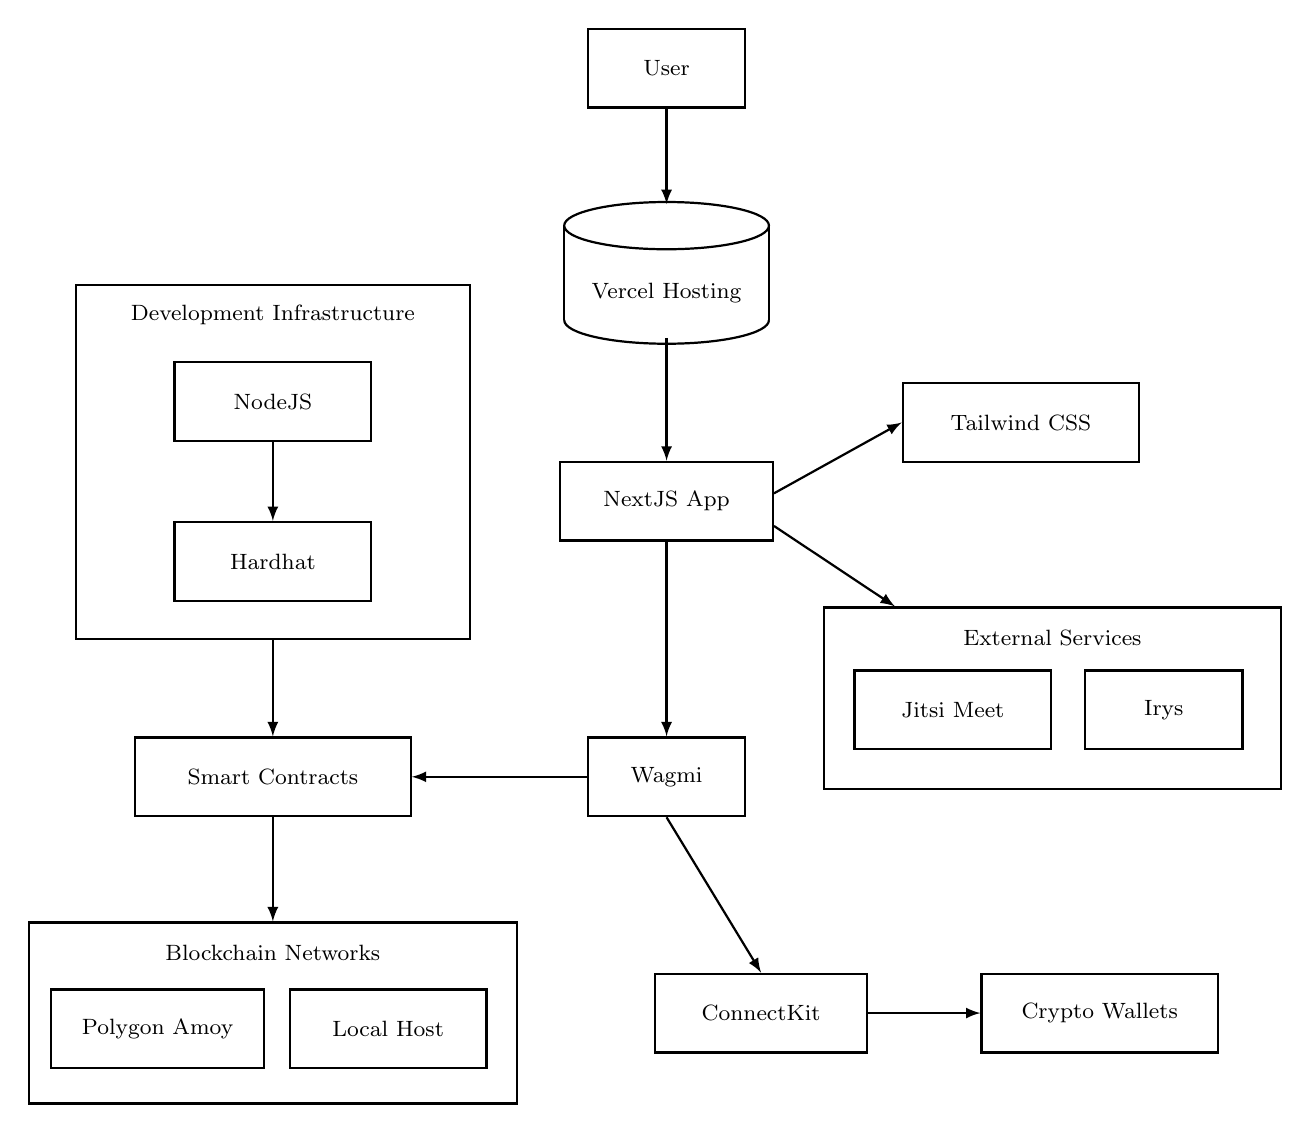
\begin{tikzpicture}
    \tikzset{
      pics/cylinder/.style={
          code={
              \draw[thick] (0,0) ellipse (1.3 and 0.3);

              \draw[thick] (-1.3,0) -- (-1.3,-1.2);
              \draw[thick] (1.3,0) -- (1.3,-1.2);

              \draw[thick] (-1.3,-1.2) arc (180:360:1.3 and 0.3);

              \node at (0,-0.85) {\footnotesize Vercel Hosting};
            }
        }
    }
    \node[draw, thick, rectangle, minimum width=2cm, minimum height=1cm, font=\footnotesize] (user) at (0, 0) {User};
    \pic (vercel) at (0, -2) {cylinder};
    \node (vercel_north) at (0, -1.85) {};
    \node (vercel_south) at (0, -3.3) {};

    \node[draw, thick, rectangle, minimum width=2.7cm, minimum height=1cm, font=\footnotesize] (nextjs) at (0, -5.5) {NextJS App};
    \node[draw, thick, rectangle, minimum width=3cm, minimum height=1cm, font=\footnotesize] (tailwindcss) at (4.5, -4.5) {Tailwind CSS};

    \node[draw, thick, rectangle, minimum width=5.8cm, minimum height=2.3cm, font=\footnotesize] (externalservice) at (4.9, -8) {};
    \node[font=\footnotesize] at ([yshift=-0.4cm]externalservice.north) {External Services};
    \node[draw, thick, rectangle, minimum width=2.5cm, minimum height=1cm, font=\footnotesize] (jitsimeet) at ([xshift=1.65cm, yshift=-0.15cm]externalservice.west) {Jitsi Meet};
    \node[draw, thick, rectangle, minimum width=2cm, minimum height=1cm, font=\footnotesize] (irys) at ([xshift=-1.5cm, yshift=-0.15cm]externalservice.east) {Irys};

    \node[draw, thick, rectangle, minimum width=5cm, minimum height=4.5cm, font=\footnotesize] (devinfrastructure) at (-5, -5) {};
    \node[font=\footnotesize] at ([yshift=-0.4cm]devinfrastructure.north) {Development Infrastructure};
    \node[draw, thick, rectangle, minimum width=2.5cm, minimum height=1cm, font=\footnotesize] (nodejs) at ([yshift=-1.5cm]devinfrastructure.north) {NodeJS};
    \node[draw, thick, rectangle, minimum width=2.5cm, minimum height=1cm, font=\footnotesize] (hardhat) at ([yshift=1cm]devinfrastructure.south) {Hardhat};

    \node[draw, thick, rectangle, minimum width=6.2cm, minimum height=2.3cm, font=\footnotesize] (network) at (-5, -12) {};
    \node[font=\footnotesize] at ([yshift=-0.4cm]network.north) {Blockchain Networks};
    \node[draw, thick, rectangle, minimum width=2.7cm, minimum height=1cm, font=\footnotesize] (amoytestnet) at ([xshift=1.65cm, yshift=-0.2cm]network.west) {Polygon Amoy};
    \node[draw, thick, rectangle, minimum width=2.5cm, minimum height=1cm, font=\footnotesize] (localhost) at ([xshift=-1.65cm, yshift=-0.2cm]network.east) {Local Host};

    \node[draw, thick, rectangle, minimum width=3.5cm, minimum height=1cm, font=\footnotesize] (smartcontracts) at (-5, -9) {Smart Contracts};
    \node[draw, thick, rectangle, minimum width=2cm, minimum height=1cm, font=\footnotesize] (wagmi) at (0, -9) {Wagmi};
    \node[draw, thick, rectangle, minimum width=2.7cm, minimum height=1cm, font=\footnotesize] (connectkit) at (1.2, -12) {ConnectKit};
    \node[draw, thick, rectangle, minimum width=3cm, minimum height=1cm, font=\footnotesize] (cryptowallet) at (5.5, -12) {Crypto Wallets};

    \draw[-latex, thick] (user.south) -- (vercel_north);
    \draw[-latex, thick] (vercel_south) -- (nextjs.north);
    \draw[-latex, thick] ([yshift=0.1cm]nextjs.east) -- (tailwindcss.west);
    \draw[-latex, thick] ([yshift=0.2cm]nextjs.south east) -- ([xshift=-2cm]externalservice.north);
    \draw[-latex, thick] (nextjs.south) -- (wagmi.north);
    \draw[-latex, thick] (wagmi.south) -- (connectkit.north);
    \draw[-latex, thick] (connectkit.east) -- (cryptowallet.west);
    \draw[-latex, thick] (nodejs.south) -- (hardhat.north);
    \draw[-latex, thick] (wagmi.west) -- (smartcontracts.east);
    \draw[-latex, thick] (devinfrastructure.south) -- (smartcontracts.north);
    \draw[-latex, thick] (smartcontracts.south) -- (network.north);
  \end{tikzpicture}
  \caption{Sơ đồ kiến trúc hệ thống}
  \label{fig:system-architecture}
\end{figure}

\subsection{Thành phần giao diện người dùng}

Giao diện người dùng được phát triển bằng framework \textbf{NextJS} và triển khai trên nền tảng \textbf{Vercel}, hỗ trợ hiệu năng cao và dễ dàng mở rộng.
Giao diện sử dụng \textbf{Tailwind CSS} để xây dựng UI hiện đại, tối ưu cho trải nghiệm người dùng. Toàn bộ tương tác của người dùng với hệ thống (tham gia thử thách, gửi giải pháp, truy xuất hồ sơ uy tín...) đều diễn ra thông qua lớp này.

\subsection{Tương tác với blockchain}

Để frontend tương tác với blockchain, hệ thống sử dụng thư viện \textbf{Wagmi} kết hợp với \textbf{ConnectKit} giúp tích hợp ví tiền điện tử như MetaMask hoặc CoinBase.
Các chức năng như xác thực người dùng qua ví, gửi giao dịch on-chain, theo dõi sự kiện blockchain đều được xử lý tại đây.

\subsection{Hợp đồng thông minh và hạ tầng blockchain}

Các hợp đồng thông minh được phát triển bằng \textbf{Solidity}, biên dịch và triển khai thông qua \textbf{Hardhat}. Trong quá trình phát triển và thử nghiệm, hệ thống hỗ trợ triển khai trên mạng cục bộ và mạng thử nghiệm \textbf{Polygon Amoy}.
Các chức năng chính của smart contract bao gồm: quản lý thử thách, giải pháp và thông tin tuyển dụng, quản lý thông tin cá nhân và hồ sơ uy tín của người dùng và nhà tuyển dụng, kiểm soát truy cập.

\subsection{Các dịch vụ bên ngoài}

Một số loại dữ liệu không phù hợp để lưu trực tiếp trên chuỗi như nội dung thử thách hoặc giải pháp sẽ được lưu trữ trên \textbf{Irys}, với CID được lưu lại trên blockchain để dễ dàng tham chiếu.
Ngoài ra, hệ thống còn tích hợp \textbf{Jitsi Meet} để phục vụ việc tổ chức các buổi phỏng vấn trực tuyến giữa nhà tuyển dụng và ứng viên, đảm bảo tính riêng tư và tiện lợi.

% // TODO: Ghi nội dung sau khi có sơ đồ
\section{Mô hình dữ liệu}

\section{Chi tiết các hợp đồng thông minh}

\subsection{Danh sách các hợp đồng chính}

Hệ thống SkillChain được tổ chức thành nhiều hợp đồng thông minh độc lập theo nguyên tắc phân tách trách nhiệm. Mỗi hợp đồng đảm nhiệm một vai trò riêng trong hệ thống và được triển khai độc lập để tăng khả năng bảo trì, tái sử dụng và kiểm soát truy cập. Dưới đây là danh sách các hợp đồng chính trong hệ thống:

\begin{itemize}
  \item \textbf{UserDataManager}: Quản lý thông tin cá nhân và định danh người dùng.
  \item \textbf{ReputationManager}: Lưu trữ và cập nhật hồ sơ uy tín của người dùng, bao gồm điểm uy tín toàn cục và điểm uy tín chuyên môn theo từng lĩnh vực. Hợp đồng này là trung tâm của hệ thống uy tín.
  \item \textbf{ChallengeManager}: Quản lý vòng đời của thử thách, từ khởi tạo, kiểm duyệt đến cho phép người dùng tham gia.
  \item \textbf{ModerationEscrow}: Điều phối việc phân phối phần thưởng token cho những người kiểm duyệt thử thách sau khi quá trình kiểm duyệt hoàn tất.
  \item \textbf{ChallengeCostManager}: Tính toán mức phí mà người dùng cần chi trả để tham gia vào một thử thách cụ thể.
  \item \textbf{SolutionManager}: Quản lý quá trình người dùng thực hiện và gửi giải pháp cho thử thách, ghi nhận hành vi nộp bài, và xử lý luồng đánh giá bởi các người đánh giá.
  \item \textbf{RecruiterDataManager}: Quản lý thông tin tài khoản nhà tuyển dụng.
  \item \textbf{RecruiterSubscription}: Kiểm soát việc thanh toán phí đăng ký theo chu kỳ từ phía nhà tuyển dụng để có quyền đăng bài tuyển dụng trên hệ thống.
  \item \textbf{JobManager}: Lưu trữ và quản lý các bài đăng tuyển dụng.
  \item \textbf{JobApplicationManager}: Ghi nhận và quản lý thông tin ứng tuyển của người dùng cho từng bài đăng cụ thể.
  \item \textbf{MeetingManager}: Tổ chức và lưu trữ lịch họp trực tuyến giữa nhà tuyển dụng và ứng viên.
  \item \textbf{RoleManager}: Phân quyền hệ thống, kiểm soát ai được phép gọi các chức năng đặc biệt. Hợp đồng này đảm bảo an toàn và tách biệt vai trò trong hệ thống.
\end{itemize}

\subsection{ReputationManager}

Hợp đồng \textbf{ReputationManager} chịu trách nhiệm duy trì, cập nhật và điều chỉnh các chỉ số uy tín của người dùng theo từng lĩnh vực chuyên môn cũng như tổng điểm uy tín toàn cục.
Đây là thành phần cốt lõi để xác định vai trò, quyền truy cập và độ tin cậy của người tham gia trên nền tảng SkillChain.

\subsubsection{Chức năng chính}

\begin{itemize}
  \item Ghi nhận và duy trì điểm uy tín theo từng lĩnh vực chuyên môn và tổng uy tín toàn cục.
  \item Tính toán và cập nhật sự thay đổi uy tín dựa trên hành vi của người dùng trong các vai trò người giải thử thách, người đóng góp, người kiểm duyệt và người đánh giá giải pháp. Cơ chế cập nhật đã được giải thích chi tiết tại mục 3.2.
  \item Tự động cấp hoặc thu hồi vai trò tùy theo mức uy tín đạt được.
\end{itemize}

\subsubsection{Các hàm chức năng chính}

\begin{itemize}
  \item \texttt{updateSolvingProblemReputation}: cập nhật uy tín người giải thử thách sau khi giải pháp đã được đánh giá
  \item \texttt{updateEvaluateSolutionReputation}: cập nhật uy tín người đánh giá giải pháp sau khi phiên đánh giá kết thúc
  \item \texttt{updateContributionReputation}: cập nhật uy tín người đóng góp sau khi thử thách đã được duyệt xong
  \item \texttt{updateModerationReputation}: cập nhật uy tín người kiểm duyệt sau khi phiên kiểm duyệt hoàn tất
\end{itemize}

\subsubsection{Tương tác với hợp đồng khác}

\begin{itemize}
  \item \textbf{RoleManager}: Cấp hoặc thu hồi vai trò sau khi uy tín thay đổi
  \item \textbf{ChallengeManager}: Cập nhật uy tín sau khi phiên kiểm duyệt thử thách hoàn tất
  \item \textbf{SolutionManager}: Cập nhật uy tín sau khi phiên đánh giá giải pháp kết thúc
\end{itemize}

% // TODO: Giải thích về RoleManager nếu cần thiết

\subsection{ChallengeManager}

Hợp đồng \textbf{ChallengeManager} đóng vai trò trung tâm trong quá trình quản lý các thử thách kỹ năng trong hệ thống SkillChain.
Hợp đồng này chịu trách nhiệm cho toàn bộ vòng đời của một thử thách -- từ khởi tạo, đóng góp, kiểm duyệt cho đến tham gia thử thách và cập nhật dữ liệu uy tín.

\subsubsection{Chức năng chính}

\begin{itemize}
  \item Cho phép người đóng góp tạo và gửi thử thách cho bên kiểm duyệt
  \item Cho phép người kiểm duyệt tham gia kiểm duyệt và đánh giá chất lượng thử thách
  \item Hợp nhất kết quả kiểm duyệt theo mô hình có trọng số dựa trên uy tín, từ đó phân phối token cho bên kiểm duyệt và cập nhật uy tín cho người đóng góp và từng người kiểm duyệt
  \item Cho phép người dùng tham gia thử thách, hỗ trợ tính toán lượng token cần phải trả cho người đóng góp để tham gia
\end{itemize}

\subsubsection{Cấu trúc dữ liệu chính}

\begin{itemize}
  \item \texttt{Challenge}: chứa thông tin đầy đủ của một thử thách
  \item \texttt{ModeratorReview}: ghi nhận đánh giá của từng người kiểm duyệt đối với một thử thách
  \item \texttt{ReviewPool}: tập hợp những người kiểm duyệt tham gia vào một thử thách và trạng thái kiểm duyệt
  \item \texttt{JoinedChallenges}: ghi nhận thử thách mà người dùng đã và đang tham gia giải
\end{itemize}

\subsubsection{Các hàm chức năng chính}

\paragraph{Quản lý thử thách}

\begin{itemize}
  \item \texttt{createChallenge}: Người dùng có đủ quyền đóng góp trong một lĩnh vực chuyên môn có thể khởi tạo thử thách nháp
  \item \texttt{contributeChallenge}: Người đóng góp chính thức gửi thử thách cho bên kiểm duyệt, đính kèm mức token treo thưởng.
\end{itemize}

\paragraph{Kiểm duyệt thử thách}

\begin{itemize}
  \item \texttt{joinReviewPool}: Cho phép người kiểm duyệt hợp lệ tham gia vào phiên kiểm duyệt
  \item \texttt{submitModeratorReview}: Gửi đánh giá chất lượng thử thách, tính điểm theo các yếu tố chất lượng
  \item \texttt{finalizeChallenge}: Khi đủ số lượng đánh giá, hợp nhất kết quả yếu tố chất lượng, xác định mức độ khó, tính thời gian giải ước tính, tính điểm chất lượng, cập nhật uy tín và phân phối token.
\end{itemize}

\paragraph{Người dùng tham gia thử thách}

\begin{itemize}
  \item \texttt{userJoinChallenge}: Người dùng trả phí token, tham gia thử thách và khởi tạo không gian giải pháp
  \item \texttt{userCompleteChallenge}: Cập nhật số người hoàn thành
\end{itemize}

% // TODO: Giải thích cách tổng hợp kết quả kiểm duyệt
\subsubsection{Cơ chế hợp nhất kết quả kiểm duyệt}

Giả sử $D$ là tập hợp mức độ khó của thử thách (dễ, trung bình, khó), $M$ là tập hợp các người kiểm duyệt đánh giá một thử thách. Với mỗi người kiểm duyệt $m \in M$, ta có:
\begin{itemize}
  \item $d_m$ là độ khó đã đề xuất
  \item $t_m$ là thời gian giải ước tính đã đề xuất
  \item $w_m$ là điểm uy tín chuyên môn trong lĩnh vực tương ứng của thử thách
\end{itemize}

\paragraph{Xác định mức độ khó}

\paragraph{Tính thời gian giải ước tính}

\paragraph{Tính điểm chất lượng}

\subsubsection{Tương tác với hợp đồng khác}

\begin{itemize}
  \item \textbf{ReputationManager}: Cập nhật uy tín sau khi phiên kiểm duyệt chất lượng thử thách kết thúc
  \item \textbf{RoleManager}: Kiểm soát quyền gọi hàm dựa trên chỉ số uy tín của người gọi
  \item \textbf{SolutionManager}: Phối hợp để quản lý thử thách mà người dùng tham gia
  \item \textbf{ChallengeCostManager}: Tính toán khoản token để tham gia thử thách
\end{itemize}

\subsection{ModeratorEscrow}

Hợp đồng \textbf{ModerationEscrow} đóng vai trò như một ``kho quỹ ký gửi'' để tạm giữ khoản token thưởng do người đóng góp nạp vào khi tạo thử thách.
Sau khi thử thách được kiểm duyệt và hợp nhất kết quả, hợp đồng này sẽ tính toán và phân phối phần thưởng cho các người kiểm duyệt phù hợp, dựa trên mức độ chính xác của kết quả kiểm duyệt và uy tín chuyên môn.

\subsubsection{Chức năng chính}

\begin{itemize}
  \item Nhận và lưu trữ token bounty từ người đóng góp
  \item Ghi nhận danh sách người kiểm duyệt tham gia
  \item Đánh giá độ lệch giữa điểm số của từng người kiểm duyệt với điểm số trung bình cuối cùng
  \item Tính trọng số và phân phối phần thưởng công bằng dựa trên uy tín và mức độ chính xác
\end{itemize}

\subsubsection{Các hàm chức năng chính}

\paragraph{Giao tiếp với người đóng góp}

\begin{itemize}
  \item \texttt{depositBounty}: Được gọi bởi \textbf{ChallengeManager} để lưu mức treo thưởng do người đóng góp cung cấp khi gửi thử thách.
\end{itemize}

\paragraph{Giao tiếp với người kiểm duyệt}

\begin{itemize}
  \item \texttt{syncModeratorsFromReviewPool}: Đồng bộ danh sách kiểm duyệt từ \textbf{ChallengeManager} vào \textbf{ModerationEscrow}
  \item \texttt{finalizeChallengePot}: Thực hiện phân phối token sau khi thử thách được duyệt xong
\end{itemize}

% // TODO: Giải thích cách phân phối token
\subsubsection{Cơ chế phân phối token}

\subsubsection{Tương tác với hợp đồng khác}

\begin{itemize}
  \item \textbf{ReputationManager}: Truy xuất thông tin uy tín của kiểm duyệt viên
  \item \textbf{ChallengeManager}: Hỗ trợ phân phối thưởng khi phiên kiểm duyệt hoàn tất
\end{itemize}

\subsection{ChallengeCostManager}

Hợp đồng \textbf{ChallengeCostManager} đảm nhiệm việc tính toán, thu thập và chuyển giao token phí từ người tham gia thử thách đến người đóng góp thử thách.
Nó giúp đảm bảo sự khuyến khích kinh tế rõ ràng cho người tạo nội dung và điều chỉnh giá trị tham gia dựa trên độ khó và chất lượng.

\subsubsection{Chức năng chính}

\begin{itemize}
  \item Tính phí tham gia thử thách
  \item Xử lý thanh toán từ người tham gia đến contributor khi đăng ký tham gia thử thách
  \item Ghi nhận tổng doanh thu và thông tin thanh toán theo từng thử thách
\end{itemize}

\subsubsection{Các hàm chức năng chính}

\begin{itemize}
  \item \texttt{\_computeCost}: tính lượng token để tham gia thử thách
  \item \texttt{addTalentPayment}: gửi token từ người tham gia cho người đóng góp và ghi nhận người tham gia đối với thử thách này
\end{itemize}

% // TODO: Giải thích cách tính phí tham gia
\subsubsection{Công thức tính phí}

\subsubsection{Tương tác với hợp đồng khác}

\begin{itemize}
  \item \textbf{ChallengeManager}: Hỗ trợ tính phí tham gia thử thách
  \item \textbf{ModeratorEscrow}: Dùng để lấy mức treo thưởng, phục vụ cho tính phí động
\end{itemize}

\subsection{SolutionManager}

Hợp đồng \textbf{SolutionManager} chịu trách nhiệm ghi nhận toàn bộ quy trình người dùng tham gia thử thách, nộp giải pháp, đưa vào hệ thống đánh giá, cũng như tổng hợp kết quả đánh giá và cập nhật điểm uy tín.

\subsubsection{Chức năng chính}

\begin{itemize}
  \item Quản lý thông tin giải pháp của người dùng đối với mỗi thử thách
  \item Điều phối quá trình đánh giá giải pháp bằng cách tổ chức một phiên đánh giá gồm các người đánh giá
  \item Tính điểm trung bình có trọng số cho giải pháp, cập nhật tiến độ, lưu trữ điểm số và cập nhật điểm uy tín cho người giải và những người đánh giá
\end{itemize}

\subsubsection{Cấu trúc dữ liệu chính}

\begin{itemize}
  \item \texttt{Solution}: Chứa thông tin đầy đủ của một giải pháp
  \item \texttt{Evaluation}: Ghi nhận điểm số của người đánh giá đối với một giải pháp
  \item \texttt{EvaluationPool}: Tập hợp những người đánh giá tham gia vào một giải pháp và trạng thái đánh giá
\end{itemize}

\subsubsection{Các hàm chức năng chính}

\paragraph{Người dùng tham gia thử thách}

\begin{itemize}
  \item \texttt{createSolutionBase}: Ghi nhận hành vi tham gia thử thách và khởi tạo không gian giải pháp
\end{itemize}

\paragraph{Nộp và chuyển trạng thái giải pháp}

\begin{itemize}
  \item \texttt{submitSolution}: Người dùng nộp bài (không chỉnh sửa được nữa).
  \item \texttt{putSolutionUnderReview}: Chuyển giải pháp sang trạng thái chờ đánh giá và khởi tạo một phiên đánh giá.
\end{itemize}

\paragraph{Quản lý phiên đánh giá}

\begin{itemize}
  \item \texttt{evaluatorJoinSolution}: Cho phép người đánh giá tham gia đánh giá giải pháp
  \item \texttt{evaluatorSubmitScore}: Gửi điểm đánh giá
  \item \texttt{finalizeEvaluation}: Khi ghi nhận đủ điểm đánh giá, tính toán điểm giáp pháp cuối cùng và cập nhật uy tín cho người giải và những người đánh giá
\end{itemize}

% // TODO: Giải thích cách tính điểm đánh giá
\subsubsection{Cơ chế tổng hợp điểm đánh giá}

\subsubsection{Tương tác với hợp đồng khác}

\begin{itemize}
  \item \textbf{ReputationManager}: Cập nhật uy tín sau khi phiên đánh giá giải pháp kết thúc
  \item \textbf{ChallengeManager}: Phối hợp để quản lý thử thách mà người dùng đã tham gia
  \item \textbf{RoleManager}: Kiểm soát quyền gọi hàm
\end{itemize}

% // TODO: Giải thích về hợp đồng nếu cần thiết
\subsection{RecruiterSubscription}

\section{Giao diện xây dựng uy tín}

\subsection{Kết nối tài khoản}

Trước khi sử dụng hệ thống SkillChain, người dùng sẽ được yêu cầu kết nối với ví của mình.

\begin{figure}[H]
  \centering
  
\includegraphics[width=0.99\textwidth, frame]{ui/login.png}
  \caption{Trang kết nối tài khoản}
  \label{fig:login-page}
\end{figure}

Tại trang này, người dùng có thể nhấn nút ``Connect'' để chọn ví muốn kết nối.

\begin{figure}[H]
  \centering
  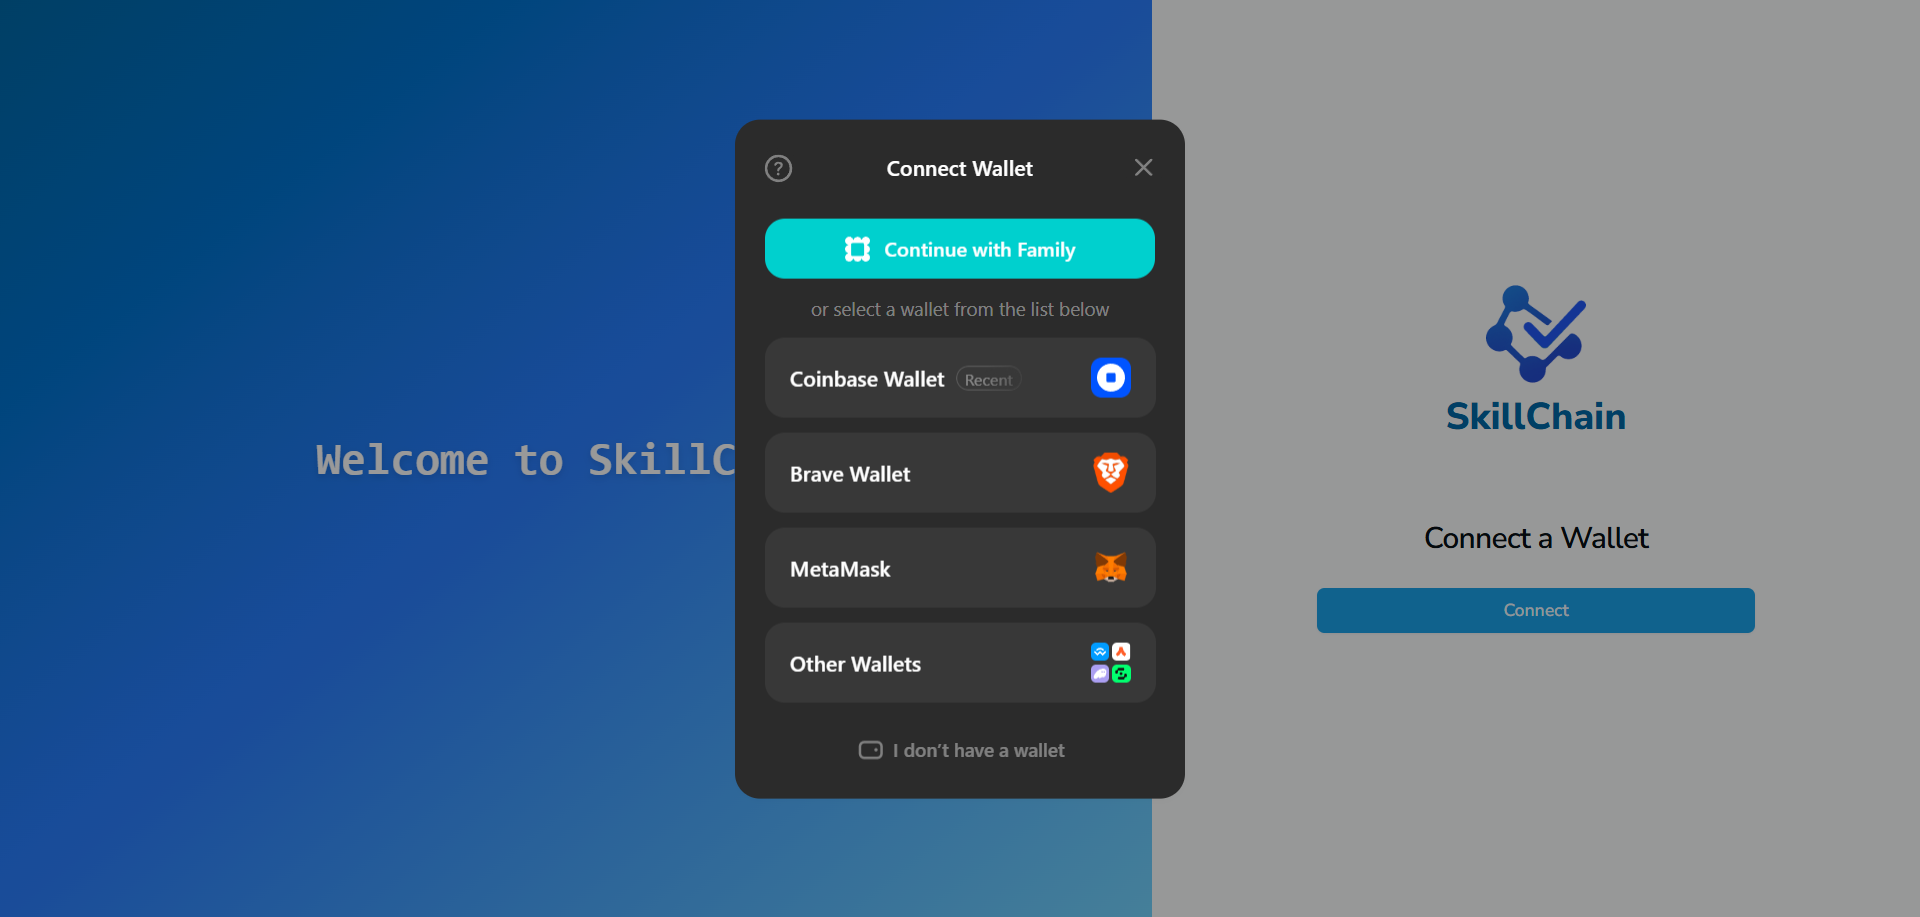
\includegraphics[width=0.99\textwidth, frame]{ui/login-wallets-page.png}
  \caption{Hộp thoại chọn ví kết nối}
  \label{fig:login-wallets-page}
\end{figure}

Sau khi kết nối thành công, hệ thống sẽ điều hướng người dùng đến trang chủ.

\begin{figure}[H]
  \centering
  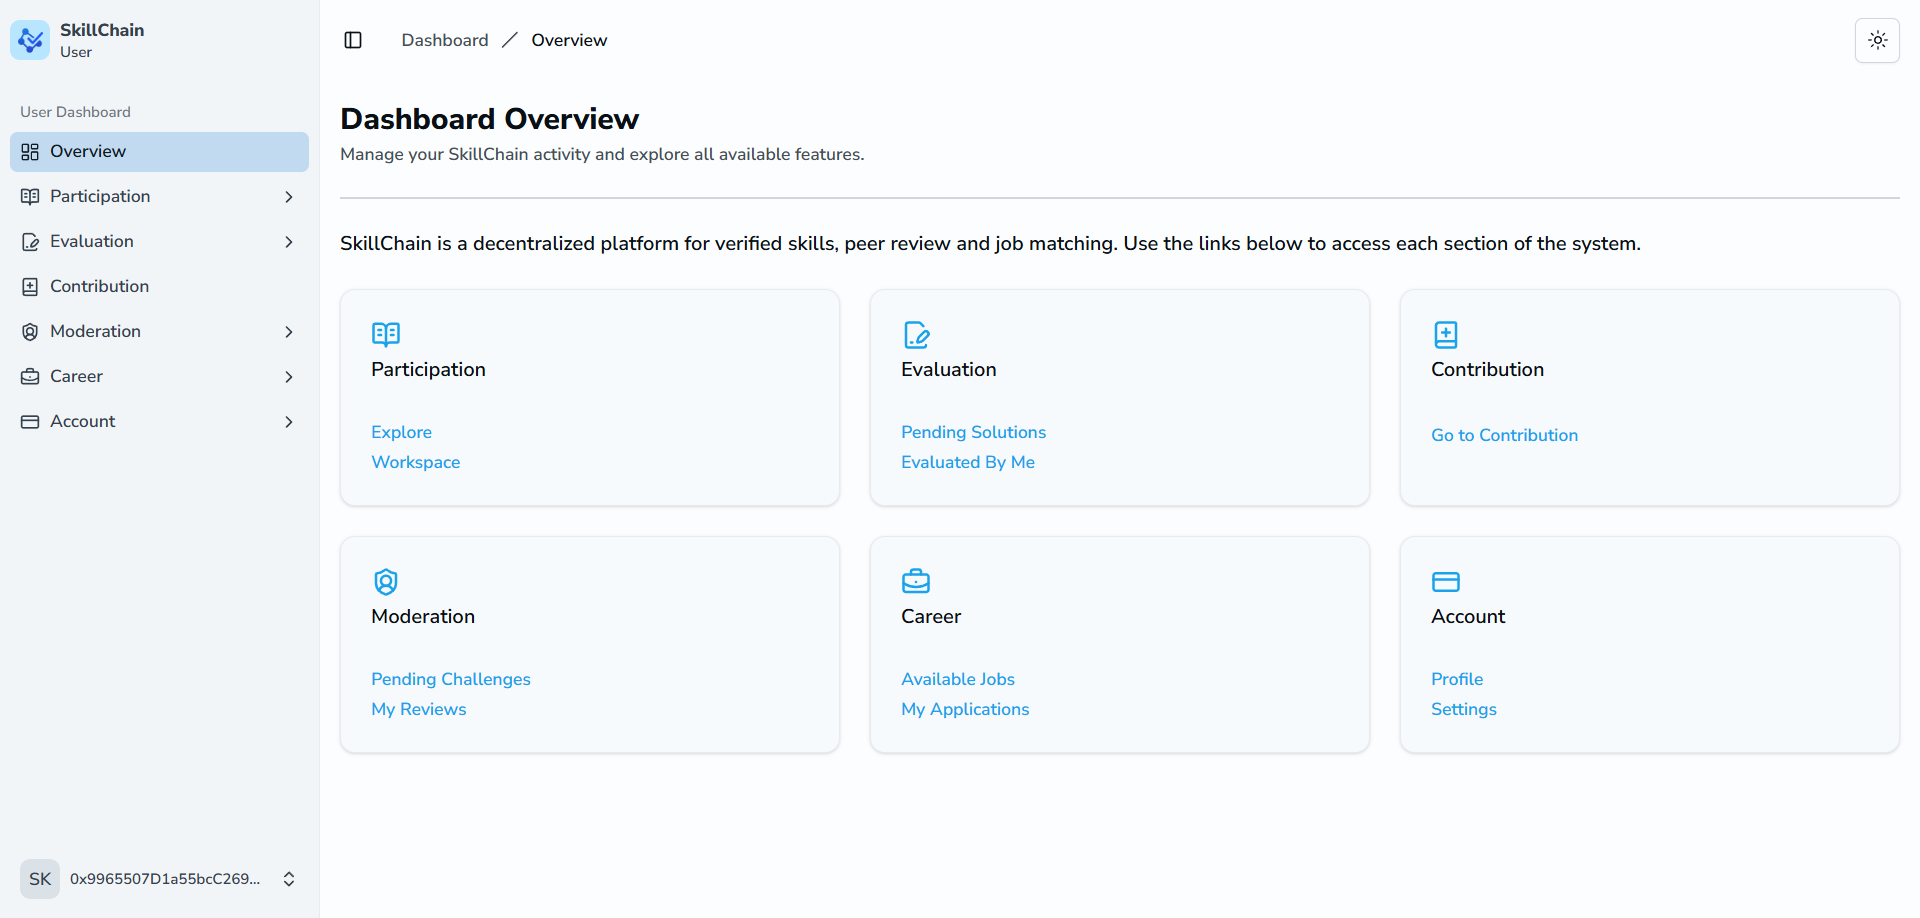
\includegraphics[width=0.99\textwidth, frame]{ui/home-page.png}
  \caption{Trang chủ}
  \label{fig:home-page}
\end{figure}

\subsection{Quản lý tài khoản}

\subsubsection{Thông tin cá nhân}

Để xem thông tin cá nhân, người dùng cần chọn \textbf{Account} $\rightarrow$ \textbf{Profile}.

\begin{figure}[H]
  \centering
  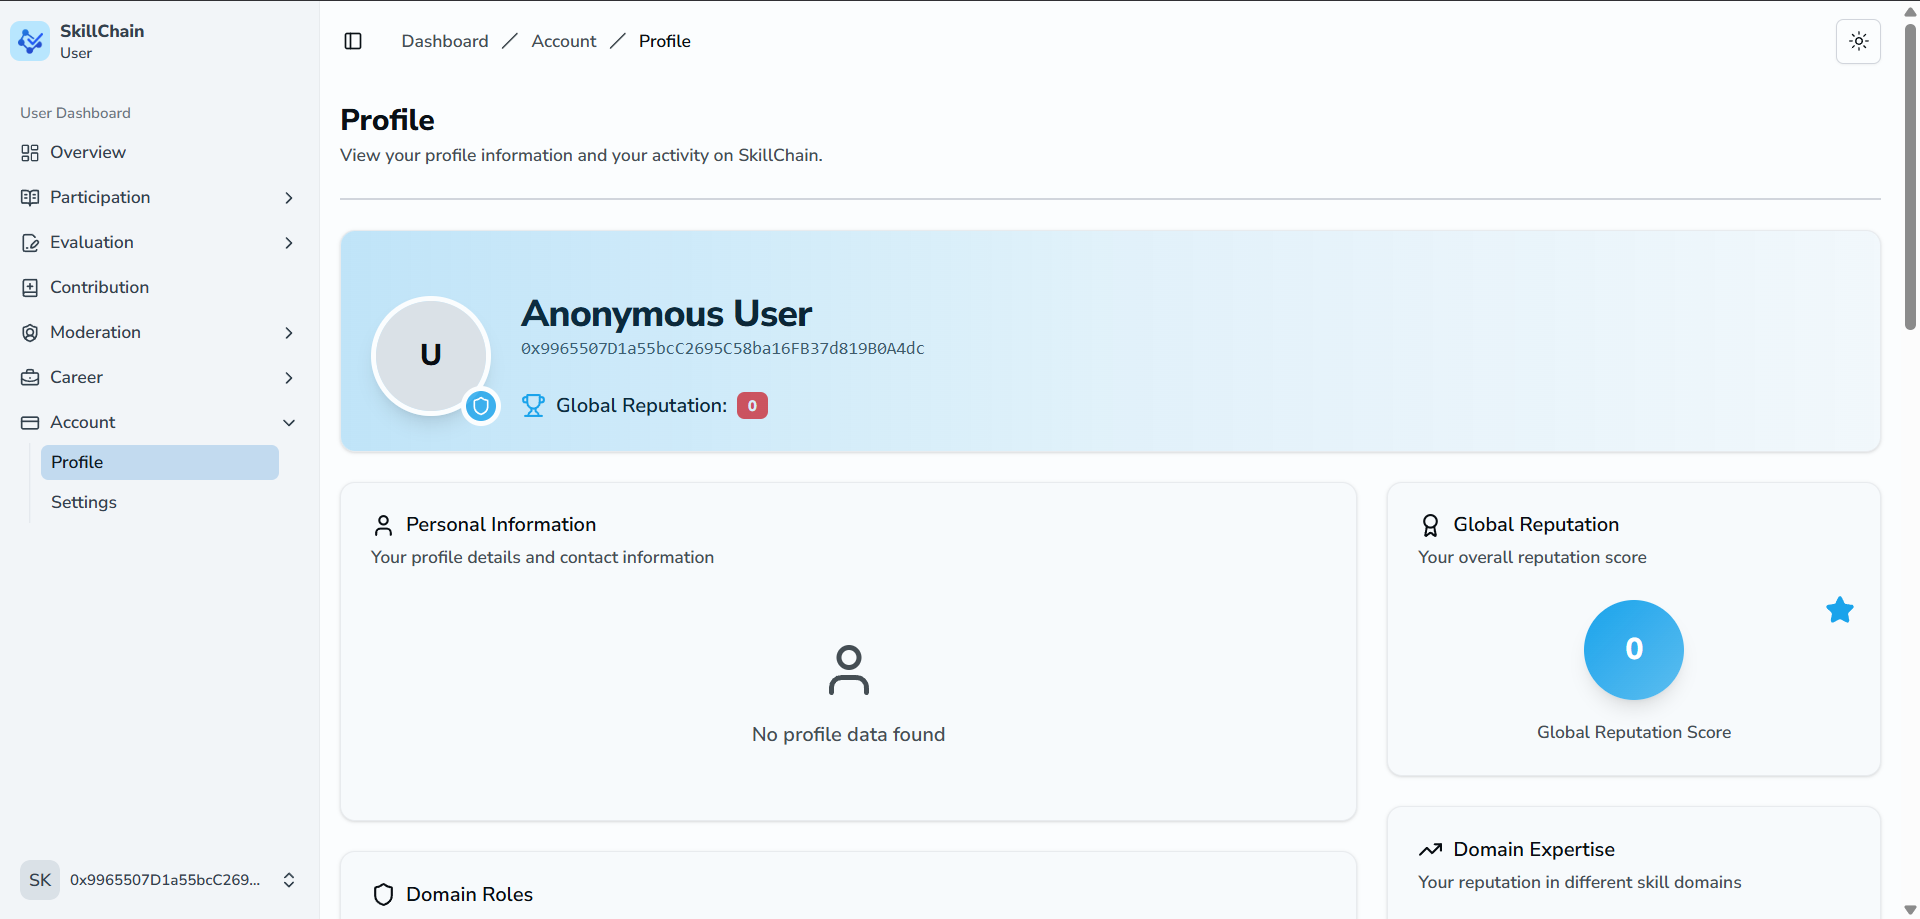
\includegraphics[width=0.99\textwidth, frame]{ui/unregistered-account-page.png}
  \caption{Trang thông tin tài khoản khi chưa đăng ký}
  \label{fig:unregistered-account-page}
\end{figure}

Ở góc dưới bên trái, hệ thống hiển thị quyền của người dùng đối với từng lĩnh vực chuyên môn, bao gồm khả năng đóng góp, kiểm duyệt và đánh giá.

\begin{figure}[H]
  \centering
  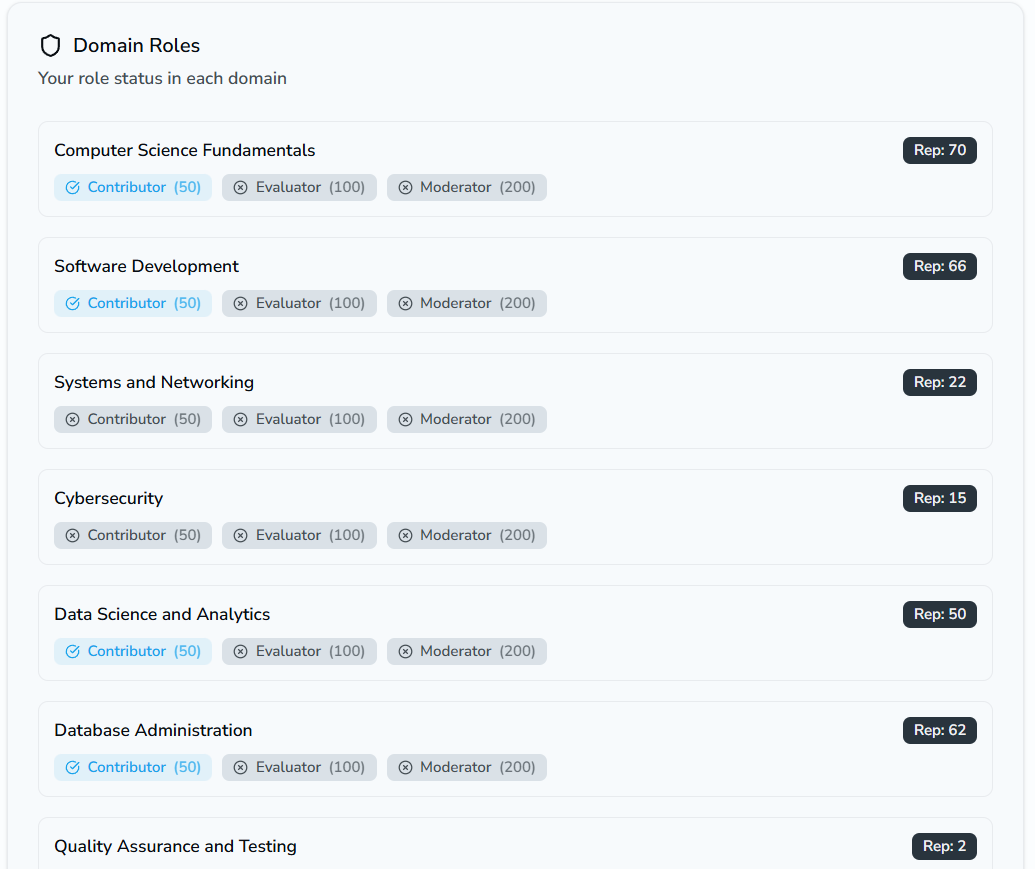
\includegraphics[width=0.99\textwidth, frame]{ui/domain-roles-page.png}
  \caption{Bảng vai trò của người dùng theo lĩnh vực chuyên môn}
  \label{fig:domain-roles-page}
\end{figure}

Hồ sơ uy tín được hiển thị ở góc dưới bên phải, bao gồm chỉ số uy tín toàn cục và uy tín theo từng lĩnh vực chuyên môn.

\begin{figure}[H]
  \centering
  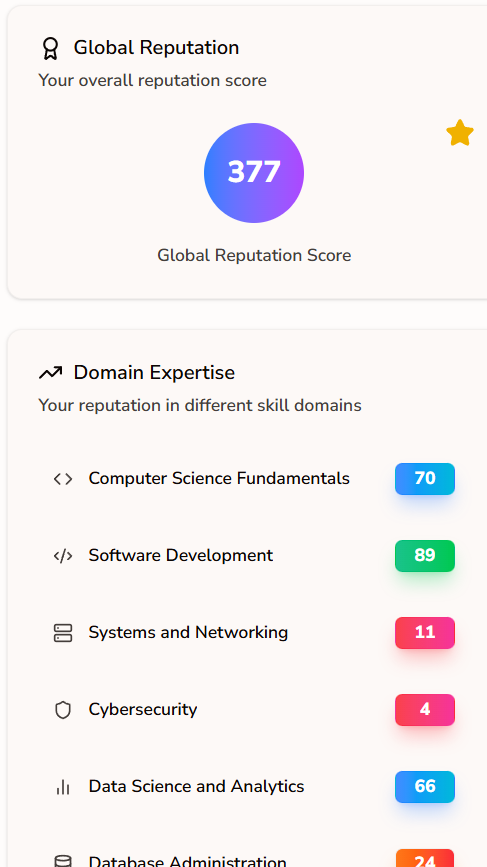
\includegraphics[width=0.5\textwidth, frame]{ui/reputation-profile.png}
  \caption{Hồ sơ uy tín}
  \label{fig:reputation-profile}
\end{figure}

\subsubsection{Cài đặt tài khoản}

Để chỉnh sửa thông tin cá nhân hoặc đăng ký tài khoản (nếu là lần kết nối đầu tiên), người dùng cần chọn \textbf{Account} $\rightarrow$ \textbf{Settings} và chuyển đến tab \textbf{Profile}.
Tại đây, người dùng có thể chọn ảnh đại diện, điền họ tên, địa chỉ email, nơi cư trú và tiểu sử để chỉnh sửa hoặc đăng ký thông tin cá nhân.  
Đối với lần đăng ký đầu tiên, hệ thống sẽ yêu cầu người dùng xác nhận giao dịch thông qua ví tiền điện tử để hoàn tất quá trình.

\begin{figure}[H]
  \centering
  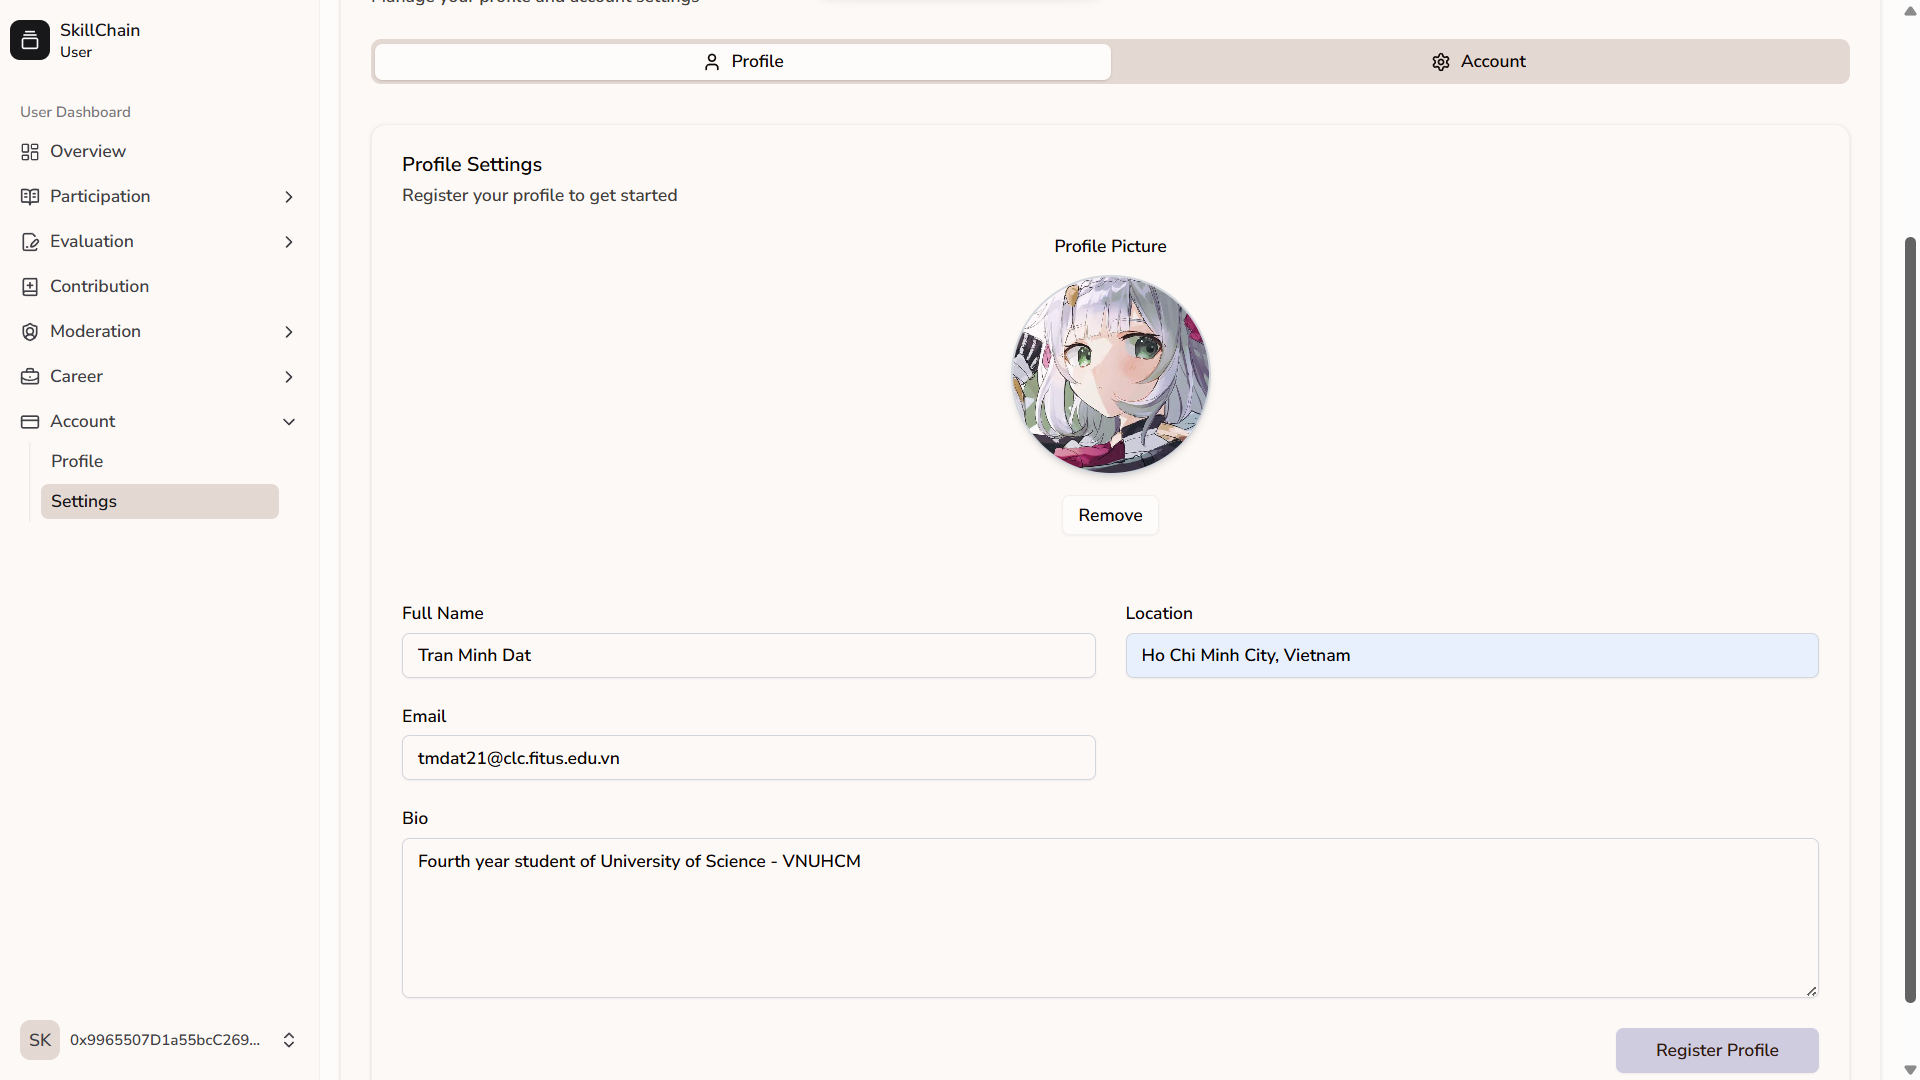
\includegraphics[width=0.99\textwidth, frame]{ui/register-account.png}
  \caption{Trang đăng ký thông tin cá nhân}
  \label{fig:register-account}
\end{figure}

\begin{figure}[H]
  \centering
  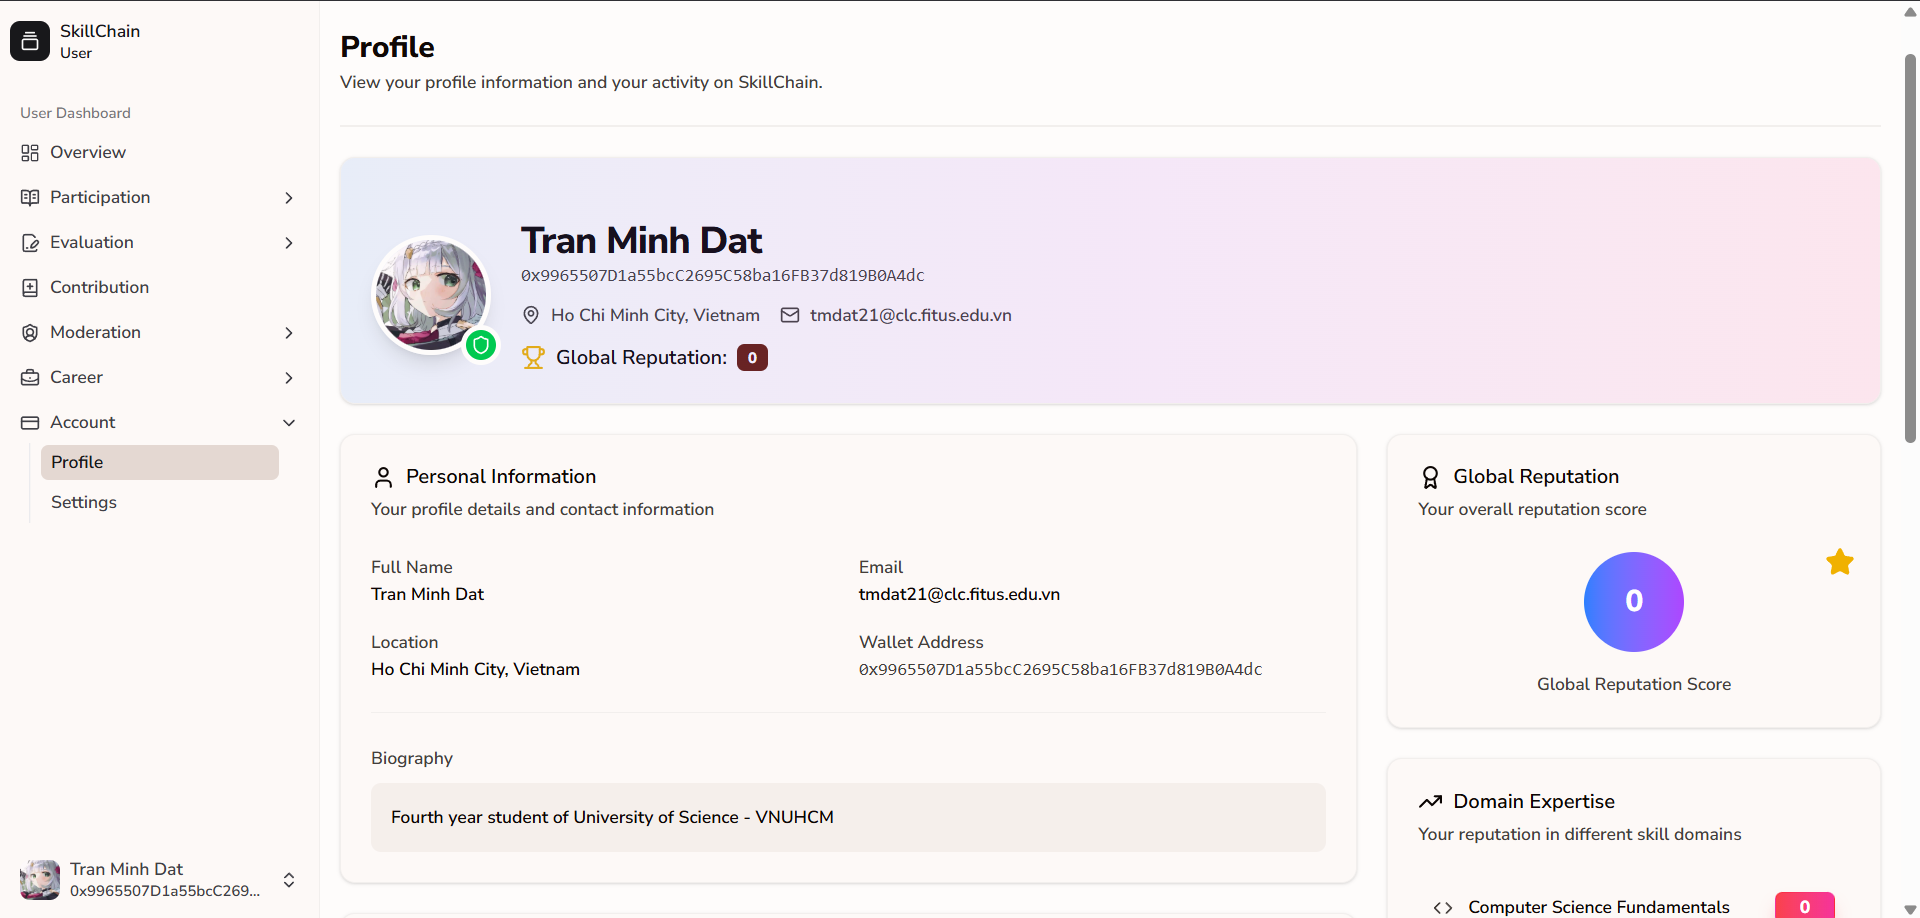
\includegraphics[width=0.99\textwidth, frame]{ui/registered-account-page.png}
  \caption{Trang thông tin cá nhân sau khi đã đăng ký}
  \label{fig:registered-account-page}
\end{figure}

Ngoài ra, người dùng cũng có thể truy cập tab \textbf{Account} để xem và cấu hình thông tin tài khoản liên quan đến hệ thống.

\begin{figure}[H]
  \centering
  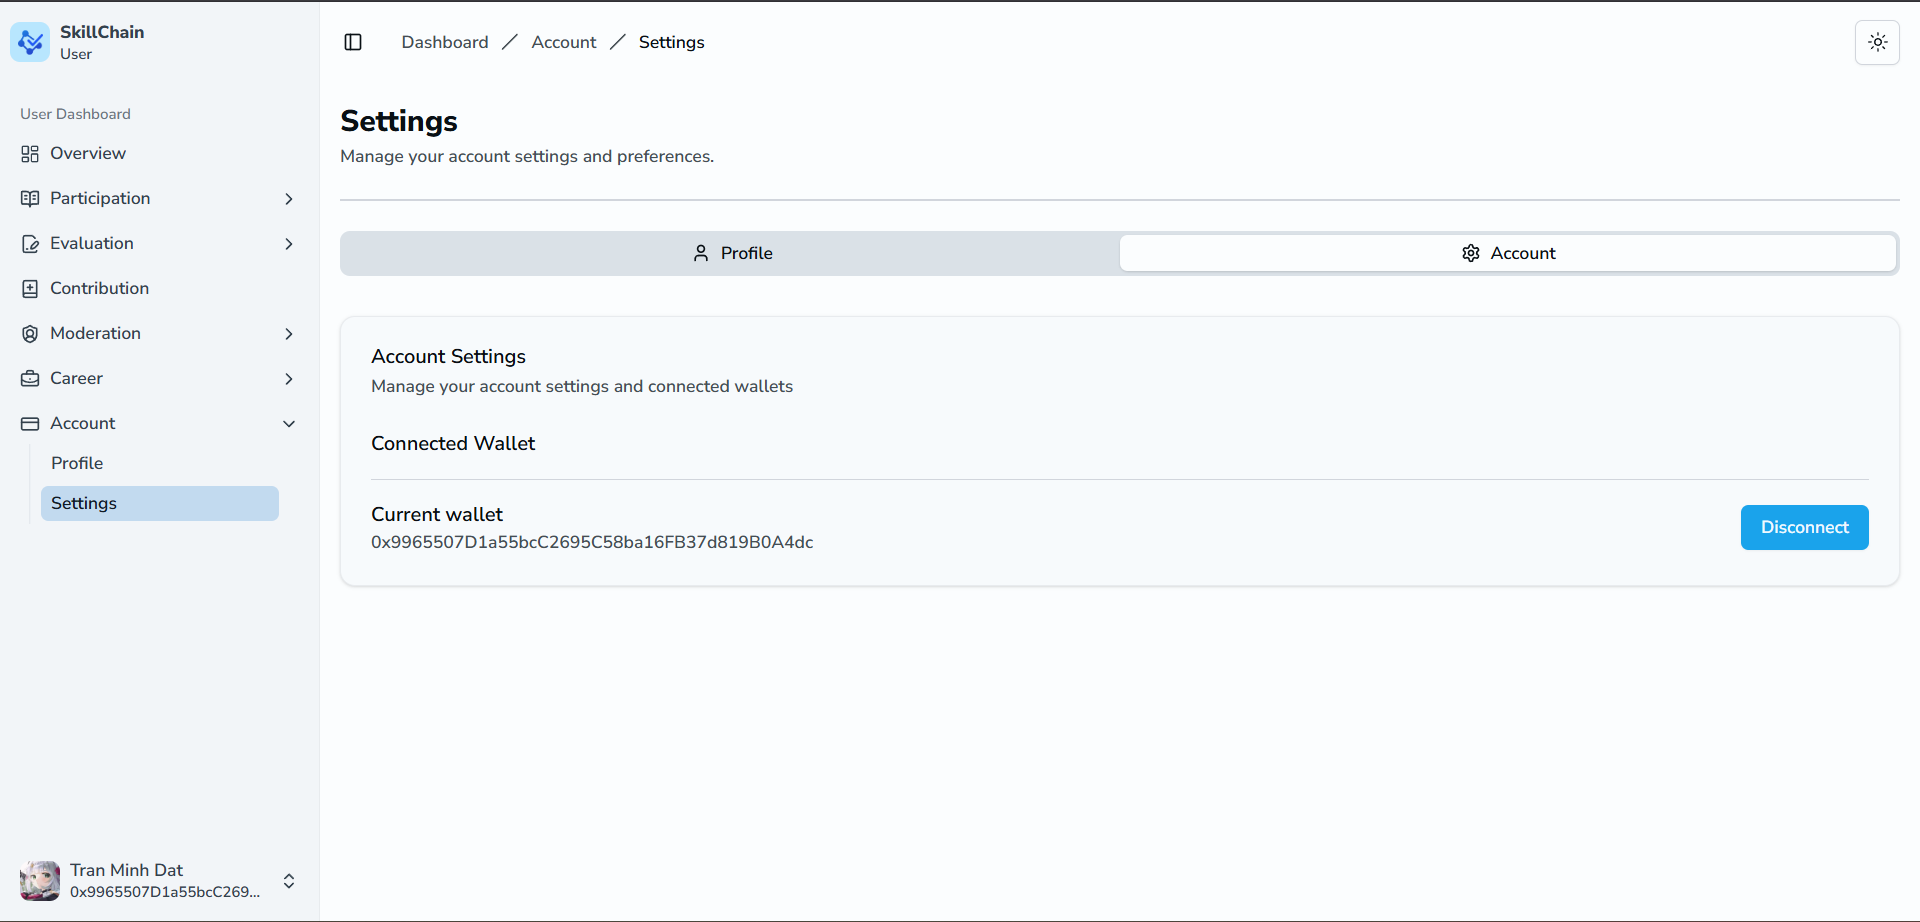
\includegraphics[width=0.99\textwidth, frame]{ui/account-settings-page.png}
  \caption{Trang thiết lập tài khoản}
  \label{fig:account-settings-page}
\end{figure}

\subsection{Đóng góp thử thách}

Để khởi tạo, quản lý và theo dõi các thử thách, người dùng cần truy cập tab \textbf{Contribution}.

\begin{figure}[H]
  \centering
  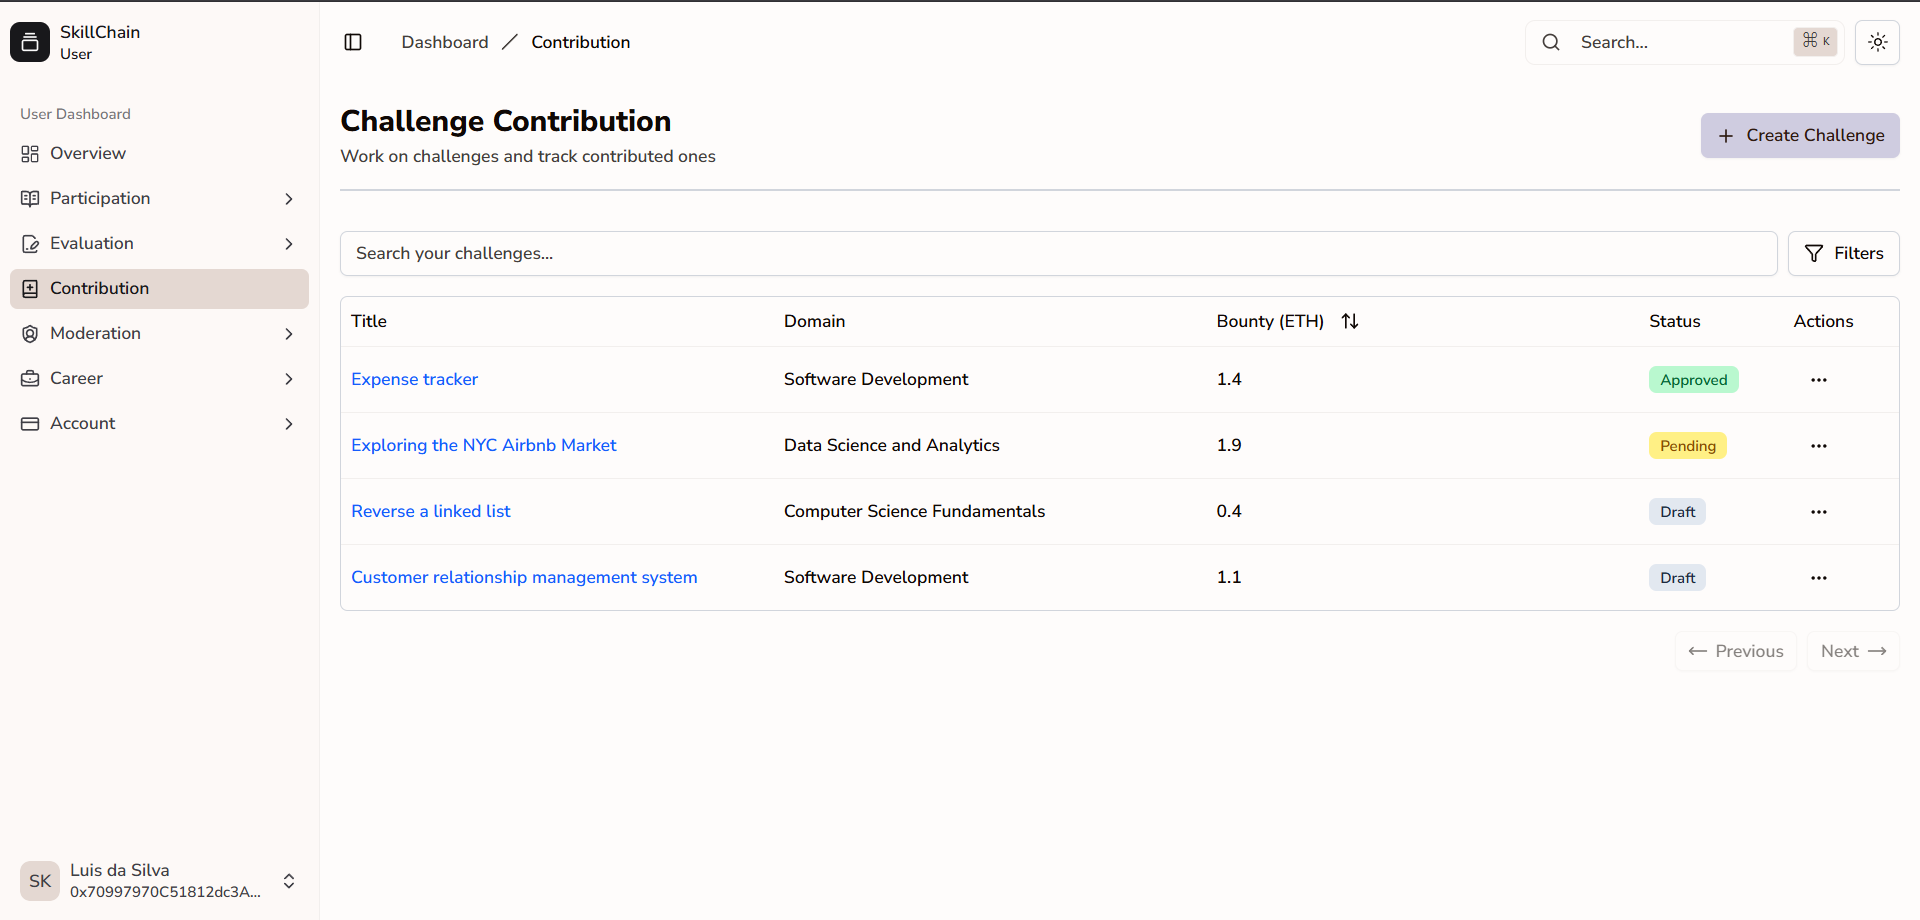
\includegraphics[width=0.99\textwidth, frame]{ui/contribution-page.png}
  \caption{Trang đóng góp thử thách}
  \label{fig:contribution-page}
\end{figure}

Tại đây, người dùng có thể xem danh sách các thử thách đã đóng góp, cùng với thông tin về loại thử thách, trạng thái và mức treo thưởng.  
Người dùng có thể xem chi tiết một thử thách bằng cách nhấn vào liên kết tên thử thách hoặc chọn ``View challenge'' từ nút ``Actions``.

\subsubsection{Tạo thử thách mới}

Để tạo một thử thách mới, người dùng nhấn nút ``Create Challenge'' ở góc trên bên phải.

\begin{figure}[H]
  \centering
  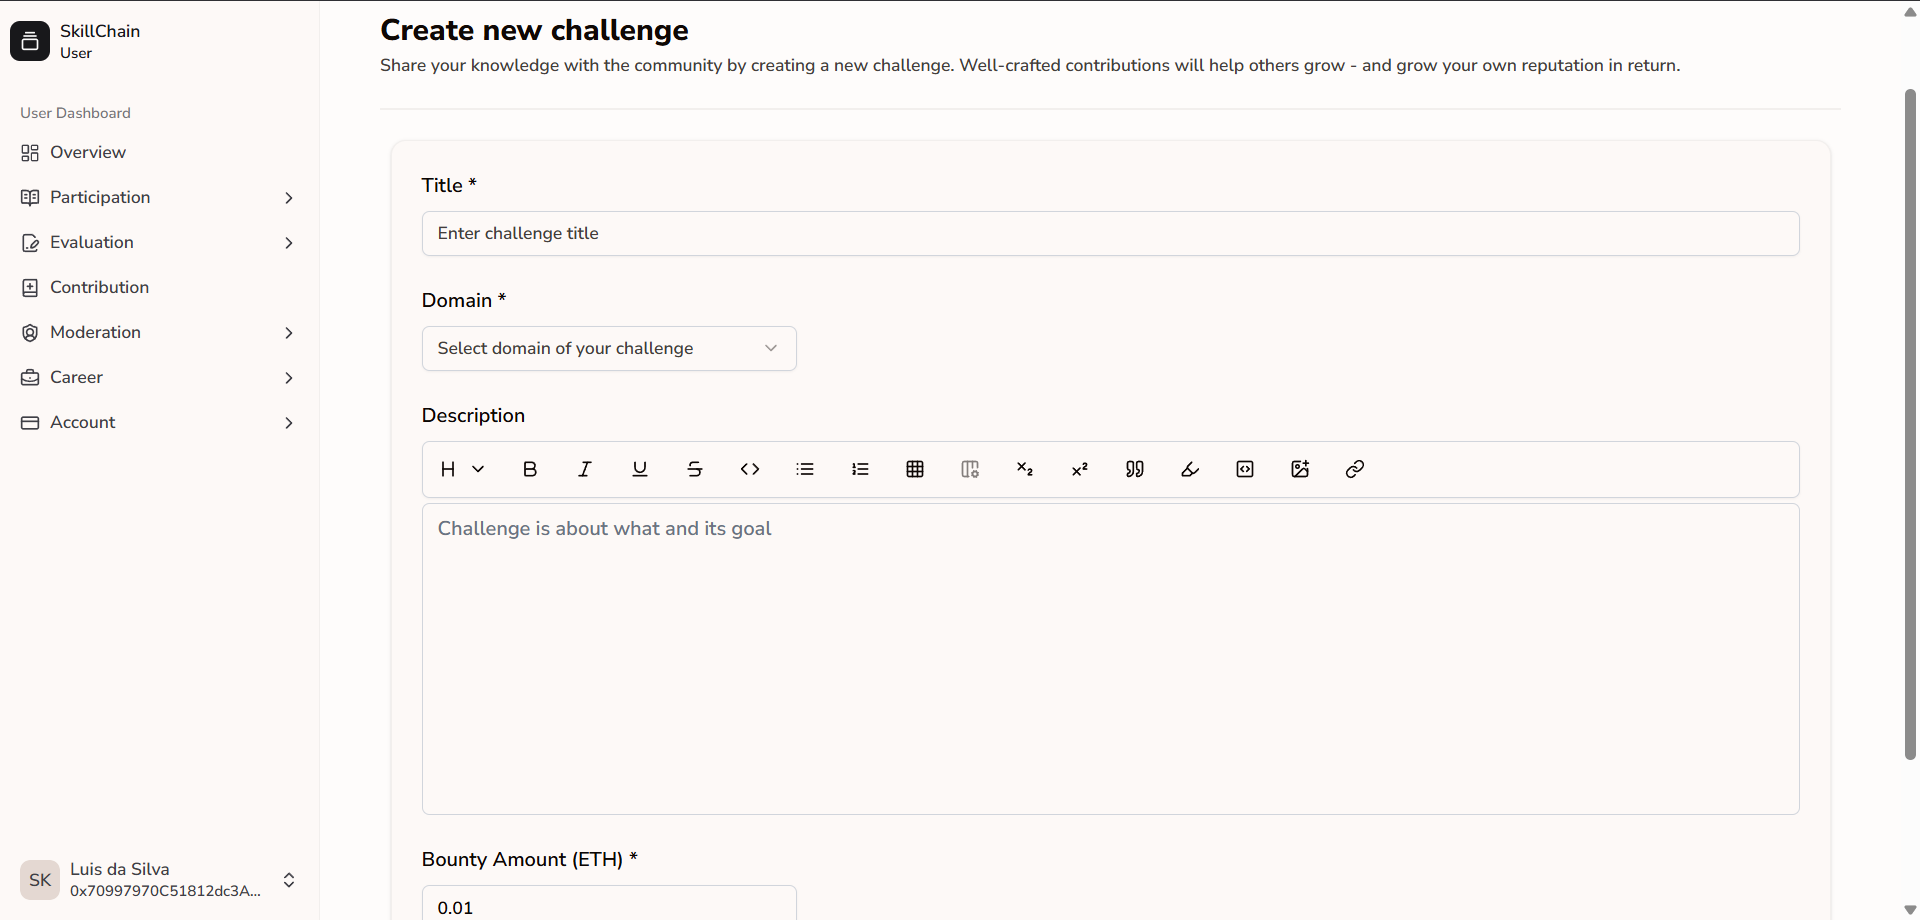
\includegraphics[width=0.99\textwidth, frame]{ui/create-challenge-page.png}
  \caption{Trang tạo thử thách mới}
  \label{fig:create-challenge-page}
\end{figure}

Tại trang này, người dùng nhập các thông tin quan trọng của thử thách, sau đó nhấn nút ``Create challenge''.  
Hệ thống sẽ yêu cầu xác thực giao dịch thông qua ví tiền điện tử để chính thức tạo thử thách ở trạng thái nháp.
Nếu người dùng không đủ chỉ số uy tín chuyên môn tương ứng với loại thử thách đang tạo, hệ thống sẽ hiển thị thông báo lỗi và không cho phép tạo thử thách.

\subsubsection{Chỉnh sửa thử thách}

Để chỉnh sửa một thử thách đang ở trạng thái nháp, người dùng cần truy cập trang chi tiết của thử thách và nhấn nút ``Edit''.

\begin{figure}[H]
  \centering
  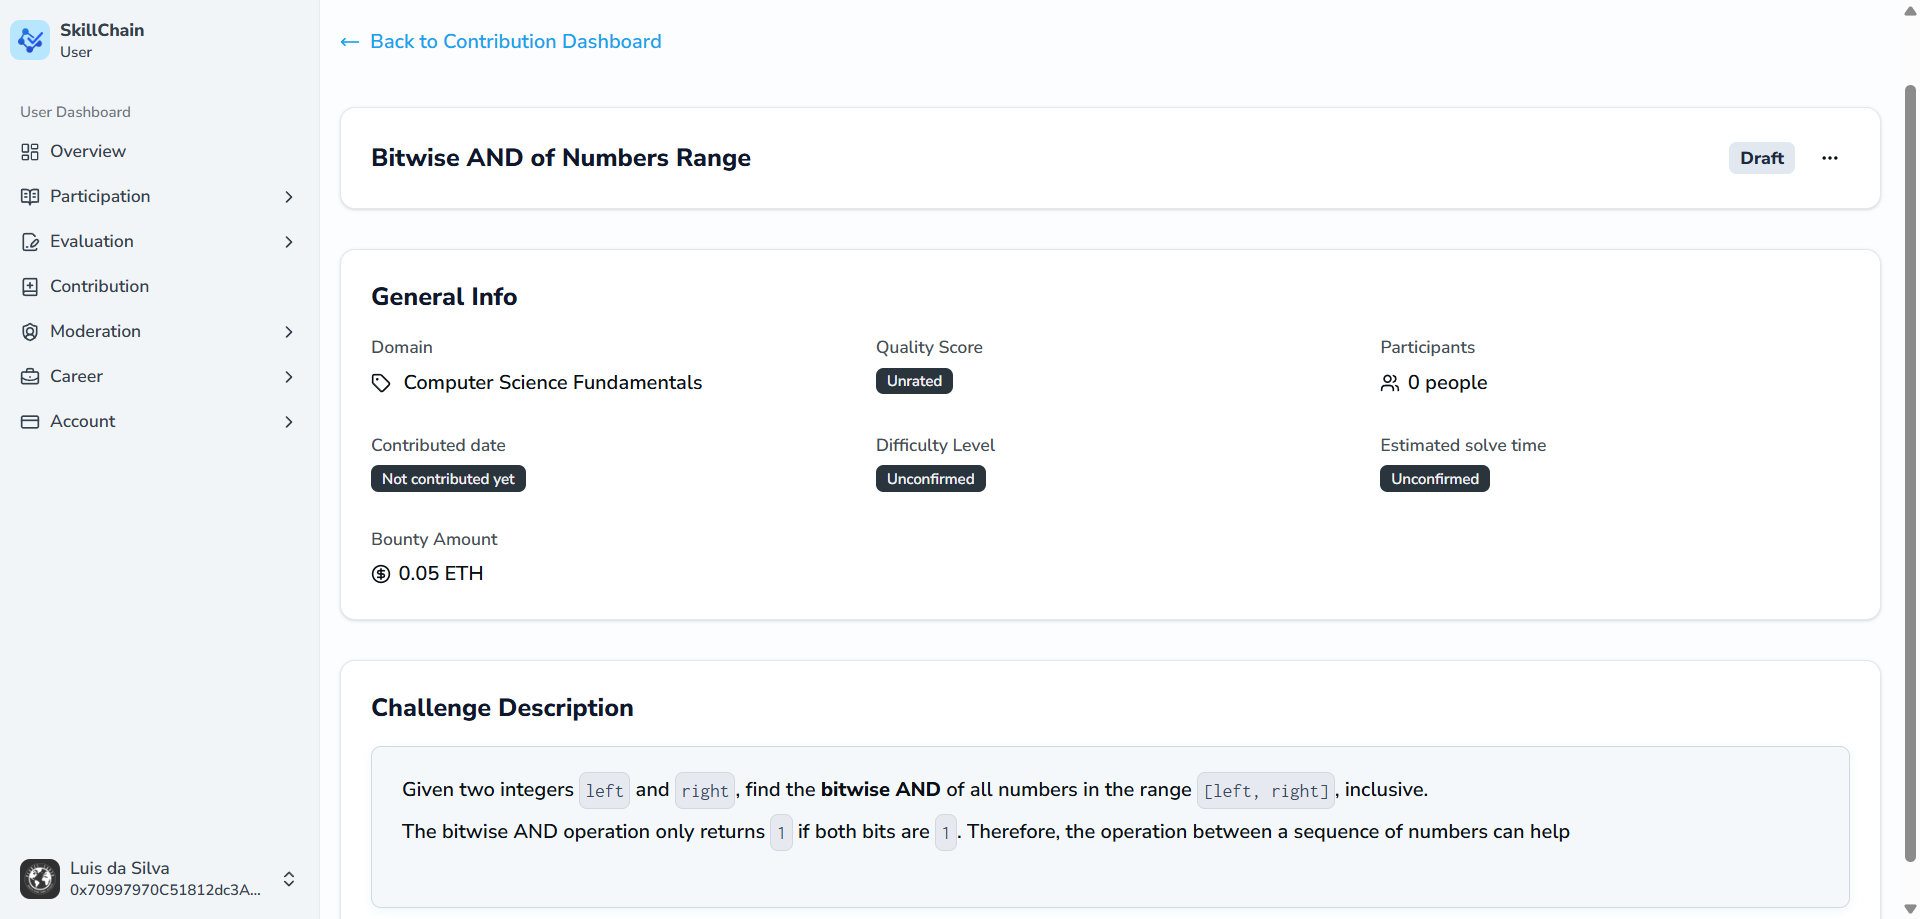
\includegraphics[width=0.99\textwidth, frame]{ui/contribution-challenge-detail-page.png}
  \caption{Trang chi tiết thử thách đã tạo}
  \label{fig:contribution-challenge-detail-page}
\end{figure}

\begin{figure}[H]
  \centering
  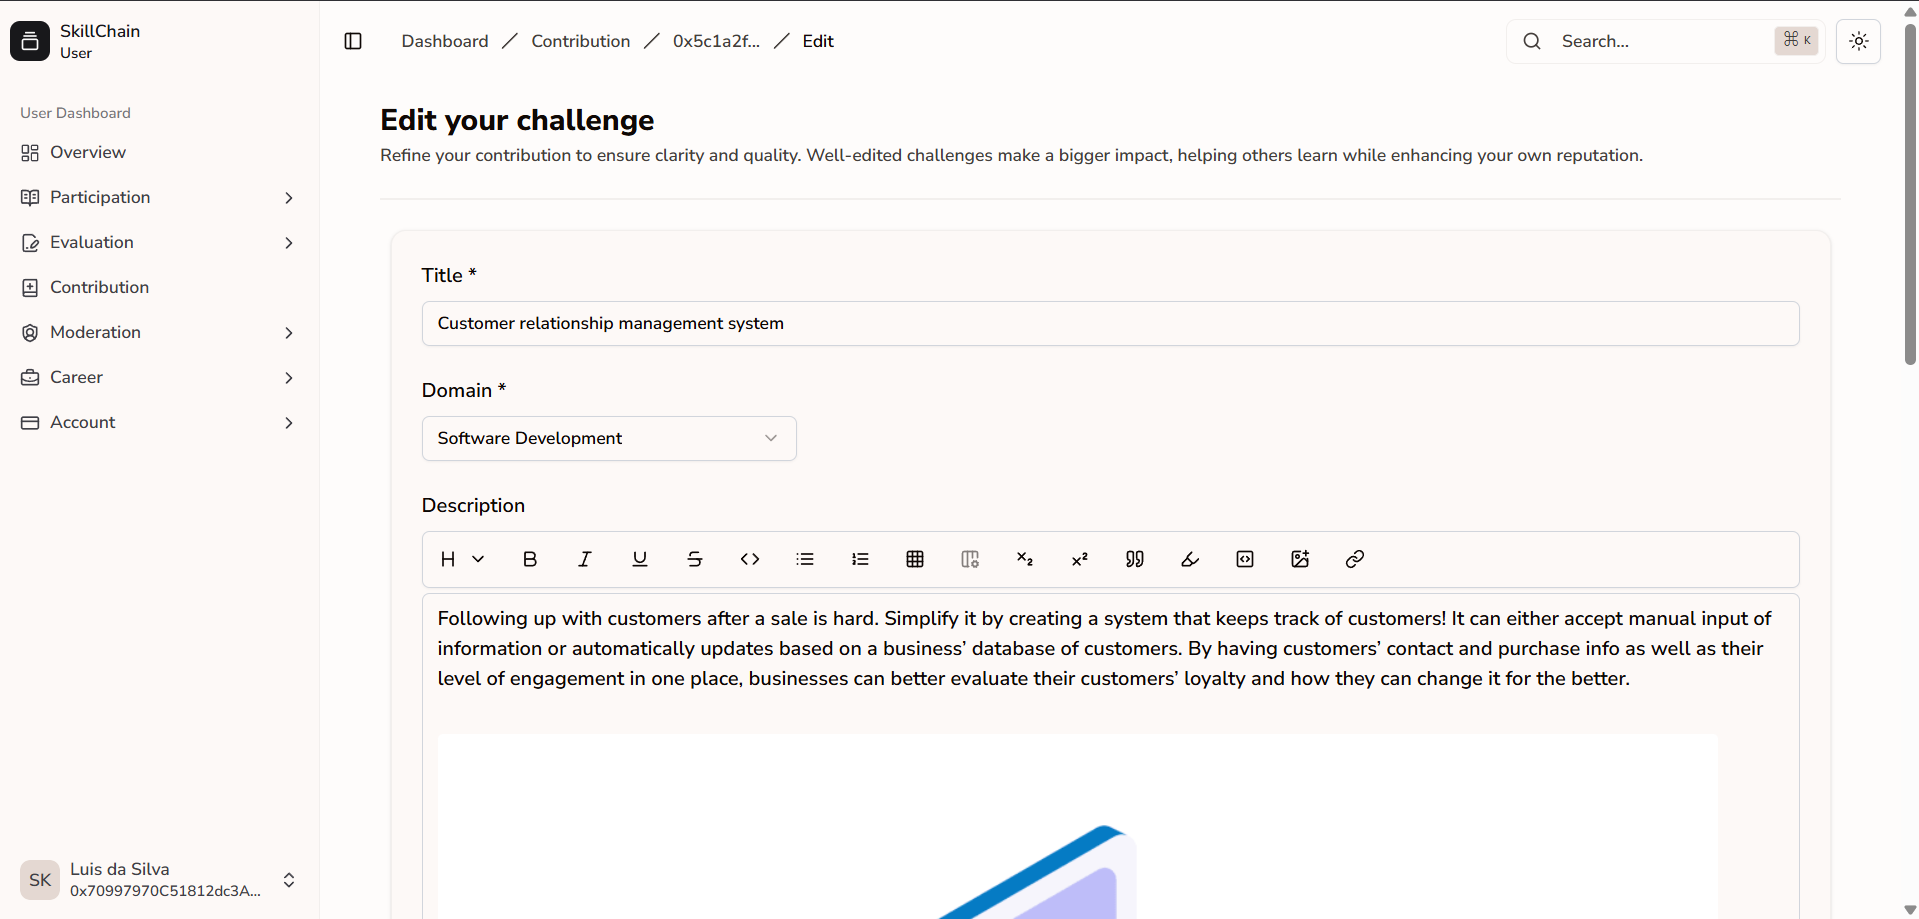
\includegraphics[width=0.99\textwidth, frame]{ui/contribution-challenge-edit-page.png}
  \caption{Trang chỉnh sửa thử thách}
  \label{fig:contribution-challenge-edit-page}
\end{figure}

Người dùng có thể chỉnh sửa nội dung thử thách tại đây và nhấn ``Save changes'' để lưu thay đổi.

\subsubsection{Gửi thử thách cho kiểm duyệt}

Để gửi thử thách đến bên kiểm duyệt, người dùng truy cập trang chi tiết của thử thách và nhấn nút ``Contribute''.  
Hệ thống sẽ yêu cầu xác thực giao dịch thông qua ví tiền điện tử để chính thức chuyển thử thách sang trạng thái chờ kiểm duyệt.  
Sau khi gửi đi, thử thách sẽ bị khóa và không còn có thể chỉnh sửa được nữa.

\subsection{Kiểm duyệt thử thách}

\subsubsection{Xem thử thách chờ kiểm duyệt}

Để xem danh sách các thử thách đang chờ kiểm duyệt, người dùng truy cập \textbf{Moderation} $\rightarrow$ \textbf{Pending Challenge}.  
Tại đây, người dùng có thể xem thông tin chi tiết từng thử thách, bao gồm số lượng người đã tham gia kiểm duyệt.

\begin{figure}[H]
  \centering
  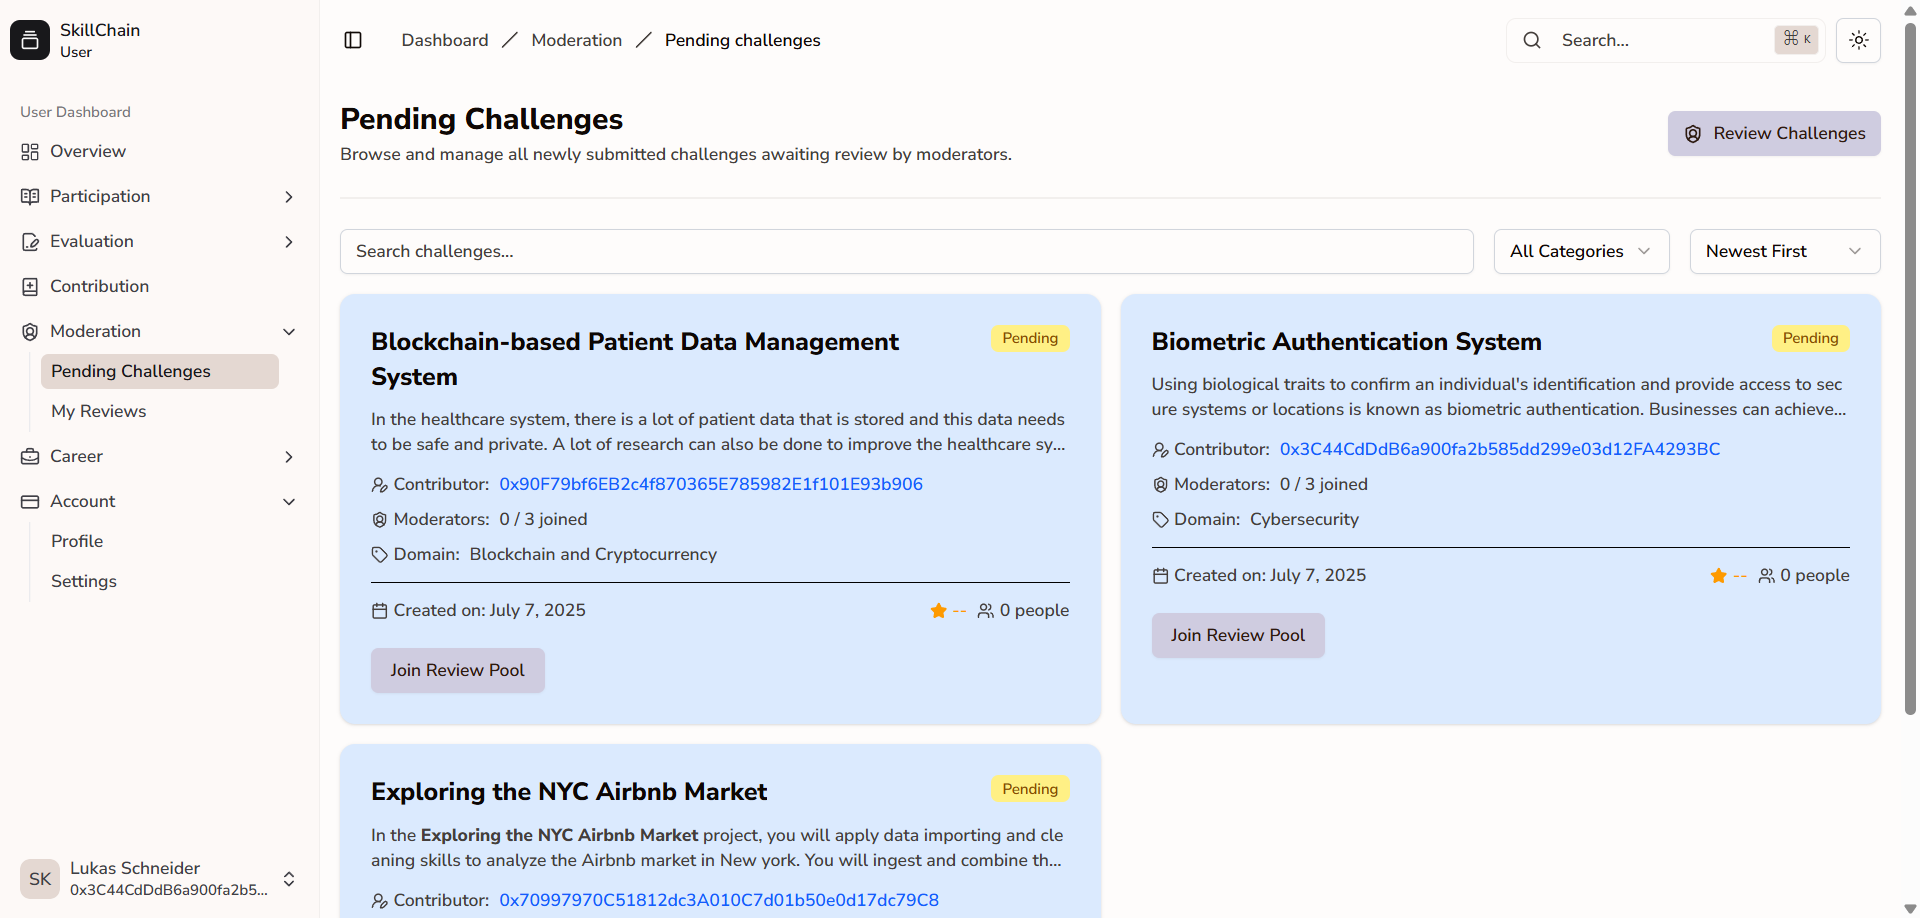
\includegraphics[width=0.99\textwidth, frame]{ui/moderation-pending-challenges-page.png}
  \caption{Trang danh sách thử thách chờ kiểm duyệt}
  \label{fig:moderation-pending-challenges-page}
\end{figure}

\subsubsection{Tham gia kiểm duyệt thử thách}

Để tham gia kiểm duyệt một thử thách, người dùng nhấn nút ``Join Review Pool'' tại thử thách mong muốn.  
Hệ thống sẽ yêu cầu xác thực giao dịch thông qua ví tiền điện tử để hoàn tất việc tham gia kiểm duyệt.
Nếu người dùng không đủ chỉ số uy tín chuyên môn tương ứng với loại thử thách, hệ thống sẽ hiển thị thông báo lỗi và không cho phép tham gia.

\subsubsection{Thực hiện kiểm duyệt}

Để bắt đầu kiểm duyệt, người dùng truy cập \textbf{Moderation} $\rightarrow$ \textbf{My Reviews} để xem danh sách các thử thách mà mình đã tham gia kiểm duyệt.  
Sau đó, chọn thử thách tương ứng và nhấn nút ``Edit review''.

\begin{figure}[H]
  \centering
  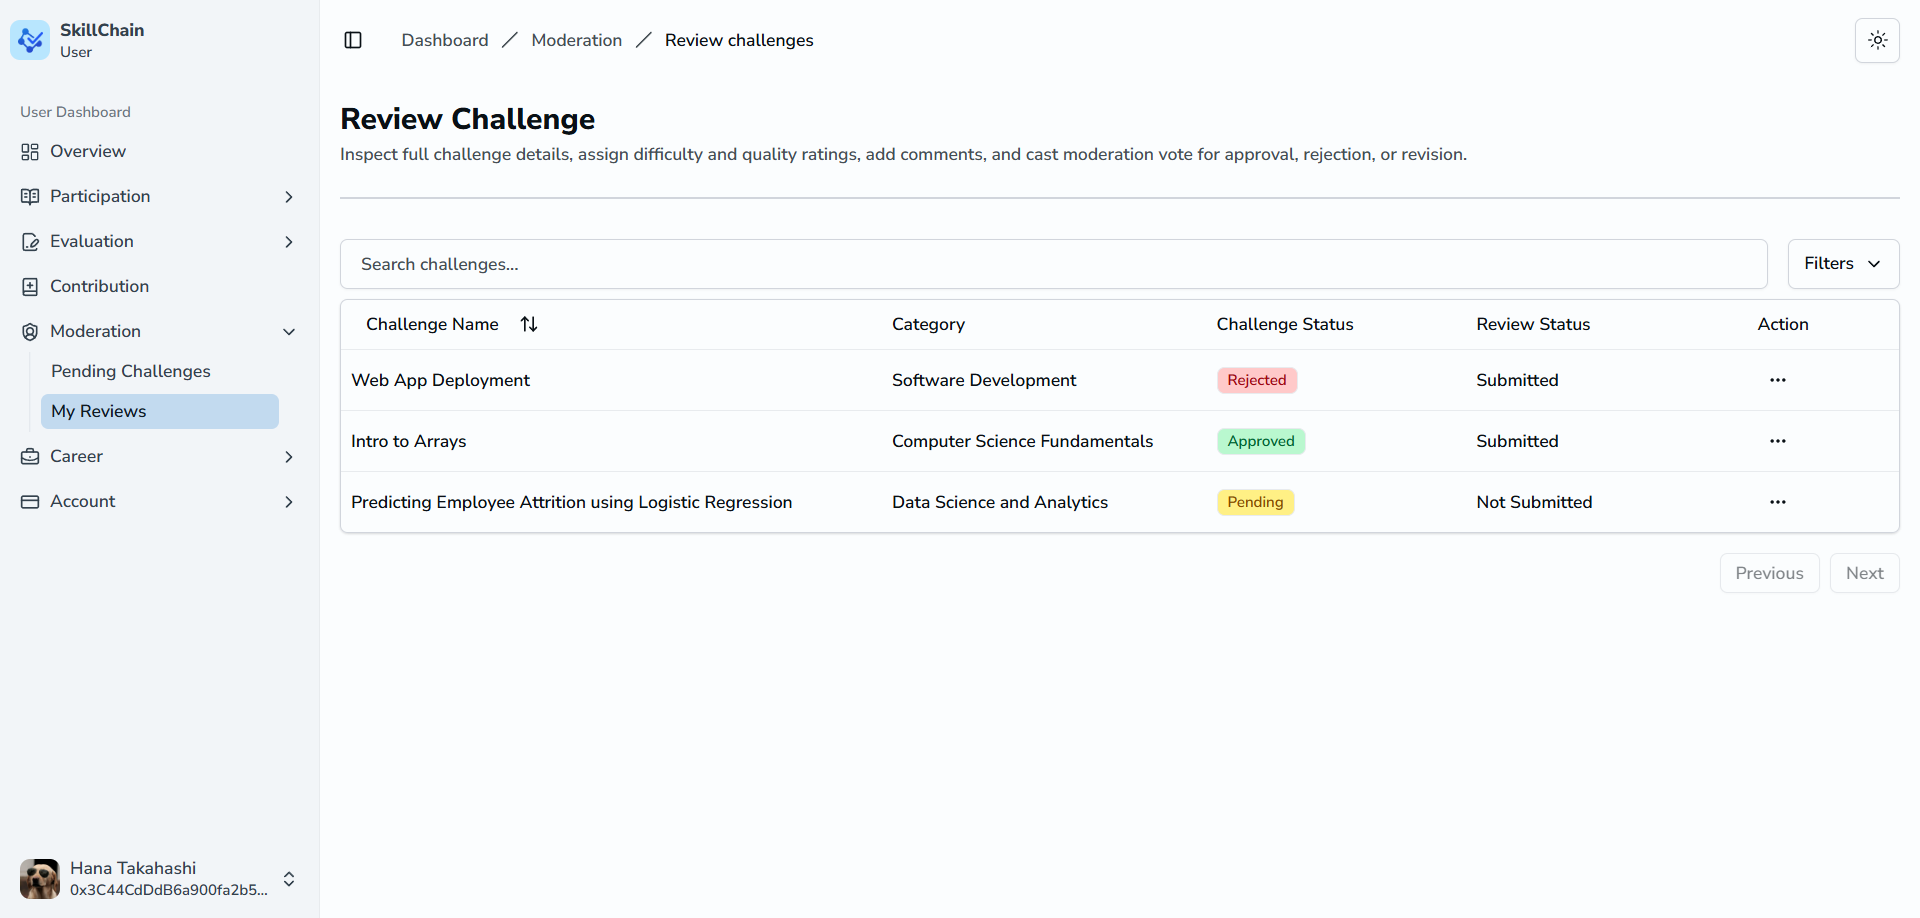
\includegraphics[width=0.99\textwidth, frame]{ui/moderation-my-reviews-page.png}
  \caption{Trang danh sách thử thách đã và đang kiểm duyệt}
  \label{fig:moderation-my-reviews-page}
\end{figure}

Tại trang này, người dùng có thể xem chi tiết phiên kiểm duyệt.  
Để thực hiện đánh giá, chuyển sang tab \textbf{Review Form}.

Trong biểu mẫu kiểm duyệt, người dùng cần:
\begin{itemize}
  \item Chọn \textbf{Yes/No} cho từng tiêu chí đánh giá chất lượng.
  \item Đề xuất độ khó và thời gian giải ước tính.
  \item Có thể lưu tạm nội dung đánh giá hoặc gửi luôn.
\end{itemize}

Sau khi hoàn tất, nhấn nút ``Submit Review'' để nộp đánh giá.  
Giao dịch sẽ cần được xác thực qua ví tiền điện tử, và sau khi gửi, nội dung đánh giá sẽ không thể chỉnh sửa.

\begin{figure}[H]
  \centering
  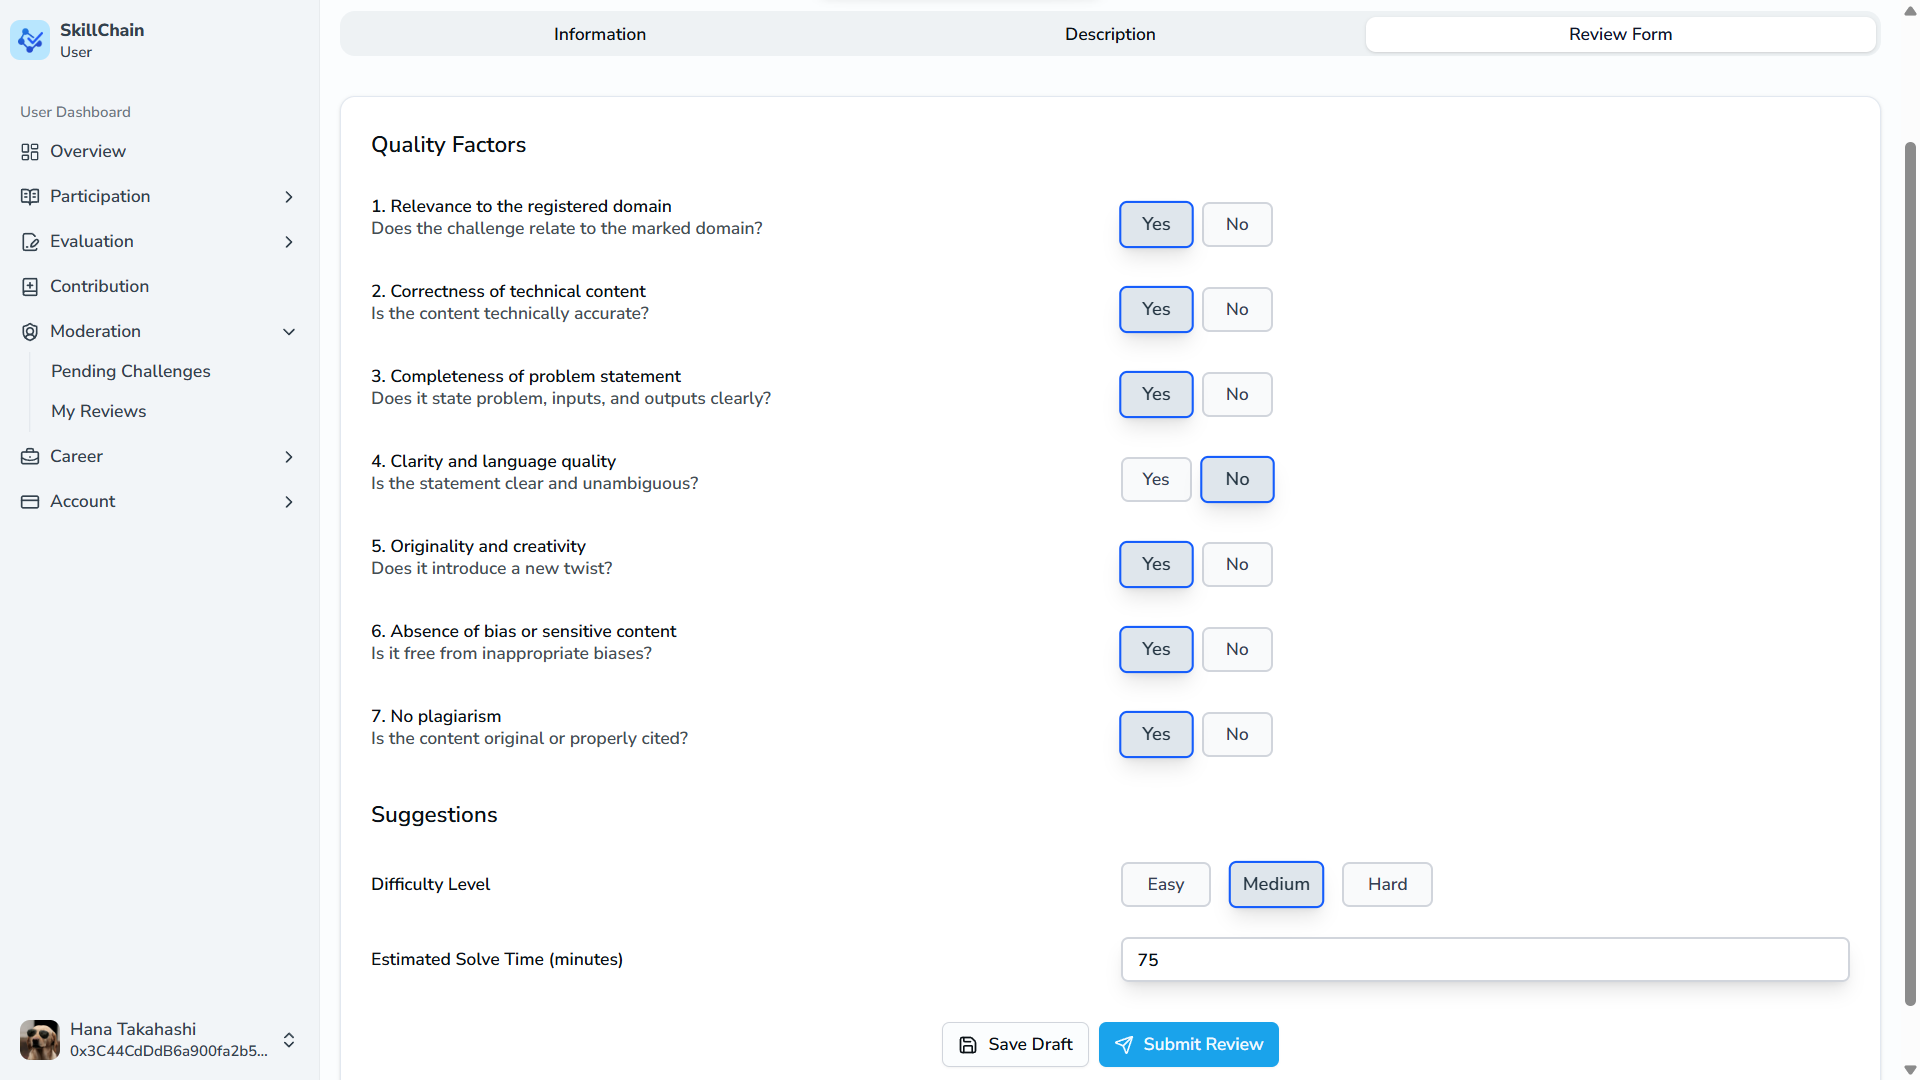
\includegraphics[width=0.99\textwidth, frame]{ui/moderation-review-form.png}
  \caption{Biểu mẫu kiểm duyệt chất lượng thử thách}
  \label{fig:moderation-review-form}
\end{figure}

\subsubsection{Xem thông tin phiên kiểm duyệt}

Khi phiên kiểm duyệt kết thúc, thông tin chi tiết về phiên sẽ được hiển thị cho người đóng góp và các kiểm duyệt viên.  
Thông tin này bao gồm danh sách người kiểm duyệt, số điểm đánh giá, và phần token thưởng tương ứng.

\begin{figure}[H]
  \centering
  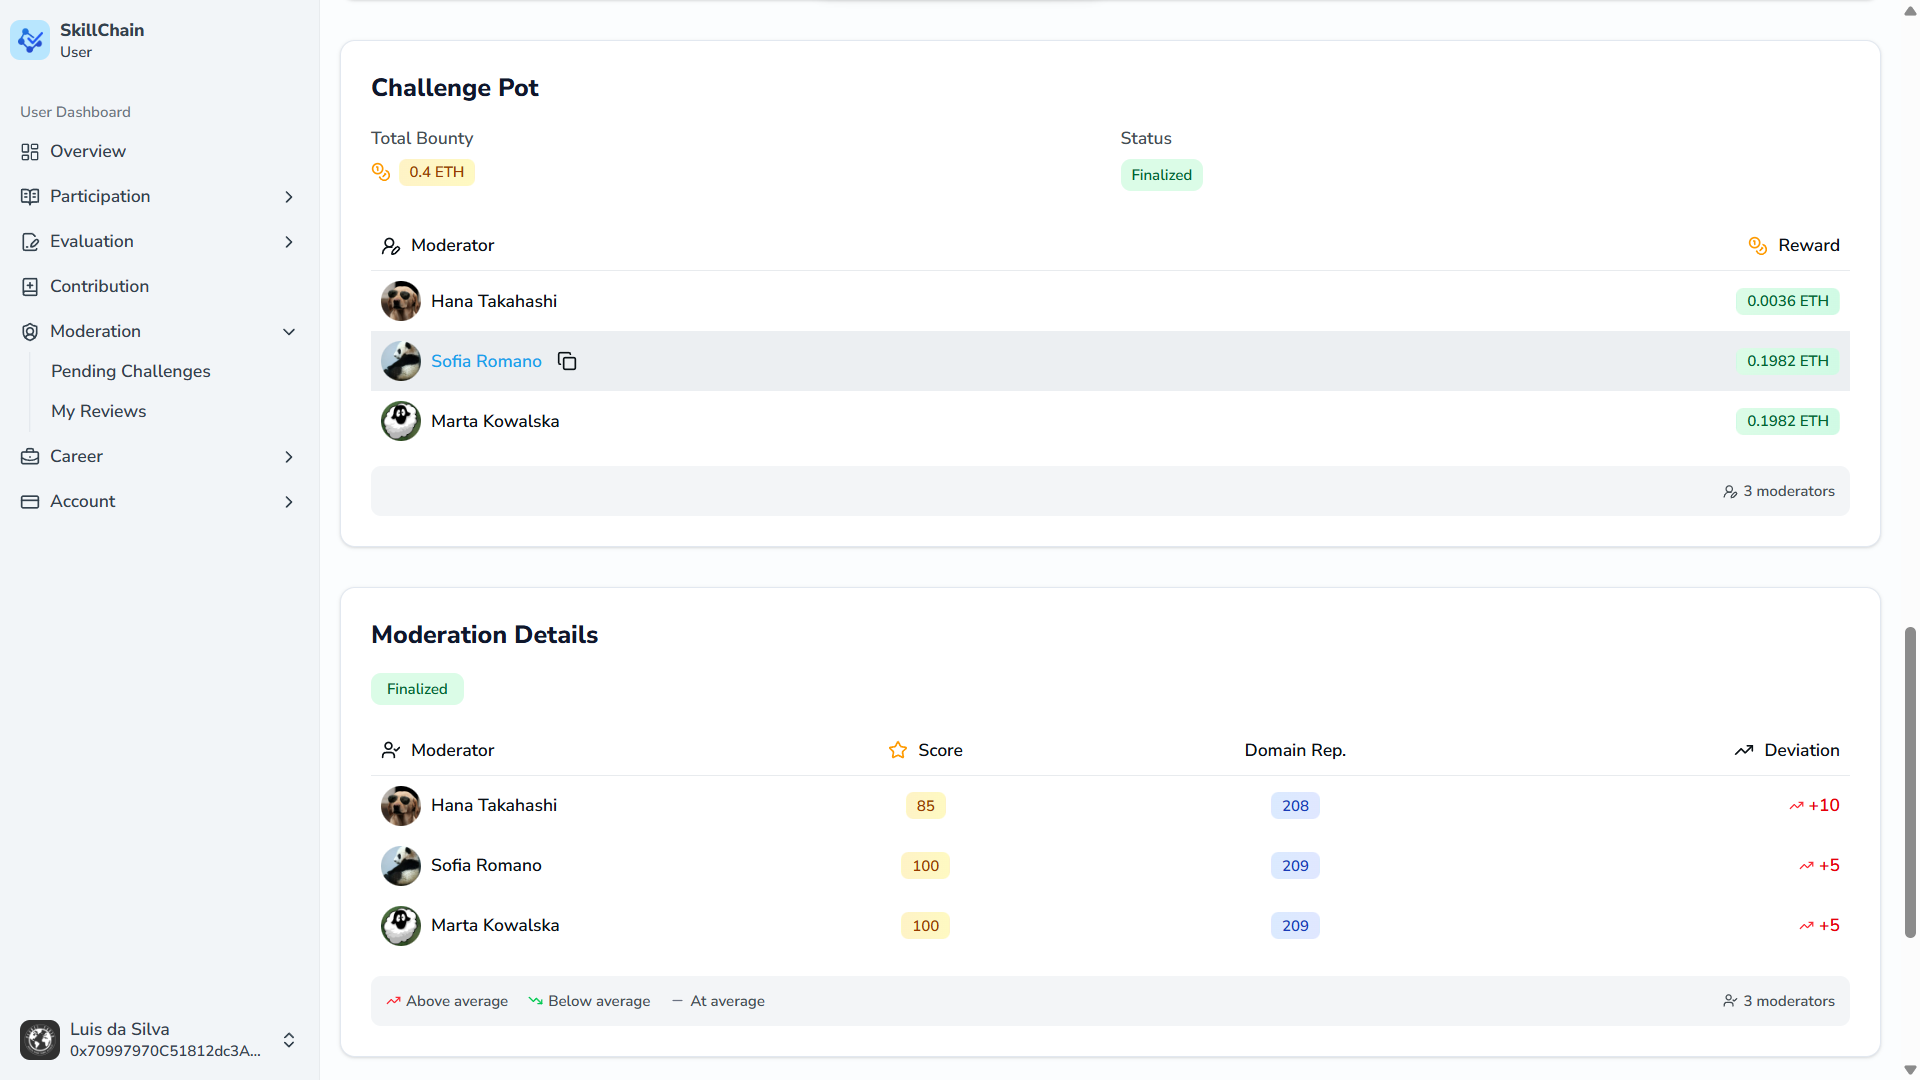
\includegraphics[width=0.99\textwidth, frame]{ui/challenge-moderation-pot-info.png}
  \caption{Thông tin chi tiết của một phiên kiểm duyệt}
  \label{fig:challenge-moderation-pot-info}
\end{figure}

\subsection{Tham gia thử thách}

\subsubsection{Xem thử thách đang hiện hành}

Để xem danh sách các thử thách đang mở, người dùng truy cập \textbf{Participation} $\rightarrow$ \textbf{Explore}.  
Tại đây, người dùng có thể xem chi tiết nội dung từng thử thách bằng cách nhấn vào thẻ tương ứng.

\begin{figure}[H]
  \centering
  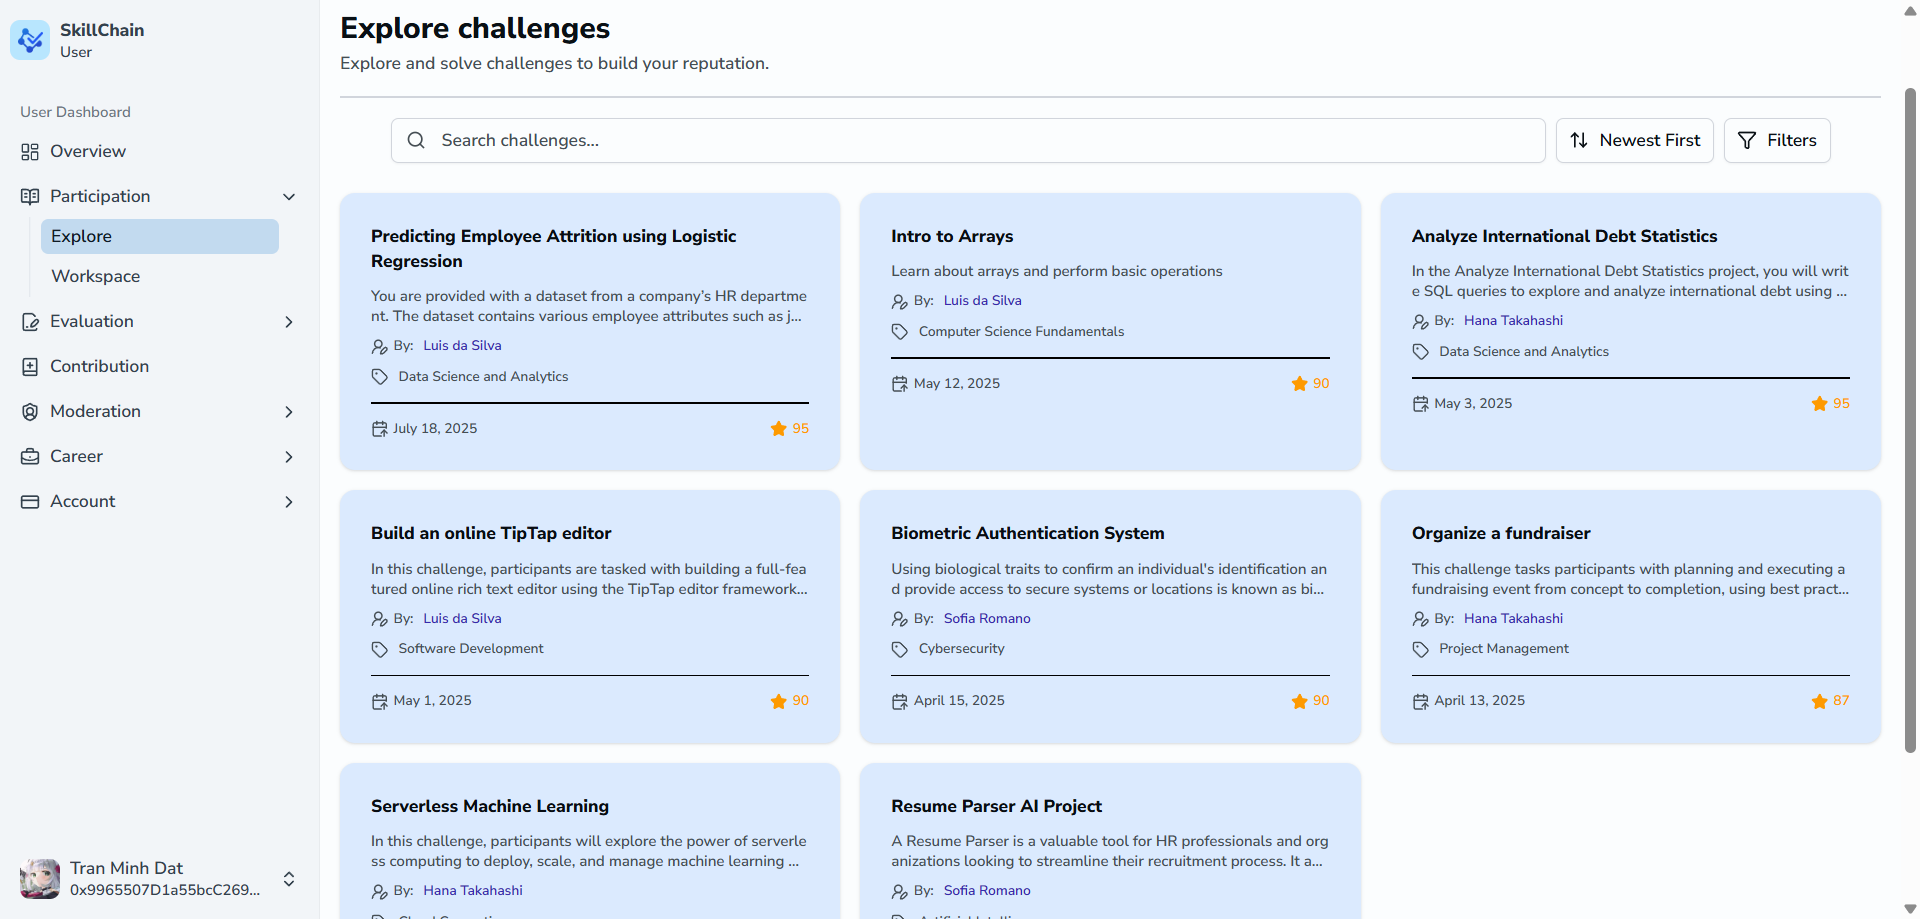
\includegraphics[width=0.99\textwidth, frame]{ui/explore-challenges-page.png}
  \caption{Trang danh sách thử thách đang hiện hành}
  \label{fig:explore-challenges-page}
\end{figure}

\subsubsection{Thực hiện thử thách}

Khi xem chi tiết nội dung một thử thách, người dùng có thể nhấn nút ``Join Challenge'' (ở góc trên hoặc góc dưới bên phải) để tham gia.  
Hệ thống sẽ yêu cầu người dùng xác nhận trả một khoản phí và xác thực giao dịch qua ví tiền điện tử.

\begin{figure}[H]
  \centering
  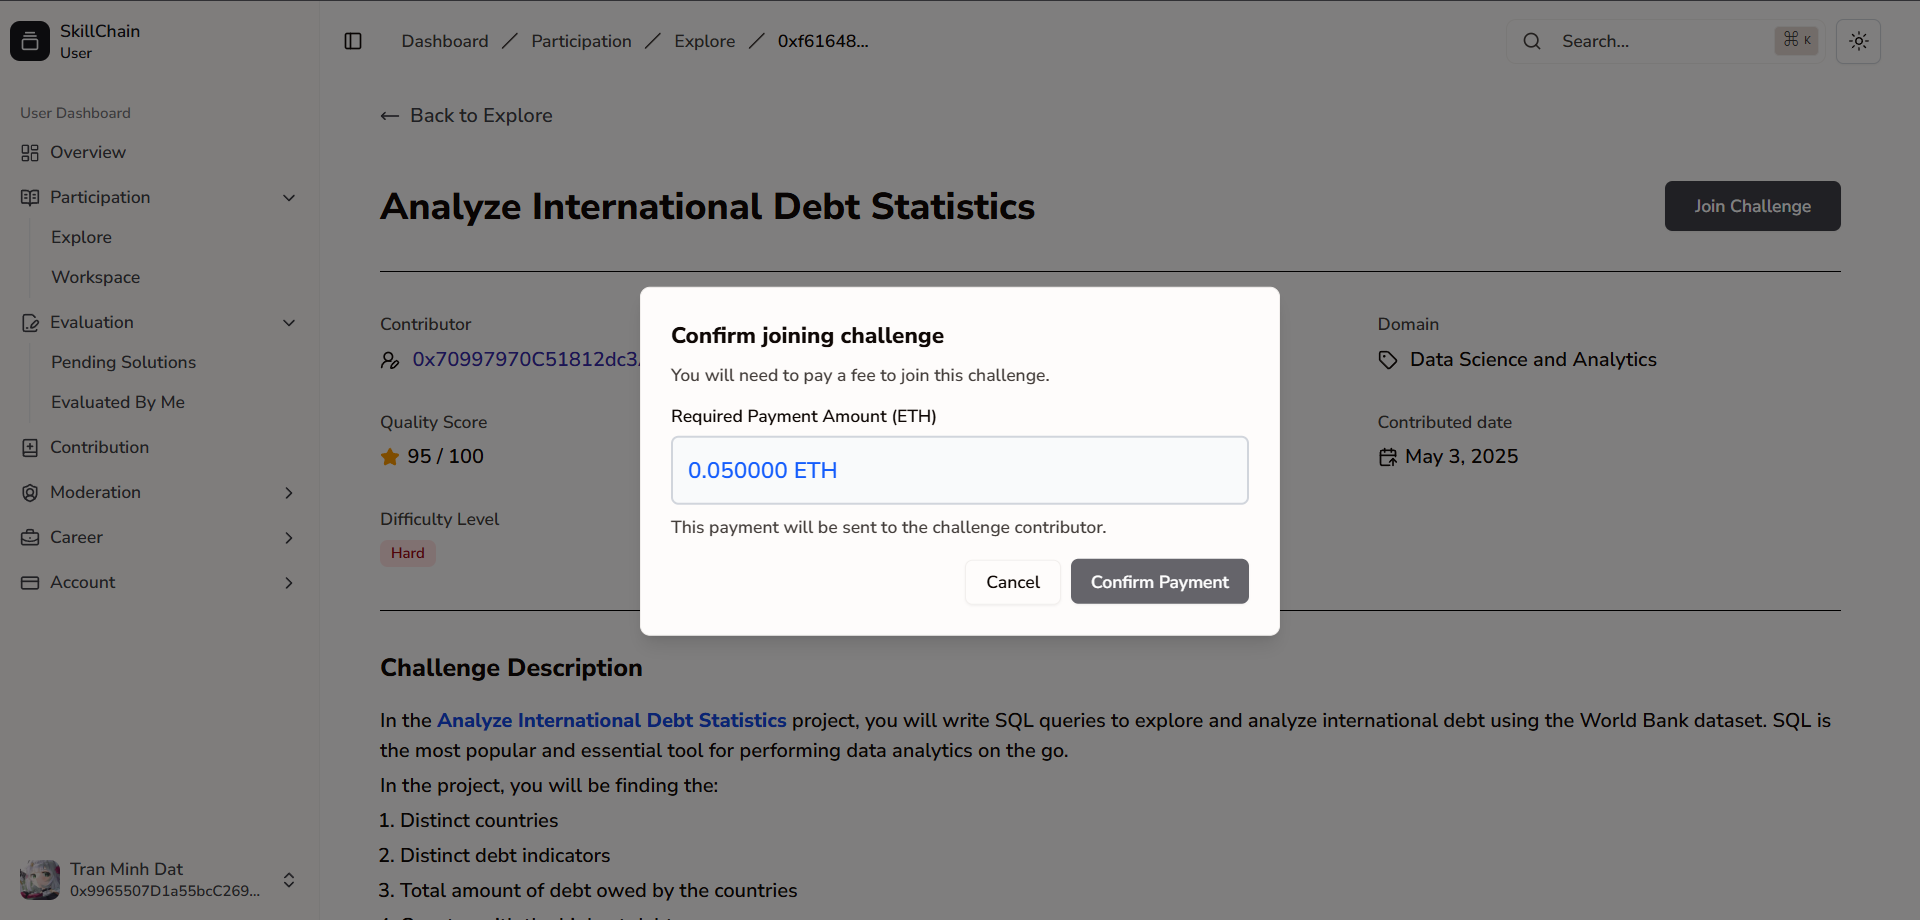
\includegraphics[width=0.99\textwidth, frame]{ui/join-challenge-payment-dialog.png}
  \caption{Xác nhận trả phí tham gia thử thách}
  \label{fig:join-challenge-payment-dialog}
\end{figure}

Sau khi tham gia thành công, người dùng truy cập \textbf{Participation} $\rightarrow$ \textbf{Workspace} để xem các thử thách đã và đang tham gia.  
Tại đây, người dùng có thể bắt đầu xây dựng giải pháp. Hệ thống cho phép lưu tạm giải pháp nhiều lần trước khi nộp chính thức.

\begin{figure}[H]
  \centering
  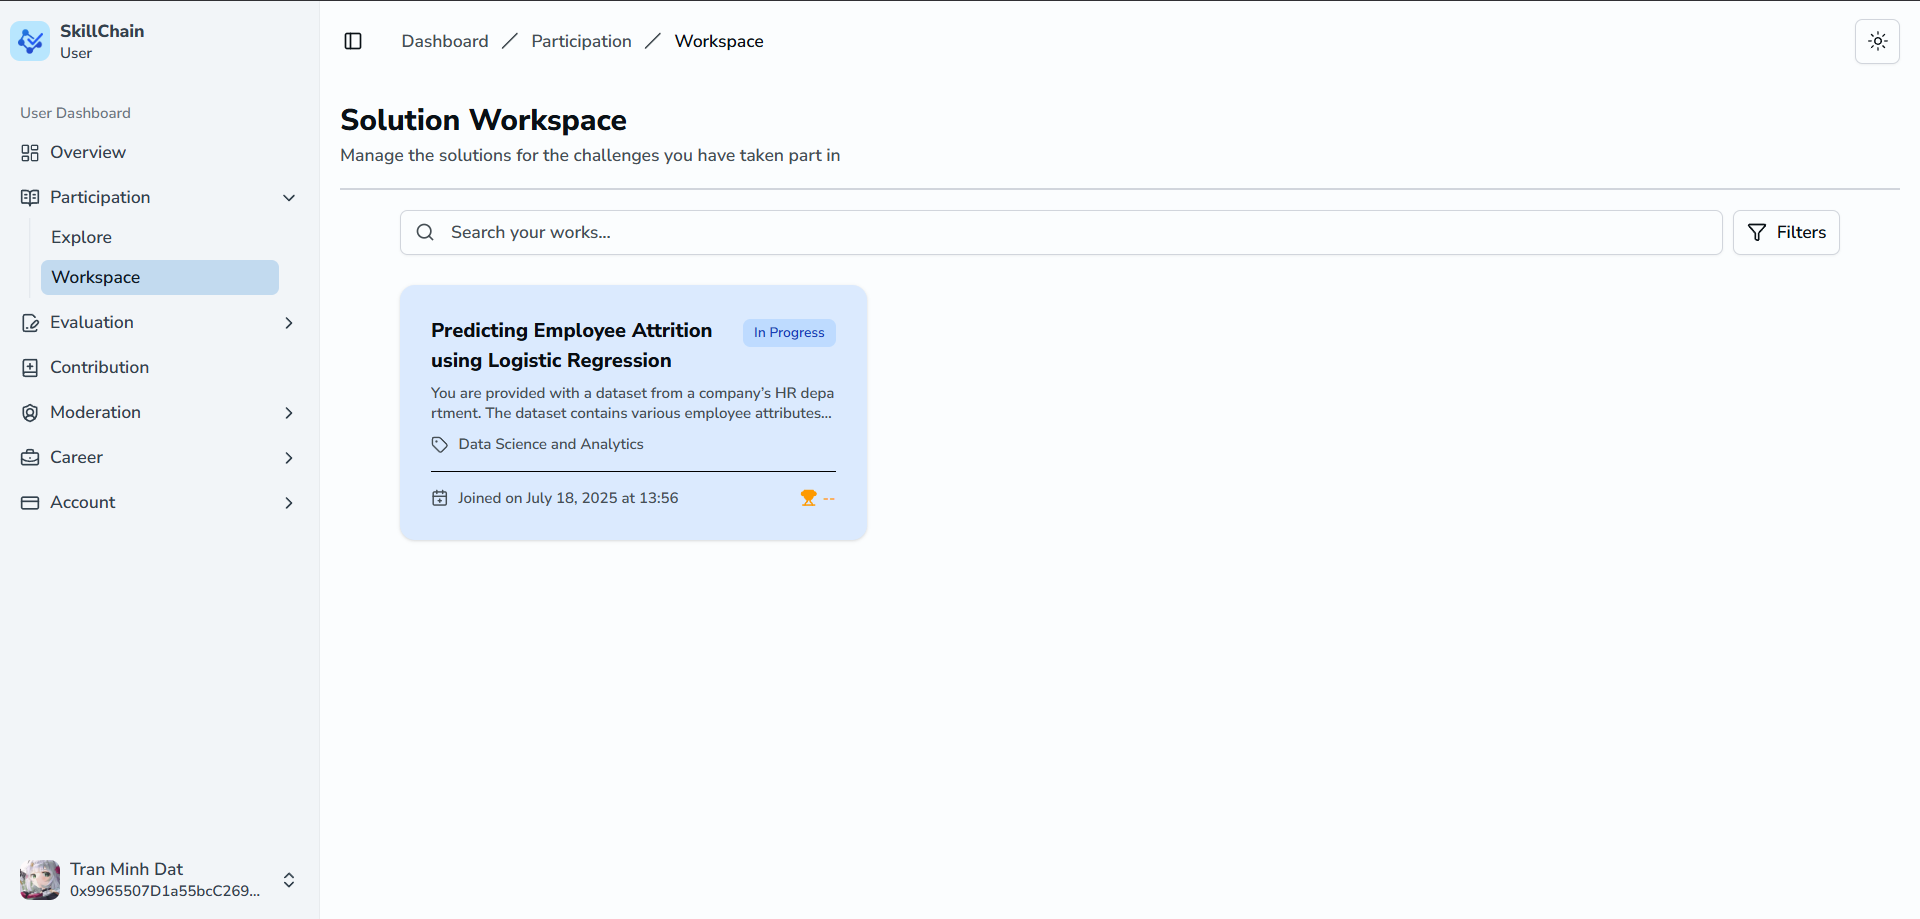
\includegraphics[width=0.99\textwidth, frame]{ui/workspace-challenge-page.png}
  \caption{Trang danh sách thử thách đã tham gia}
  \label{fig:workspace-challenge-page}
\end{figure}

\begin{figure}[H]
  \centering
  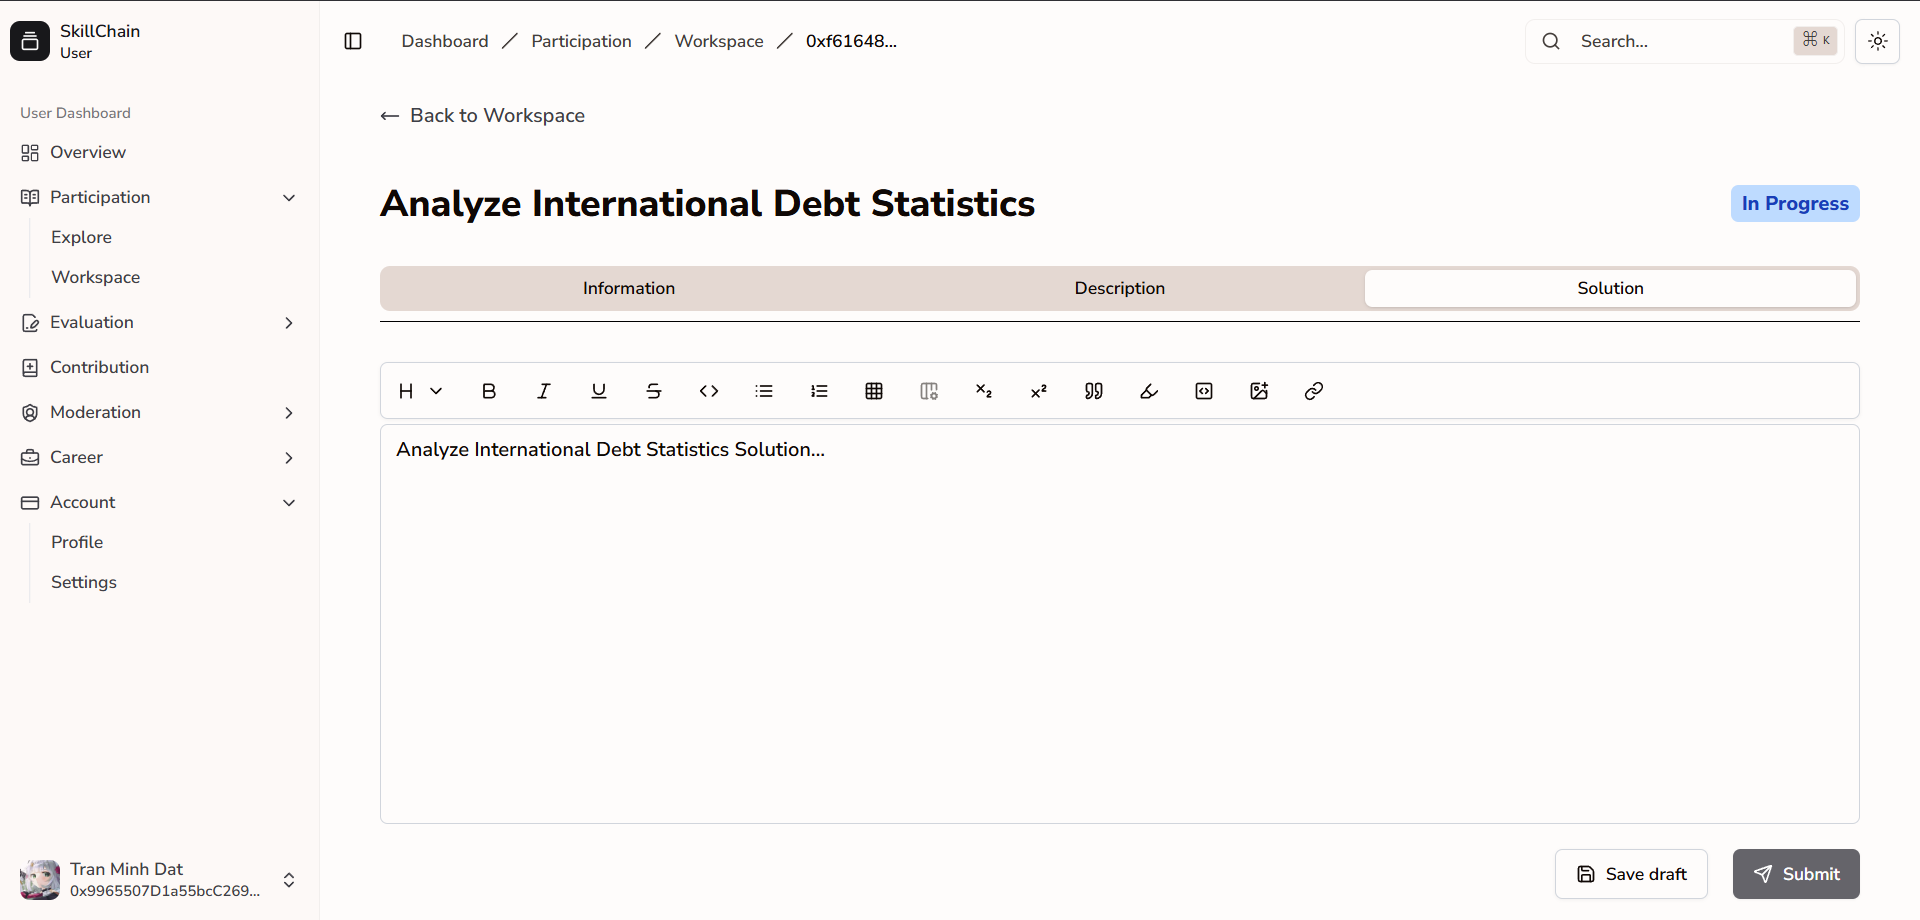
\includegraphics[width=0.99\textwidth, frame]{ui/solution-workspace-page.png}
  \caption{Không gian soạn thảo giải pháp}
  \label{fig:solution-workspace-page}
\end{figure}

Sau khi hoàn thiện giải pháp, người dùng nhấn nút ``Submit'' để nộp bài. Kể từ thời điểm này, nội dung giải pháp sẽ bị khóa và không thể chỉnh sửa.
Khi đã sẵn sàng gửi bài để chấm điểm, người dùng nhấn ``Put Under Review''. Mỗi hành động nộp bài hoặc gửi đánh giá đều yêu cầu xác thực giao dịch thông qua ví tiền điện tử.

\begin{figure}[H]
  \centering
  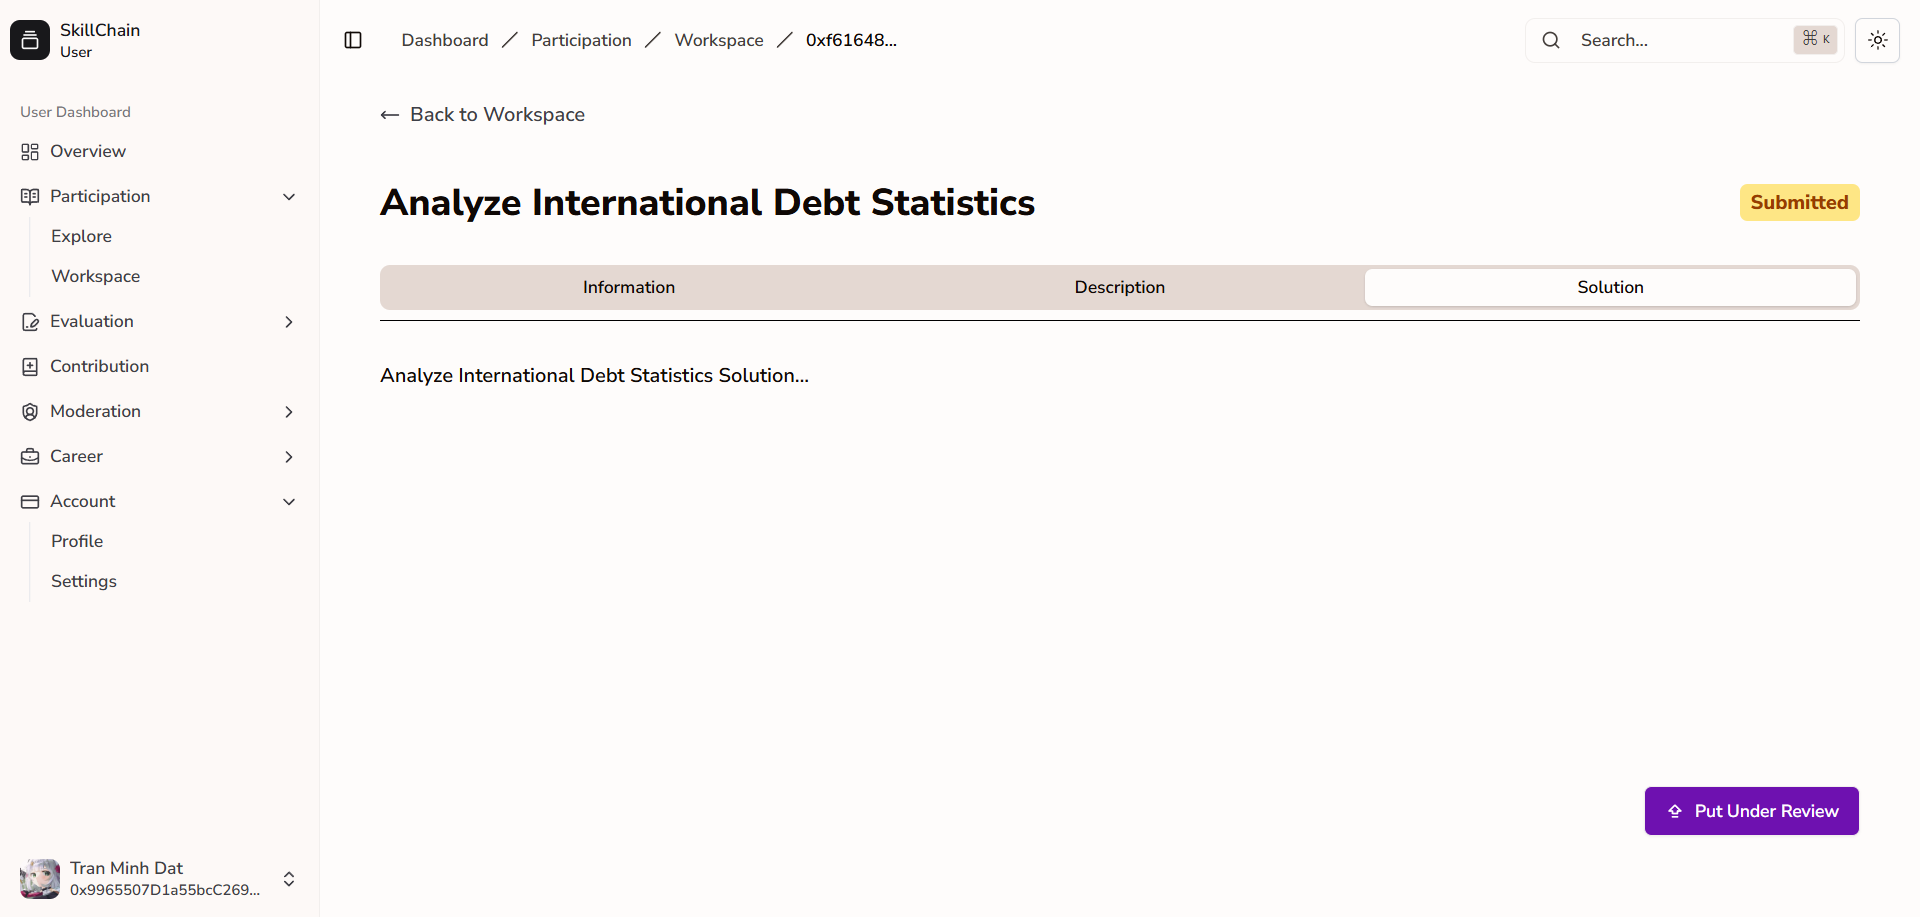
\includegraphics[width=0.99\textwidth, frame]{ui/submitted-solution-page.png}
  \caption{Giải pháp đã được nộp}
  \label{fig:submitted-solution-page}
\end{figure}

\subsection{Đánh giá giải pháp}

\subsubsection{Xem giải pháp đang chờ đánh giá}

Để xem danh sách các giải pháp đang chờ đánh giá, người dùng truy cập \textbf{Evaluation} $\rightarrow$ \textbf{Pending Solution}.  
Tại đây, hệ thống hiển thị các giải pháp đang chờ đánh giá, bao gồm tên người nộp giải, số lượng người đánh giá đã tham gia.  
Tuy nhiên, nội dung chi tiết của giải pháp sẽ chưa được hiển thị ở giai đoạn này.

\begin{figure}[H]
  \centering
  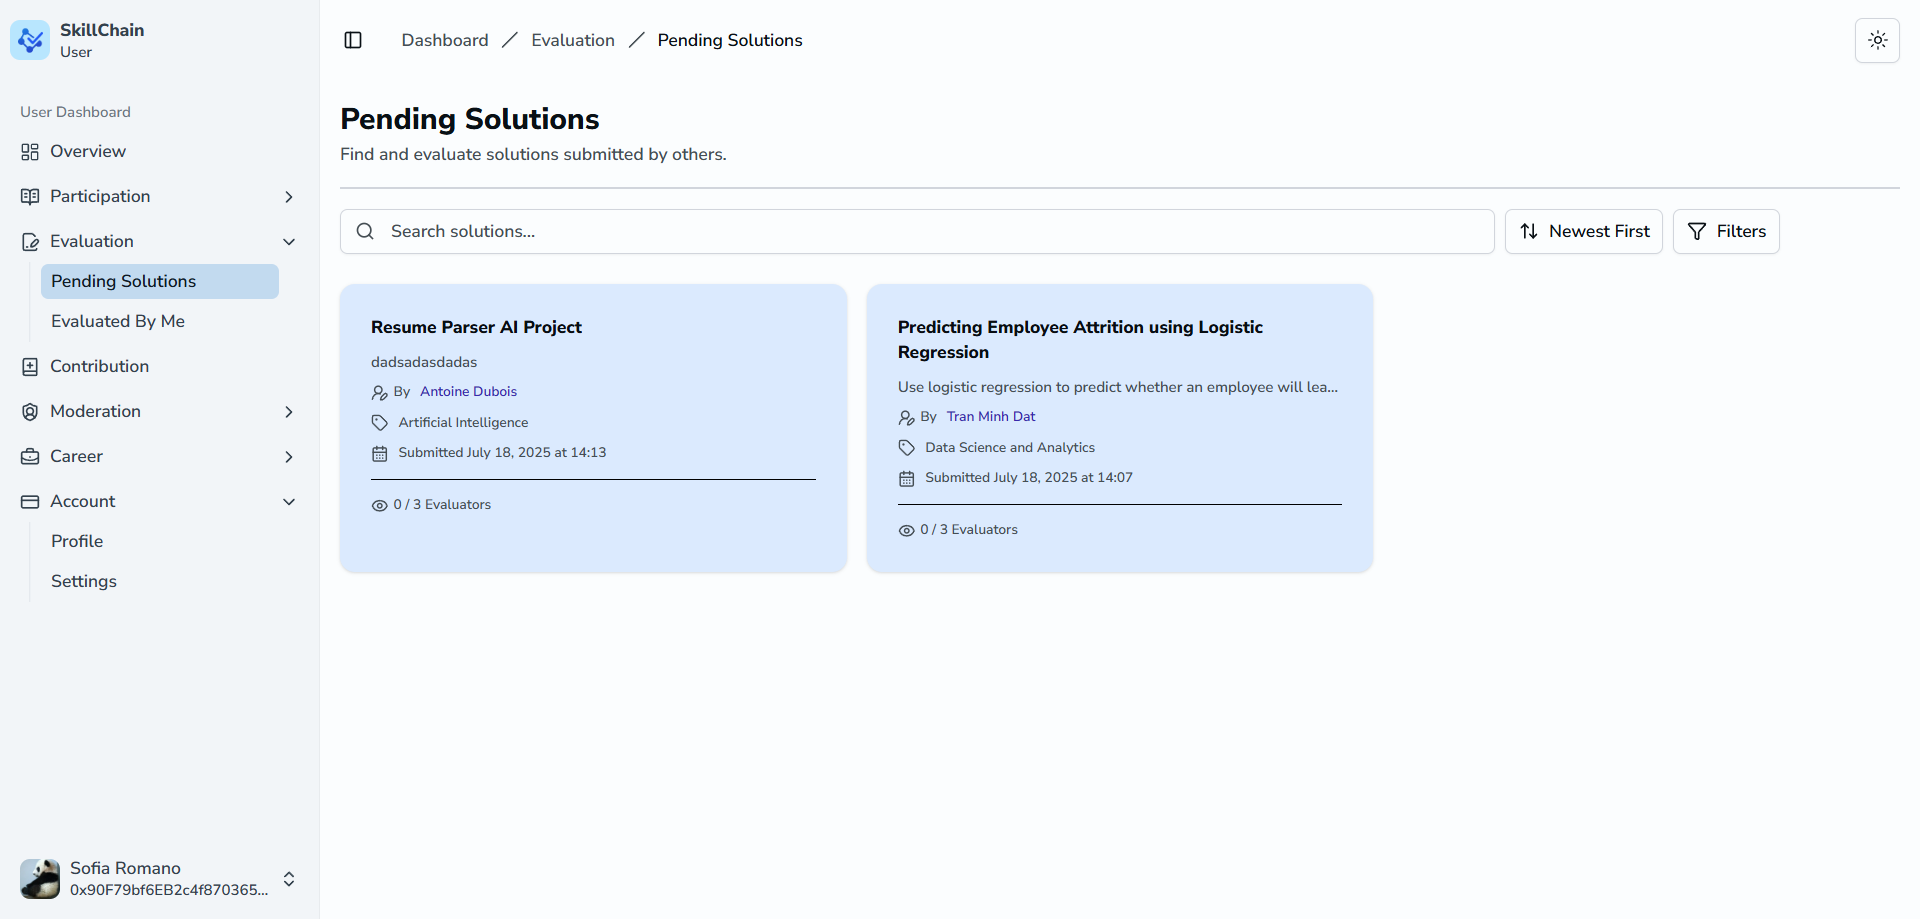
\includegraphics[width=0.99\textwidth, frame]{ui/pending-solution-page.png}
  \caption{Trang danh sách giải pháp đang chờ đánh giá}
  \label{fig:pending-solution-page}
\end{figure}

\subsubsection{Tham gia đánh giá giải pháp}

Khi xem thông tin chi tiết của một giải pháp, người dùng có thể nhấn nút ``Evaluate Solution'' để đăng ký tham gia đánh giá.  
Hệ thống sẽ yêu cầu xác thực giao dịch thông qua ví tiền điện tử để xác nhận quyền đánh giá.
Nếu người dùng không đủ chỉ số uy tín chuyên môn phù hợp với loại thử thách, hệ thống sẽ hiển thị thông báo lỗi và không cho phép tiếp tục.

\begin{figure}[H]
  \centering
  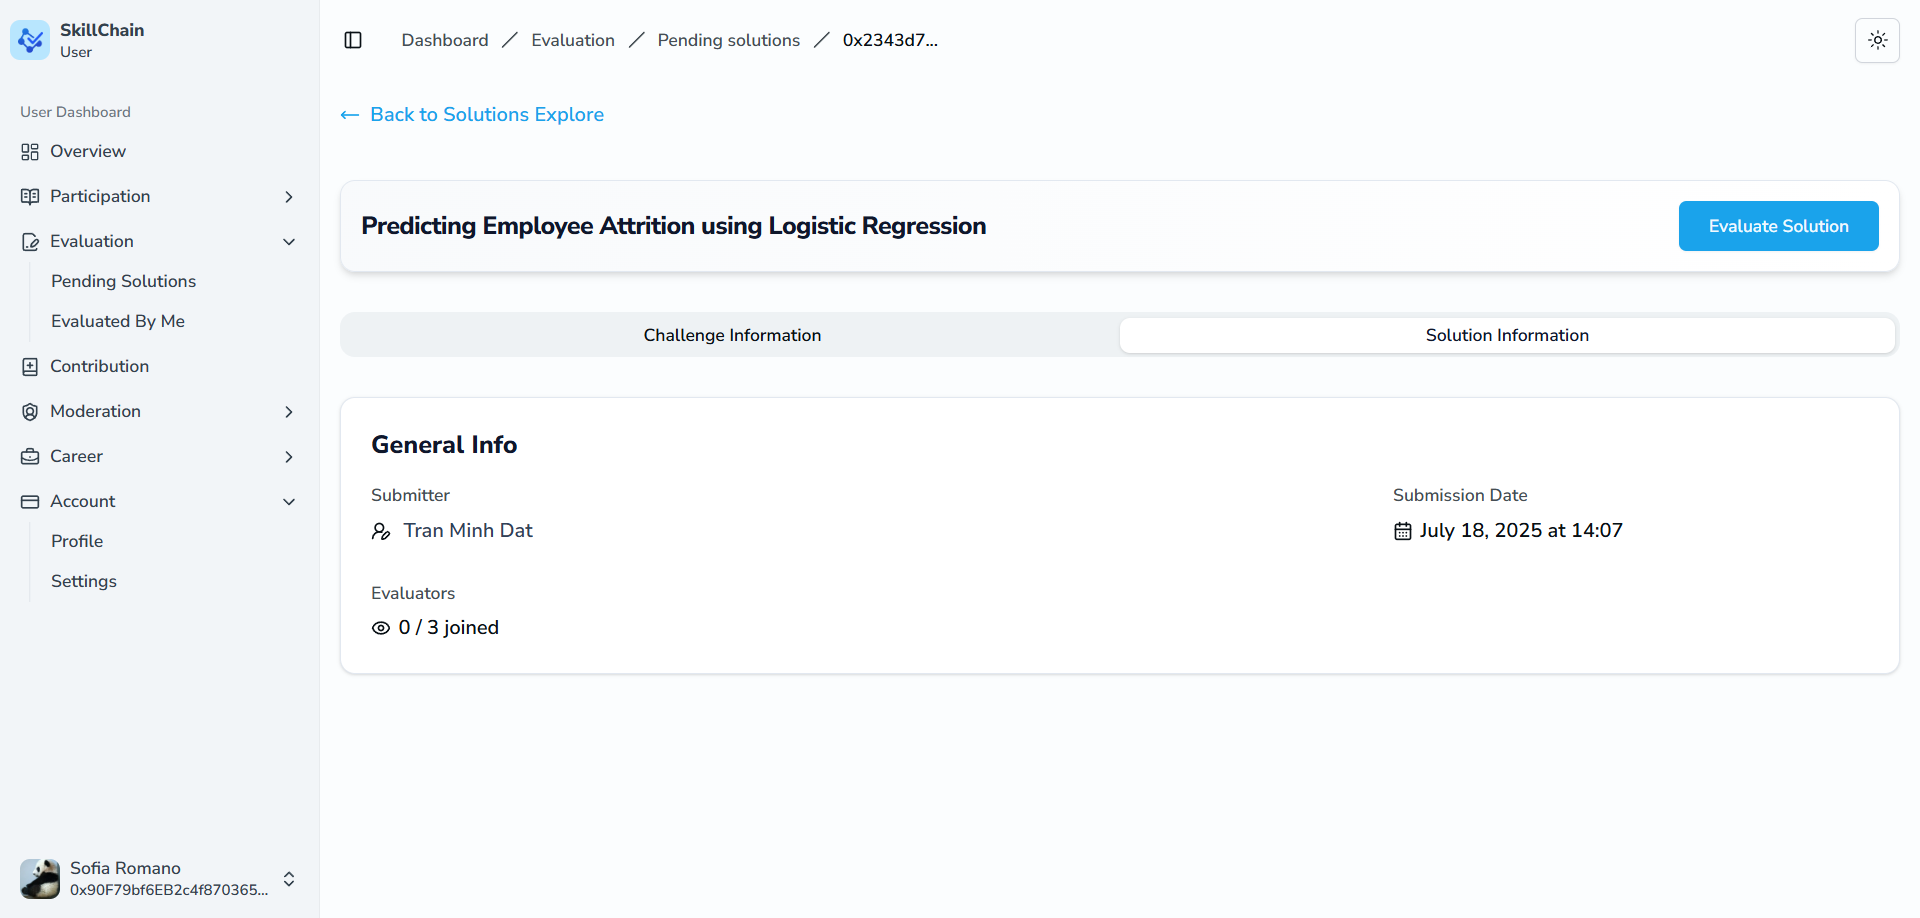
\includegraphics[width=0.99\textwidth, frame]{ui/pending-solution-info-page.png}
  \caption{Thông tin cơ bản của giải pháp đang chờ đánh giá}
  \label{fig:pending-solution-info-page}
\end{figure}

\subsubsection{Thực hiện đánh giá giải pháp}

Sau khi tham gia đánh giá, người dùng truy cập \textbf{Evaluation} $\rightarrow$ \textbf{Evaluated By Me} để xem danh sách các giải pháp mà mình đã hoặc đang đánh giá.  
Tại đây, người đánh giá có thể xem nội dung chi tiết của giải pháp và tiến hành chấm điểm.

\begin{figure}[H]
  \centering
  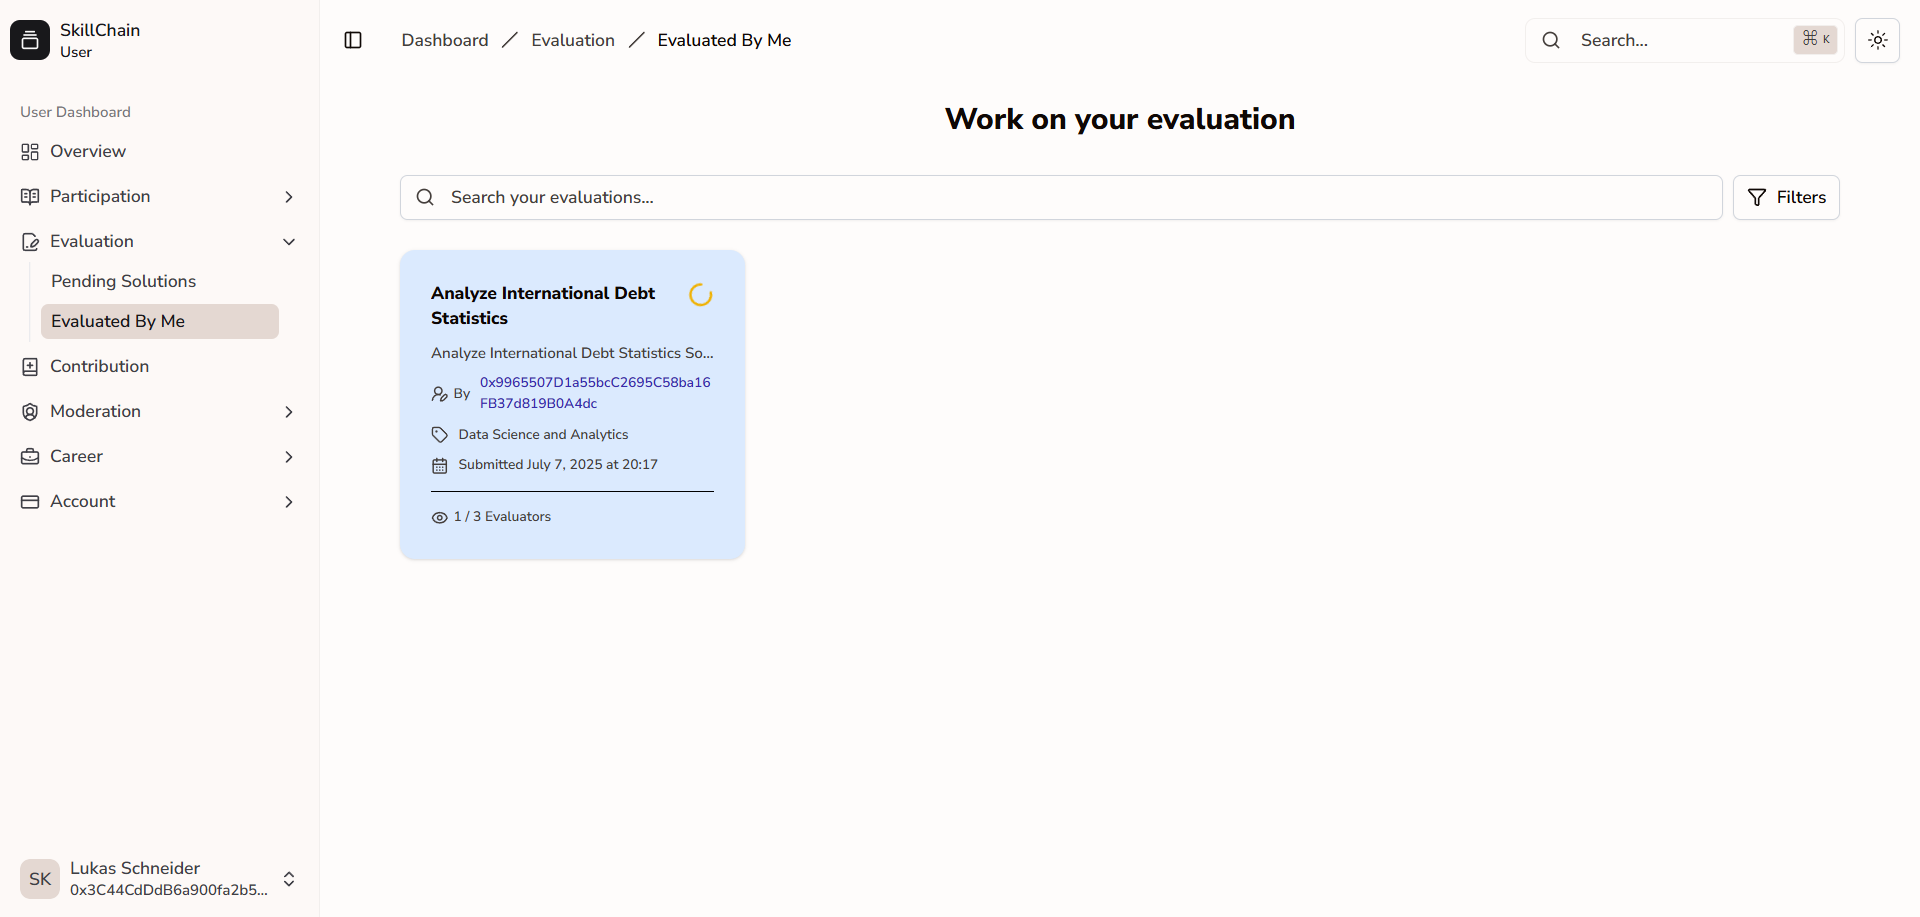
\includegraphics[width=0.99\textwidth, frame]{ui/evaluated-by-me-page.png}
  \caption{Trang danh sách giải pháp đã và đang đánh giá}
  \label{fig:evaluated-by-me-page}
\end{figure}

Người dùng thực hiện đánh giá bằng cách điền nội dung nhận xét, chấm điểm theo thang điểm quy định và nhấn ``Submit'' để nộp kết quả.  
Sau khi gửi đi, kết quả đánh giá sẽ được khóa và không thể chỉnh sửa.

\begin{figure}[H]
  \centering
  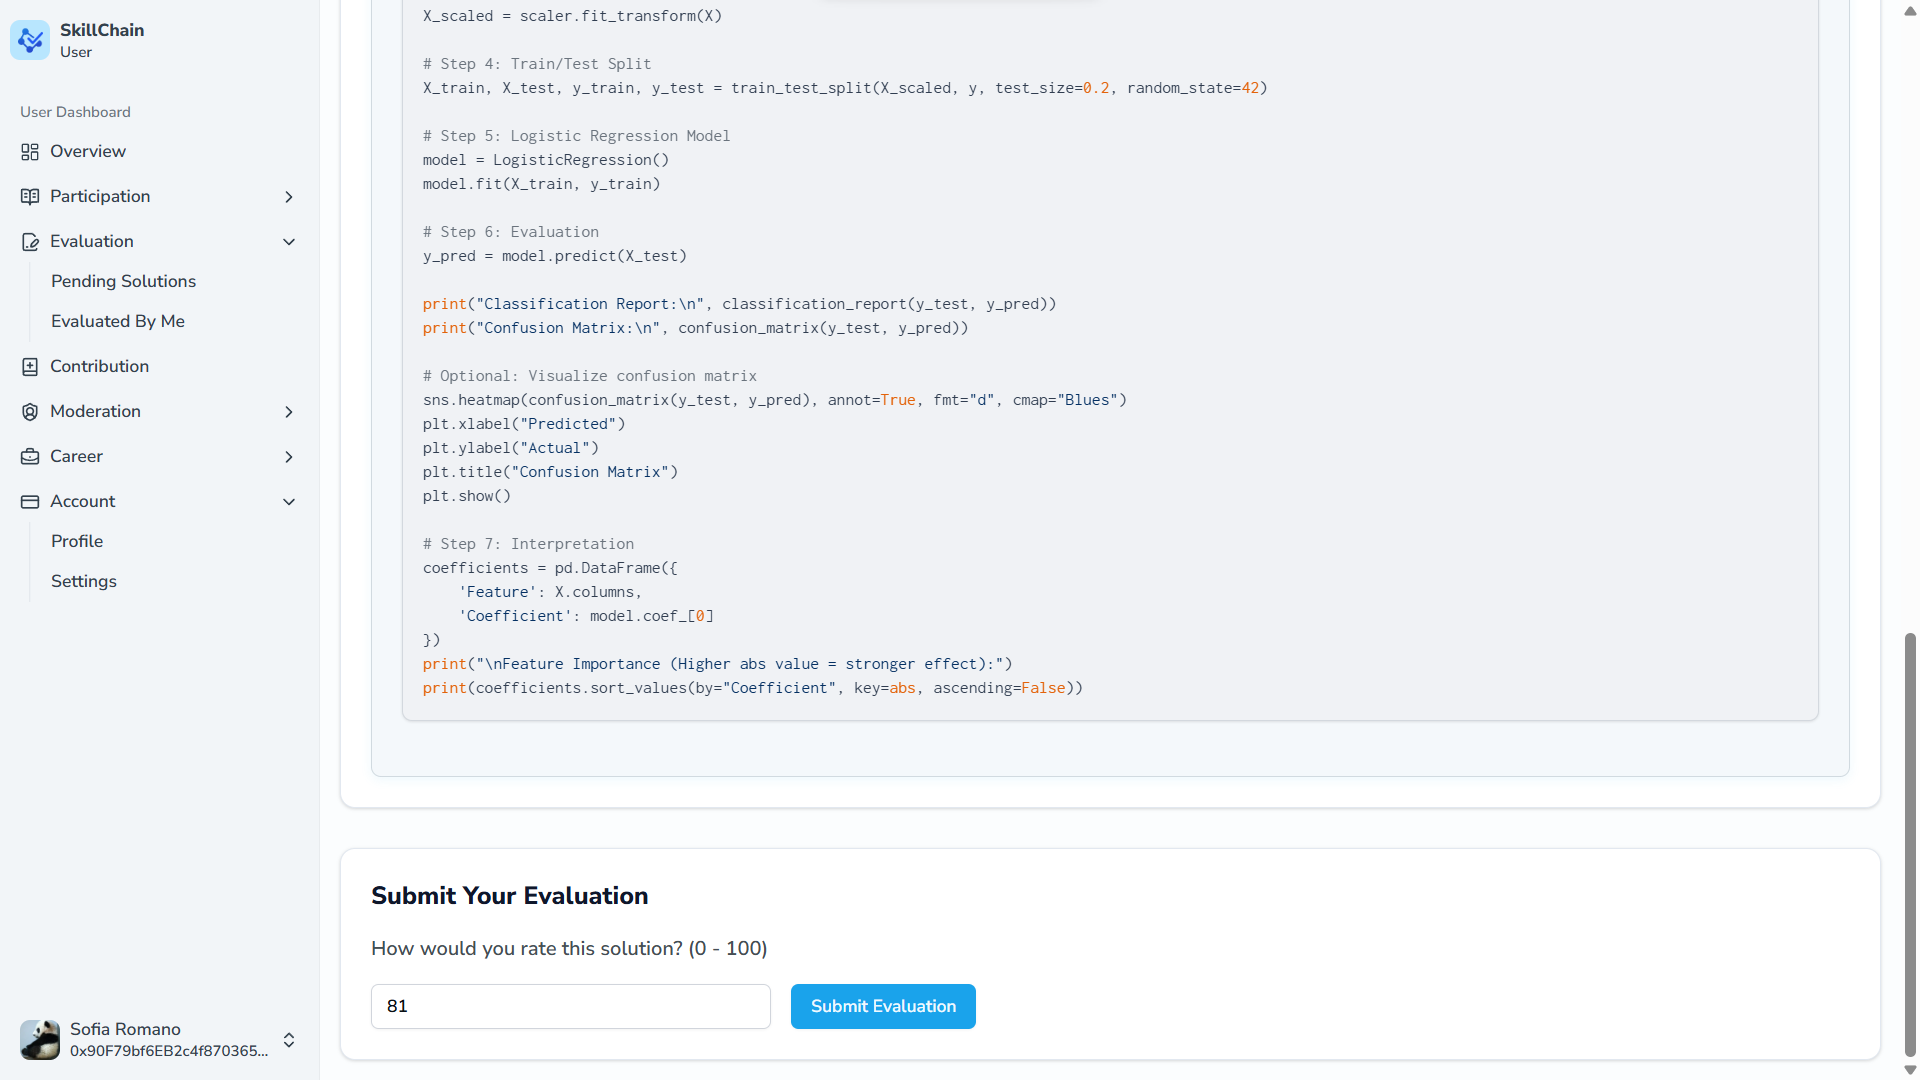
\includegraphics[width=0.99\textwidth, frame]{ui/evaluate-solution-page.png}
  \caption{Trang thực hiện đánh giá giải pháp}
  \label{fig:evaluate-solution-page}
\end{figure}

Sau khi quá trình đánh giá hoàn tất, hệ thống sẽ công khai kết quả phiên đánh giá cho cả người giải và các người đánh giá cũng như cập nhật số người hoàn thành thử thách. 

\begin{figure}[H]
  \centering
  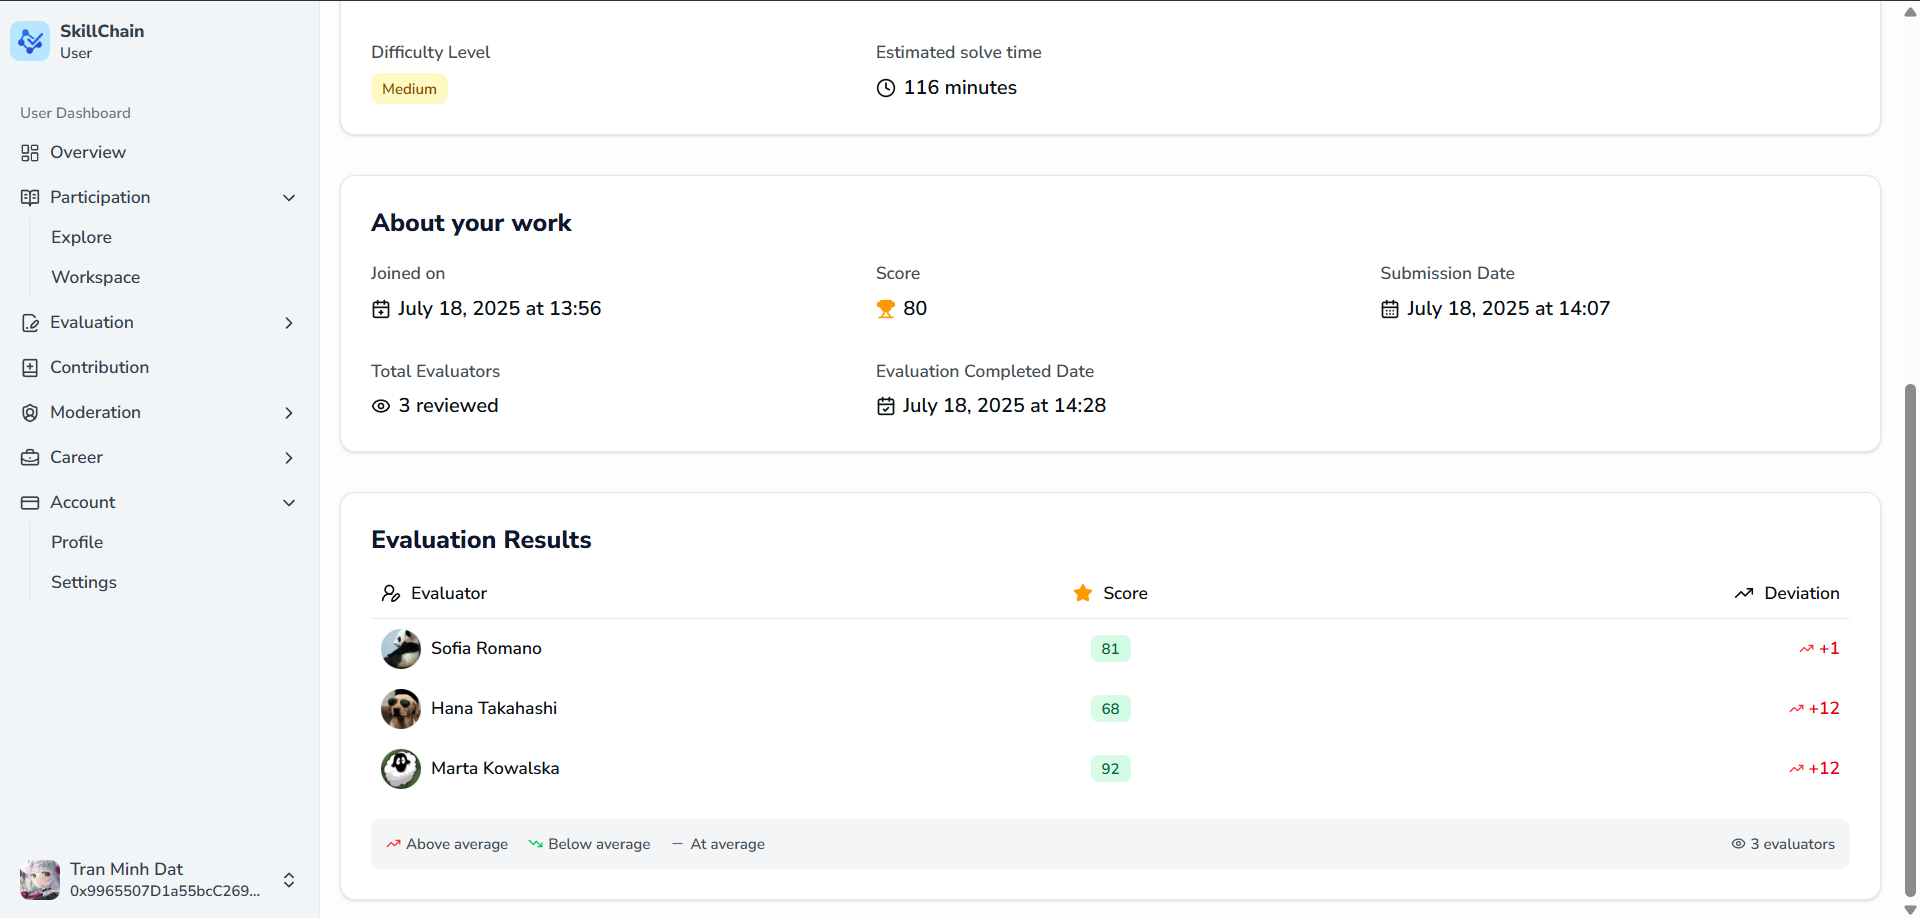
\includegraphics[width=0.99\textwidth, frame]{ui/evaluated-solution-page.png}
  \caption{Giải pháp đã được đánh giá hoàn tất}
  \label{fig:evaluated-solution-page}
\end{figure}

\section{Giao diện tuyển dụng nhân sự}

\subsection{Truy cập không gian nhà tuyển dụng}

Để chuyển sang không gian nhà tuyển dụng, người dùng kết nối ví như thông thường.  
Tại thanh thông tin cá nhân (góc trái bên dưới giao diện), nhấn vào biểu tượng tài khoản và chọn tùy chọn ``Switch to Recruiter''.  
Hệ thống sẽ tự động điều hướng sang không gian làm việc dành riêng cho nhà tuyển dụng.

\begin{figure}[H]
  \centering
  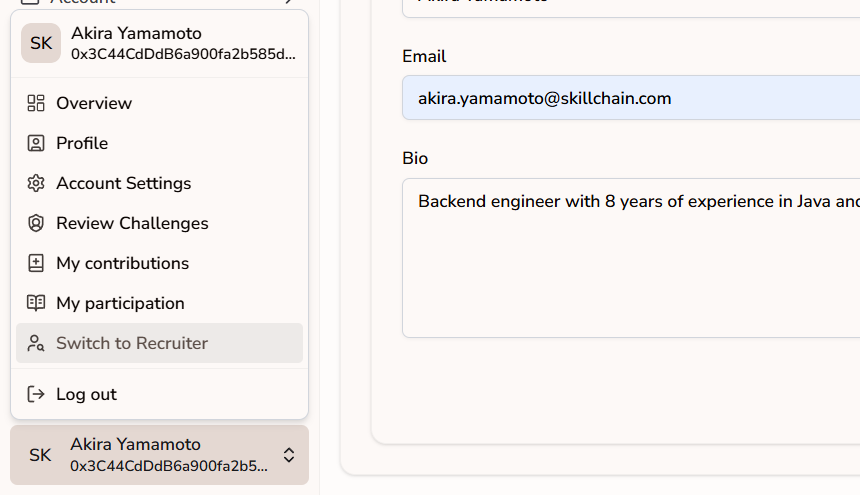
\includegraphics[width=0.99\textwidth, frame]{ui/access-recruiter-space.png}
  \caption{Truy cập không gian nhà tuyển dụng}
  \label{fig:access-recruiter-space}
\end{figure}

\subsection{Tài khoản nhà tuyển dụng}

Tại không gian nhà tuyển dụng, người dùng truy cập tab \textbf{Account} để quản lý hồ sơ cá nhân, thông tin công ty, cũng như thiết lập cấu hình liên quan đến quá trình tuyển dụng.

\subsubsection{Đăng ký trở thành nhà tuyển dụng}

Để sử dụng tính năng tuyển dụng, hệ thống yêu cầu người dùng ký gửi tối thiểu \textbf{1 ETH}.  
Để thực hiện, nhà tuyển dụng truy cập tab \textbf{Account Settings}, nhập số ETH muốn gửi tại mục ``Recruiter Budget'' và nhấn nút ``Deposit''.  
Sau đó, xác nhận giao dịch thông qua ví tiền điện tử.  
Các chi phí phát sinh trong quá trình tuyển dụng sẽ tự động được khấu trừ từ khoản ký gửi này.

\begin{figure}[H]
  \centering
  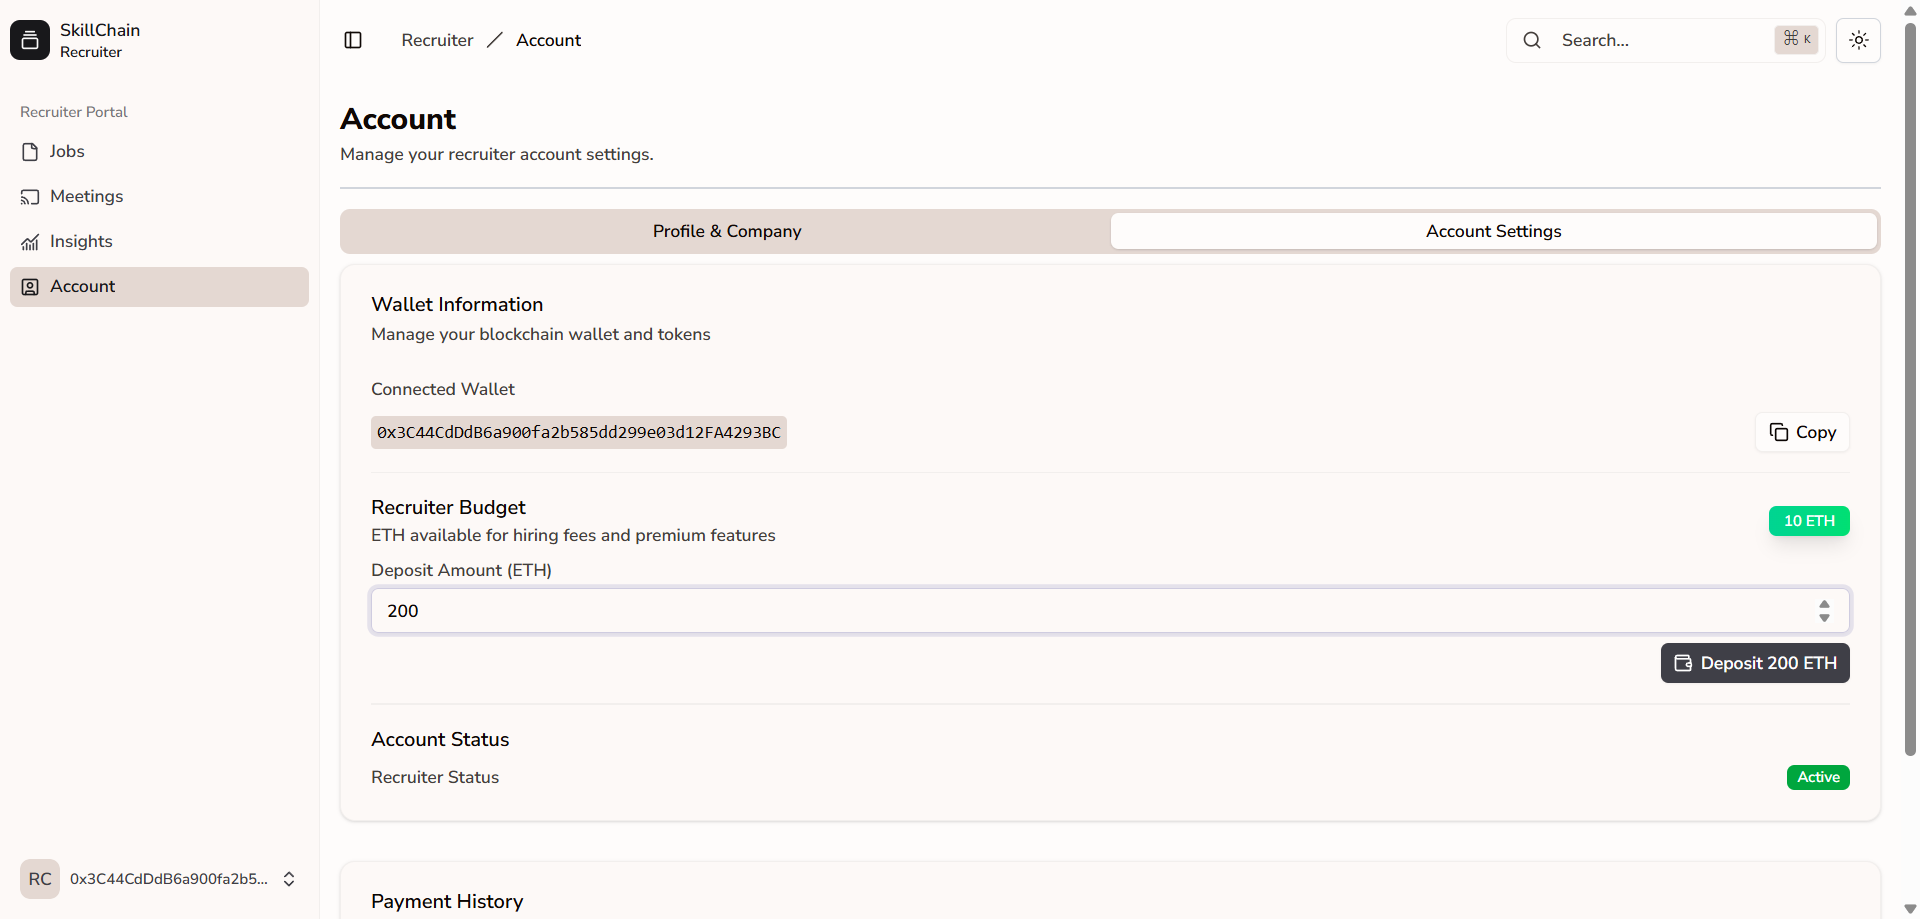
\includegraphics[width=0.99\textwidth, frame]{ui/recruiter-account-settings-page.png}
  \caption{Trang thiết lập tài khoản nhà tuyển dụng}
  \label{fig:recruiter-account-settings-page}
\end{figure}

\subsubsection{Quản lý hồ sơ nhà tuyển dụng}

Tại tab \textbf{Profile \& Company}, nhà tuyển dụng có thể đăng ký hoặc cập nhật hồ sơ cá nhân và thông tin công ty.  
Trong lần truy cập đầu tiên, hệ thống yêu cầu xác thực giao dịch qua ví điện tử để hoàn tất đăng ký.

\begin{figure}[H]
  \centering
  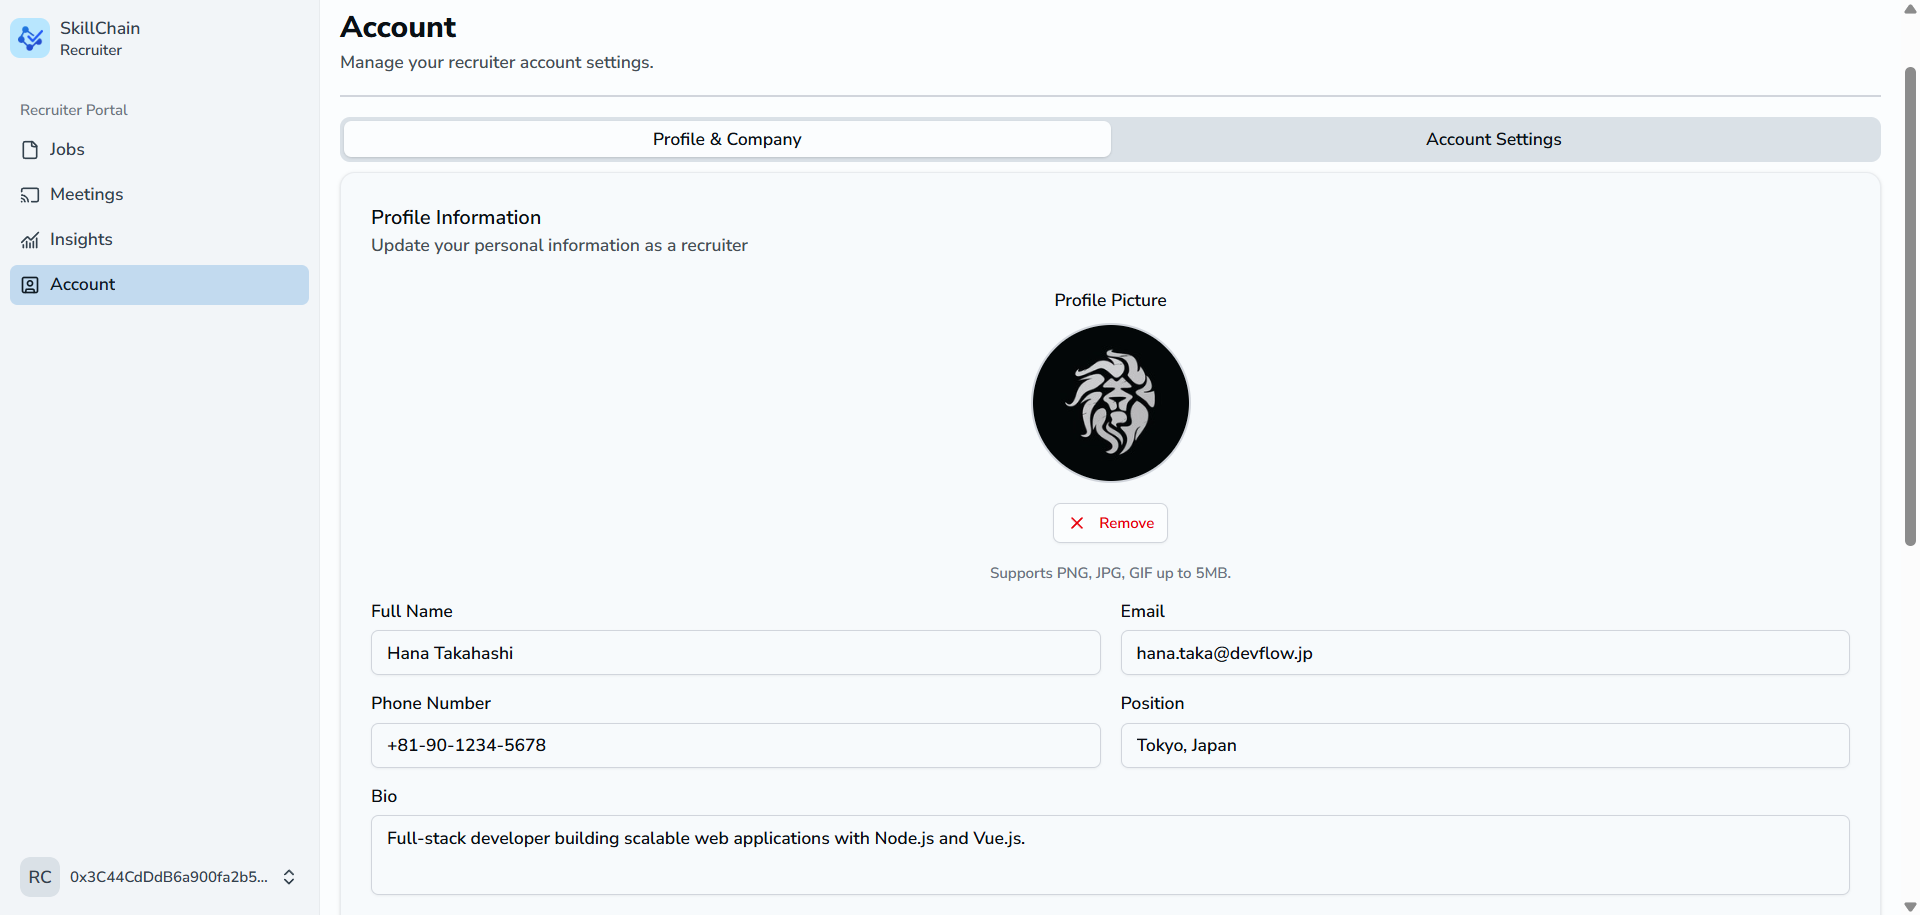
\includegraphics[width=0.99\textwidth, frame]{ui/recruiter-personal-profile.png}
  \caption{Hồ sơ cá nhân nhà tuyển dụng}
  \label{fig:recruiter-personal-profile}
\end{figure}

\begin{figure}[H]
  \centering
  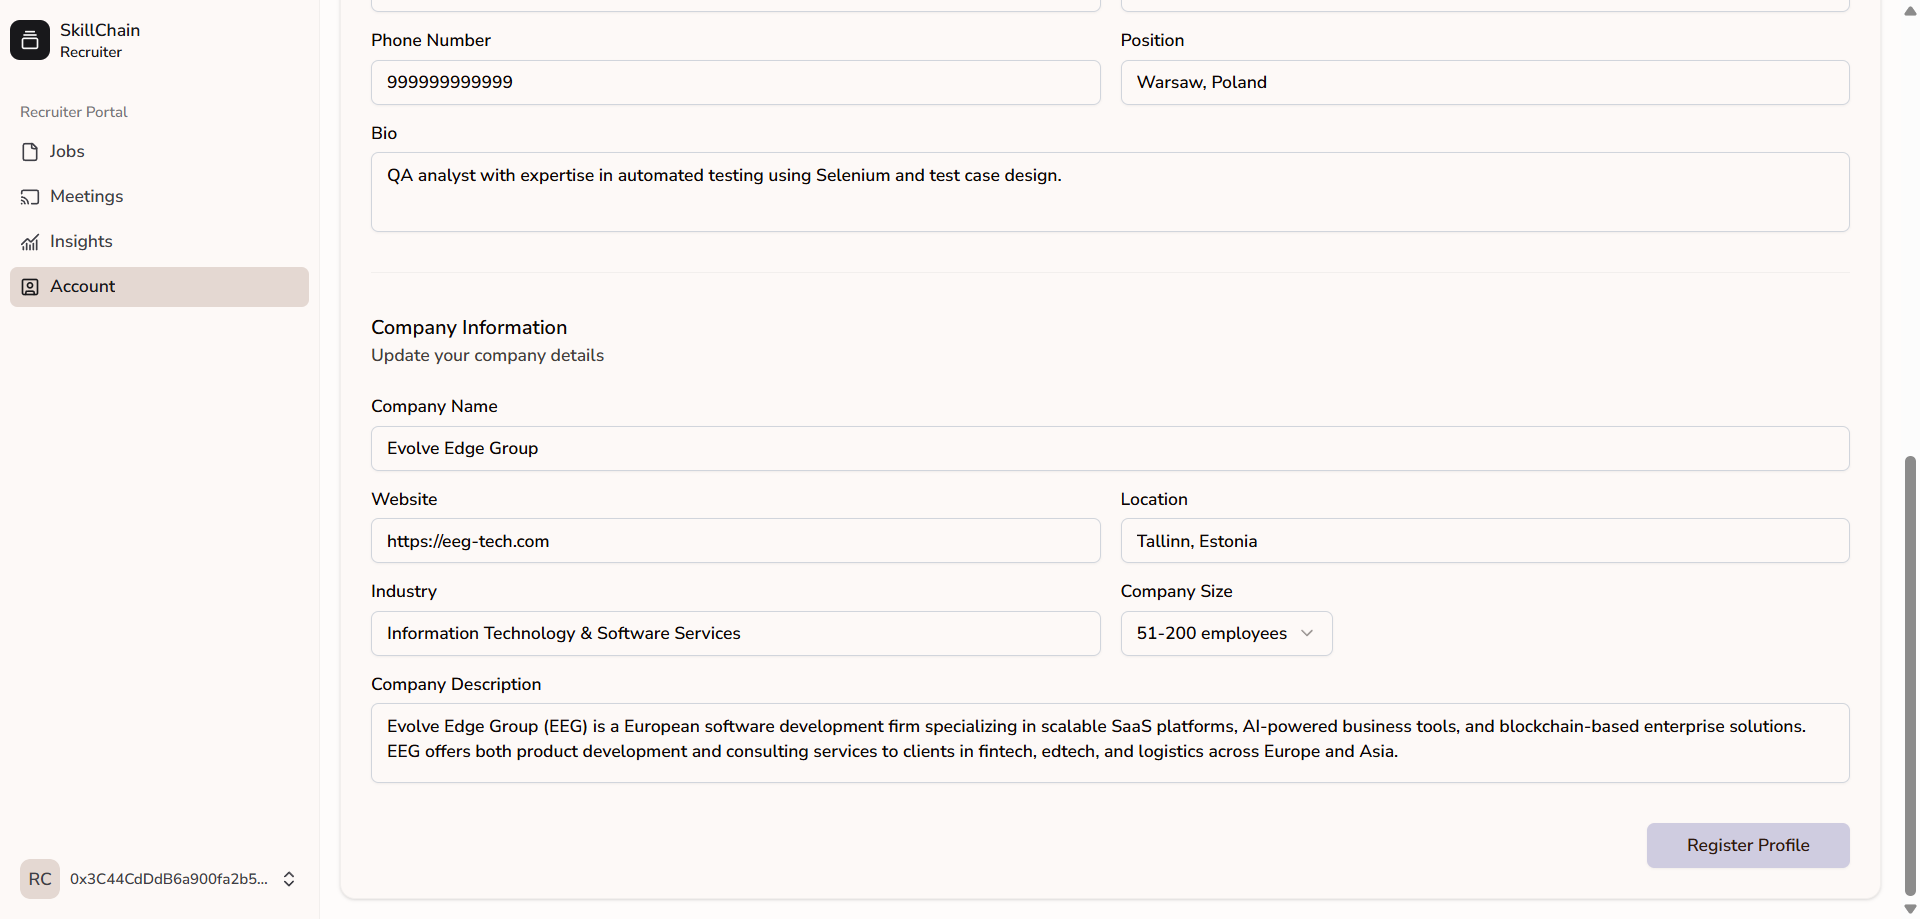
\includegraphics[width=0.99\textwidth, frame]{ui/recruiter-company-profile.png}
  \caption{Thông tin công ty của nhà tuyển dụng}
  \label{fig:recruiter-company-profile}
\end{figure}

\subsection{Quản lý bài đăng}

\subsubsection{Xem danh sách các bài đăng tuyển dụng}

Để xem danh sách các bài đăng tuyển dụng, nhà tuyển dụng truy cập tab \textbf{Jobs}.  
Tại đây, hệ thống hiển thị danh sách các bài đăng đã tạo cùng với thông tin trạng thái, số lượng ứng viên đã ứng tuyển và các hành động có thể thực hiện.

\begin{figure}[H]
  \centering
  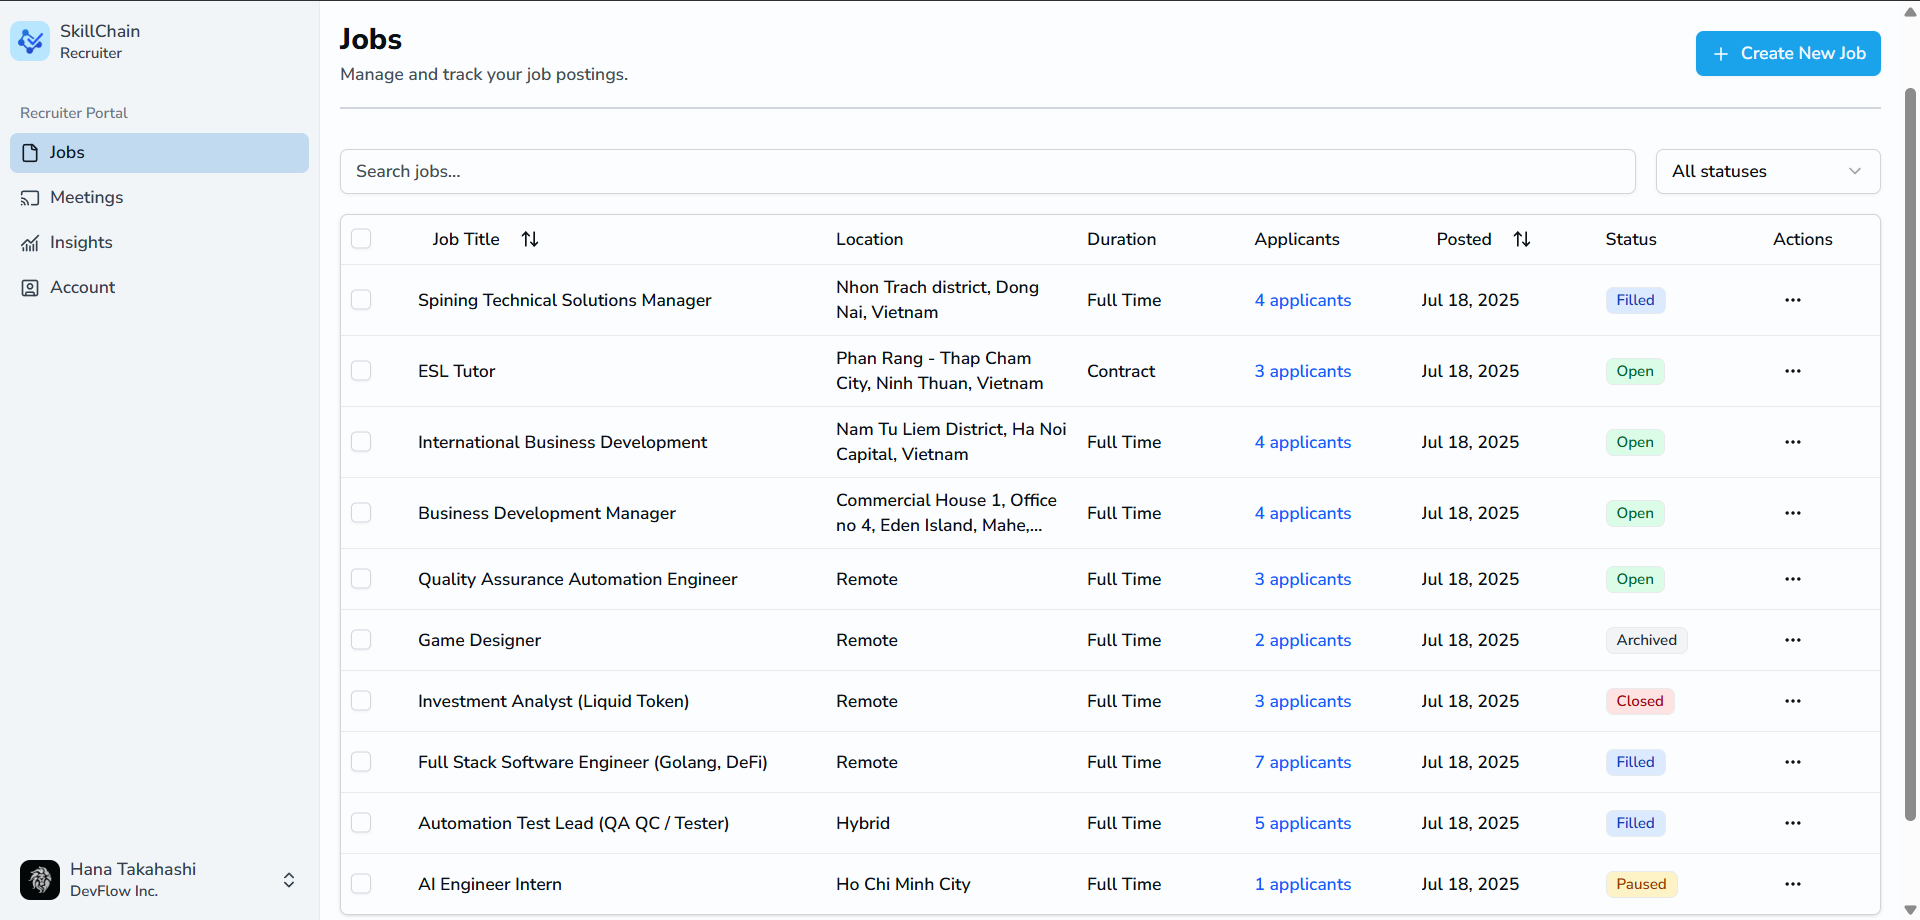
\includegraphics[width=0.99\textwidth, frame]{ui/jobs-page.png}
  \caption{Trang danh sách các bài đăng tuyển dụng}
  \label{fig:jobs-page}
\end{figure}

Để xem chi tiết một bài đăng, nhà tuyển dụng nhấn ``View job'' tại nút ``Actions'' tương ứng.

\begin{figure}[H]
  \centering
  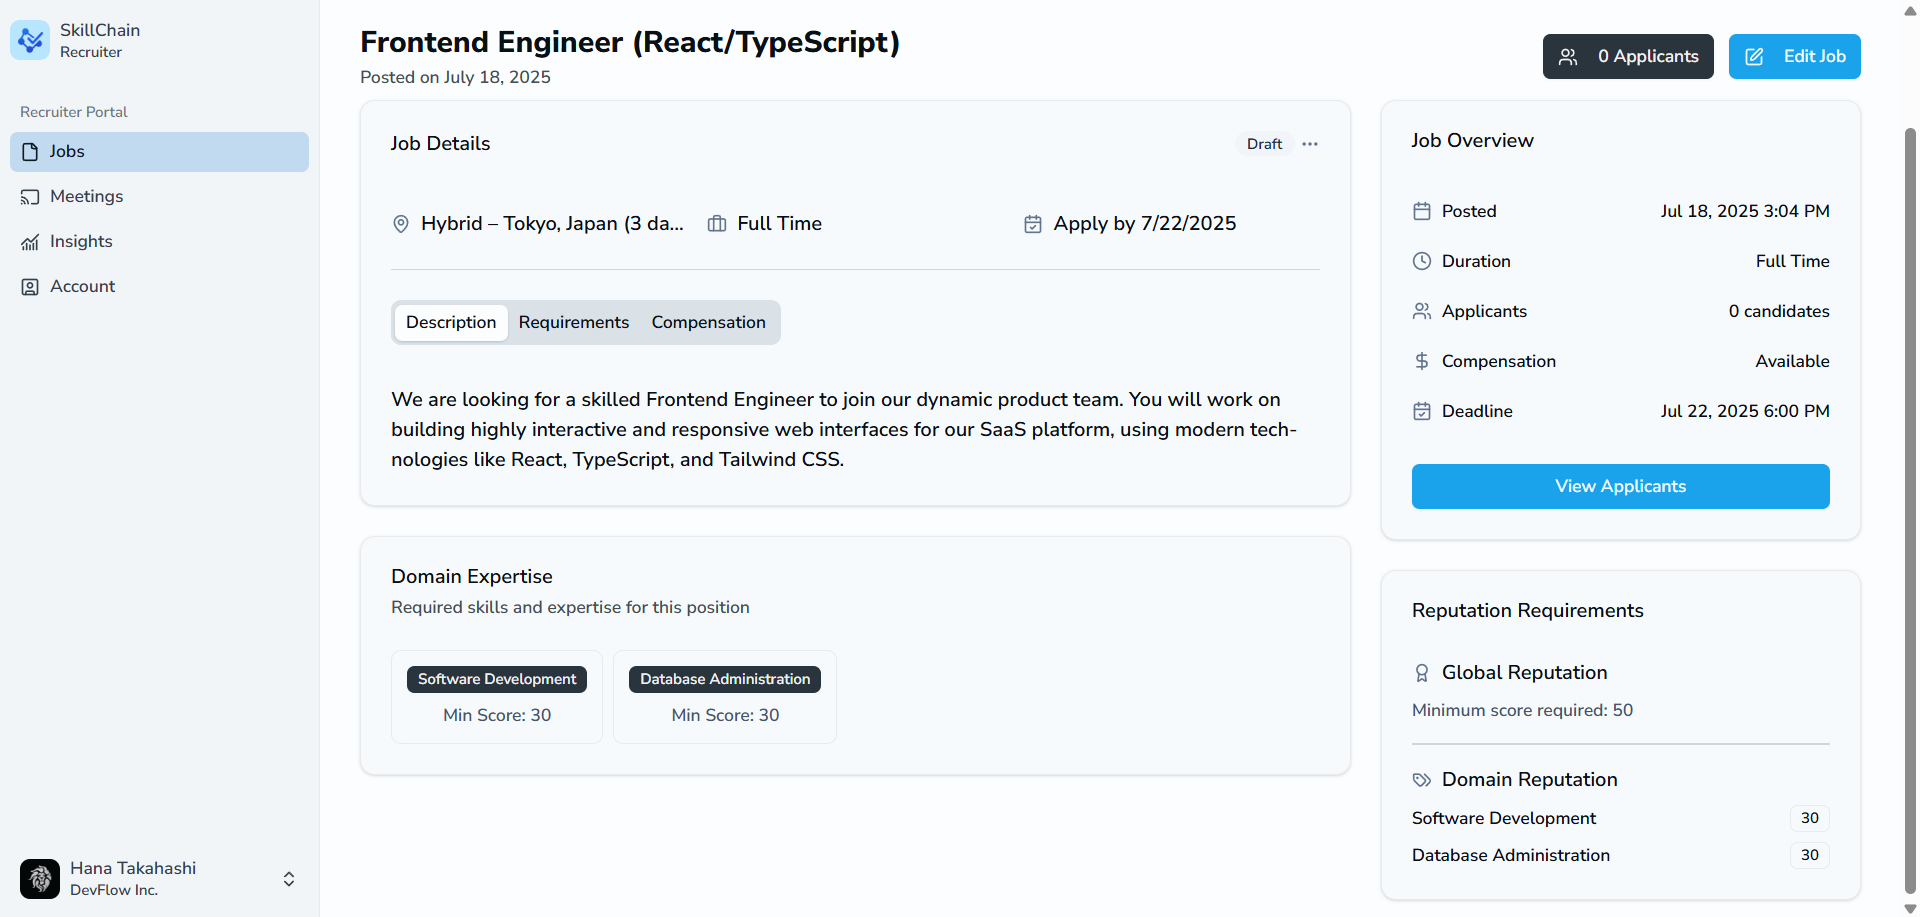
\includegraphics[width=0.99\textwidth, frame]{ui/job-detail-page.png}
  \caption{Trang chi tiết một bài đăng tuyển dụng}
  \label{fig:job-detail-page}
\end{figure}

\subsubsection{Tạo bài đăng tuyển dụng mới}

Để tạo bài đăng mới, nhà tuyển dụng nhấn nút ``Create New Job'' ở góc trên bên phải.  
Tại giao diện tạo bài đăng, nhà tuyển dụng nhập thông tin vị trí công việc, thời hạn đăng bài, cùng với các yêu cầu về uy tín đối với ứng viên.  
Sau khi hoàn tất, nhấn nút ``Create Job'' và xác nhận giao dịch qua ví điện tử để tạo bài đăng ở trạng thái nháp.

\begin{figure}[H]
  \centering
  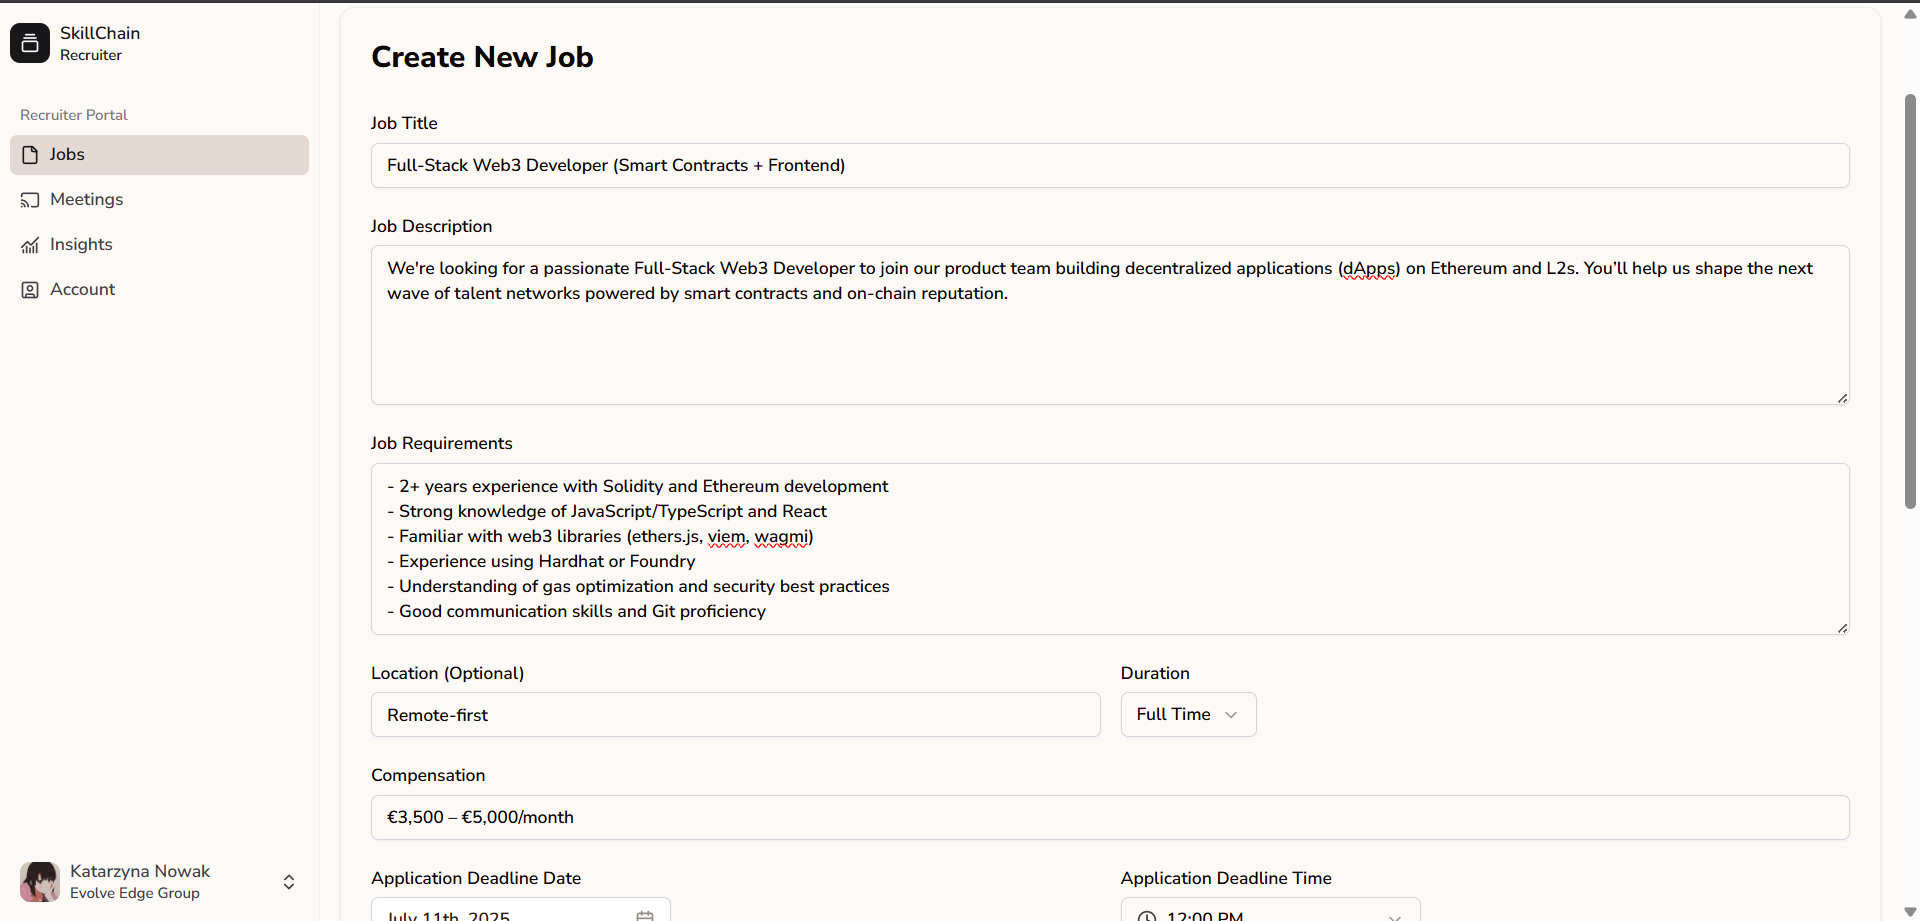
\includegraphics[width=0.99\textwidth, frame]{ui/job-position-info.png}
  \caption{Thông tin về vị trí công việc}
  \label{fig:job-position-info}
\end{figure}

\begin{figure}[H]
  \centering
  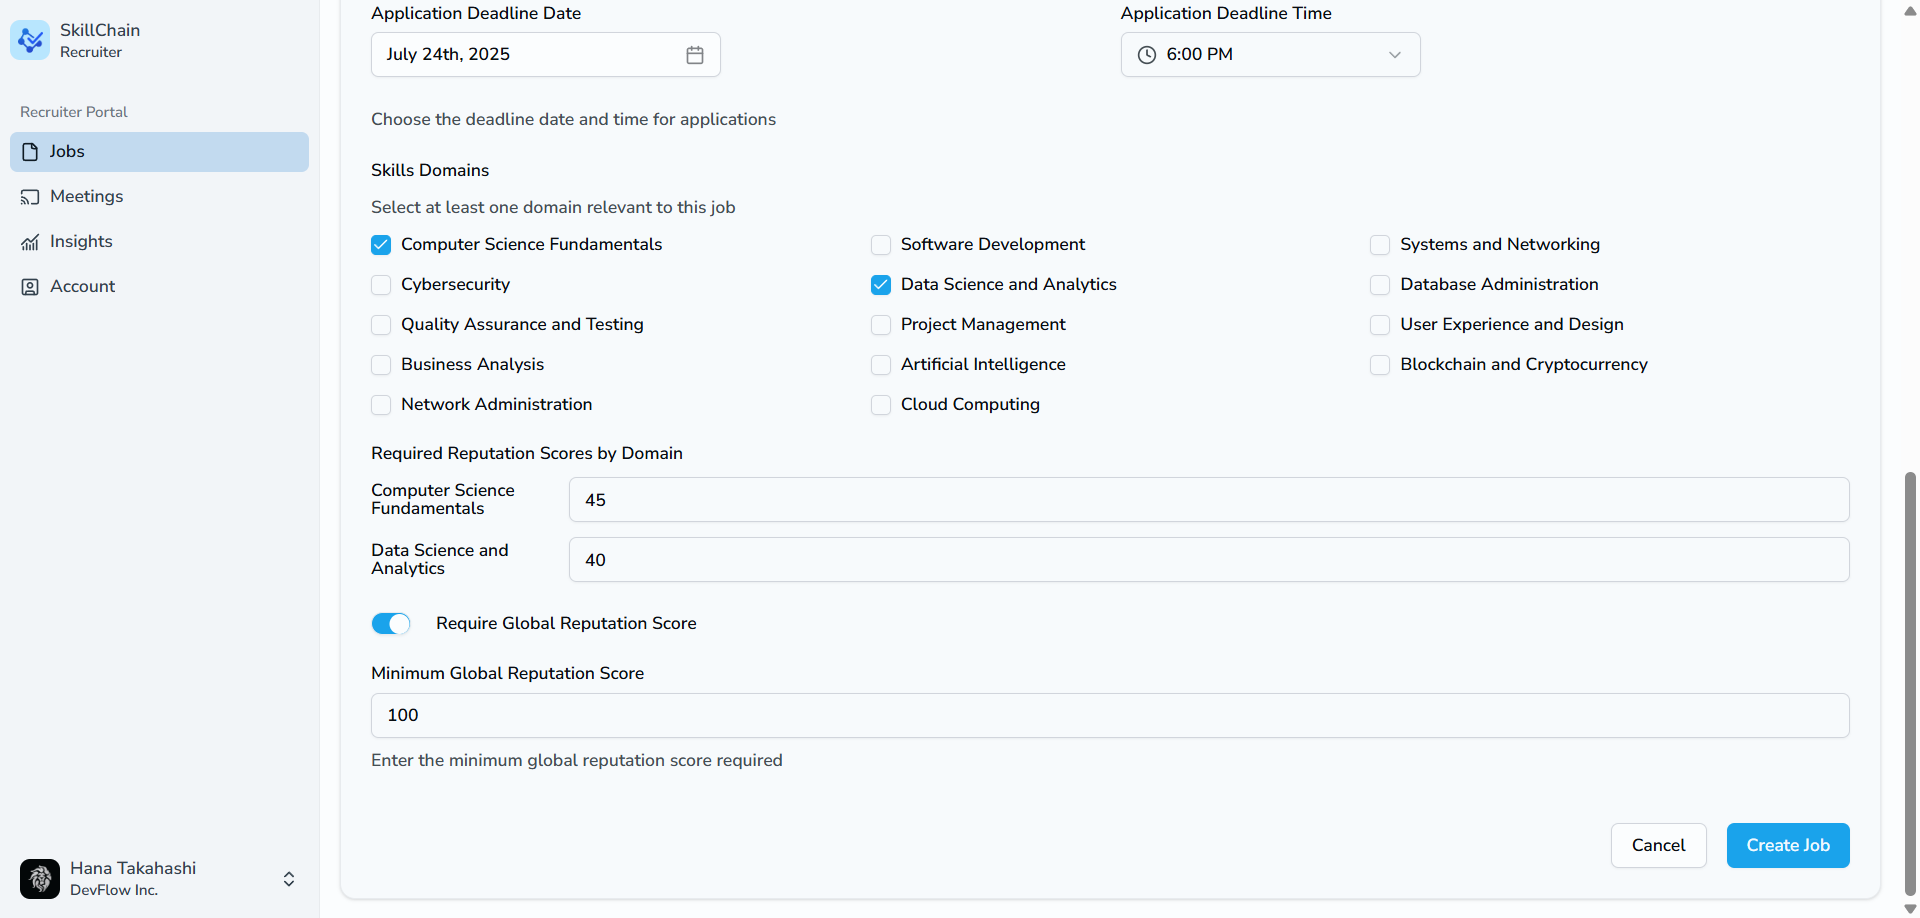
\includegraphics[width=0.99\textwidth, frame]{ui/job-reputation-requirement.png}
  \caption{Yêu cầu uy tín đối với ứng viên}
  \label{fig:job-reputation-requirement}
\end{figure}

\subsubsection{Chỉnh sửa nội dung bài đăng}

Để chỉnh sửa nội dung bài đăng, nhà tuyển dụng có thể thực hiện theo hai cách:
\begin{itemize}
  \item Từ trang chi tiết bài đăng, nhấn ``Edit Job'' ở góc trên bên phải.
  \item Từ danh sách bài đăng, chọn ``Edit job'' tại mục ``Actions''.
\end{itemize}

Hệ thống cho phép chỉnh sửa nội dung trong mọi trạng thái bài đăng mà không phát sinh giao dịch.

\begin{figure}[H]
  \centering
  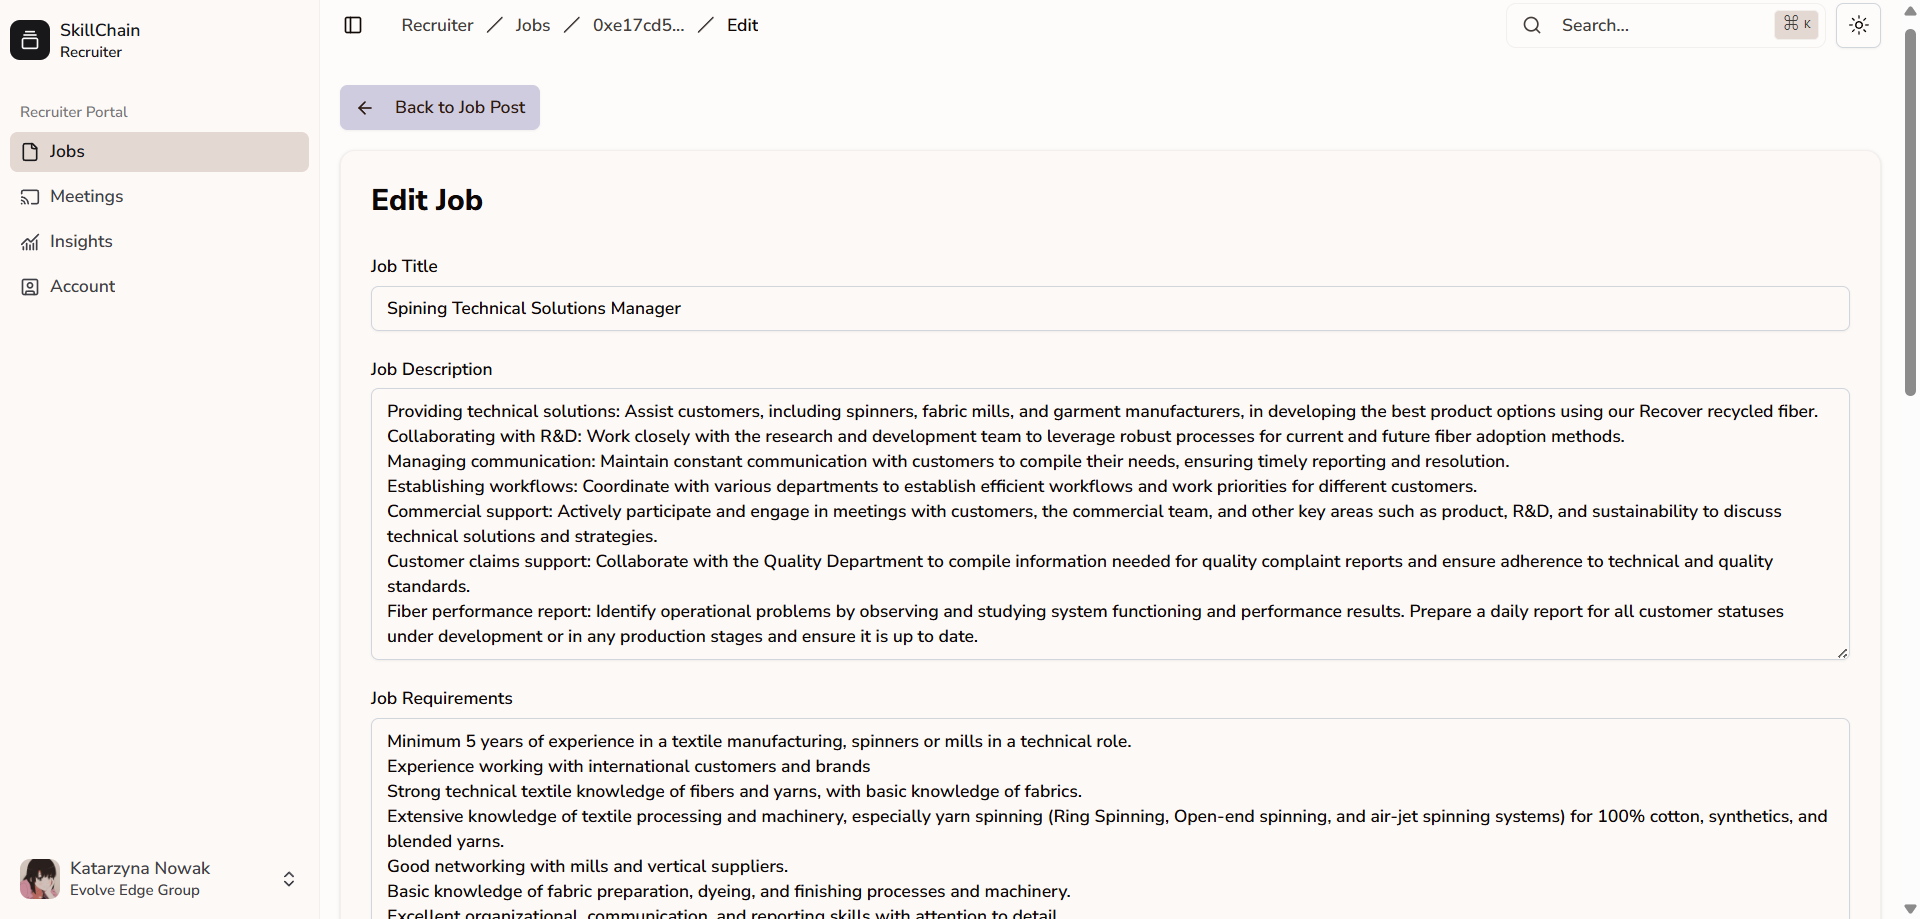
\includegraphics[width=0.99\textwidth, frame]{ui/edit-job-page.png}
  \caption{Trang chỉnh sửa bài đăng tuyển dụng}
  \label{fig:edit-job-page}
\end{figure}

\subsubsection{Chuyển đổi trạng thái bài đăng}

Tại trang chi tiết bài đăng, để thay đổi trạng thái (ví dụ: từ ``nháp'' sang ``đang mở''), nhà tuyển dụng nhấn biểu tượng ba chấm bên cạnh thông tin trạng thái trong phần ``Job Details'' và chọn trạng thái mong muốn.  
Thao tác này yêu cầu xác nhận giao dịch qua ví điện tử.

\subsection{Quản lý thông tin ứng tuyển}

\subsubsection{Xem thông tin ứng tuyển}

Để xem danh sách ứng viên đã ứng tuyển cho một bài đăng, nhà tuyển dụng có thể thực hiện theo hai cách:
\begin{itemize}
  \item Từ trang chi tiết bài đăng, nhấn nút ``View Applicants'' trong phần ``Job Overview''.
  \item Từ danh sách bài đăng, chọn ``View applicants'' tại mục ``Actions'' hoặc nhấn vào liên kết tại cột ``Applicants''.
\end{itemize}

\begin{figure}[H]
  \centering
  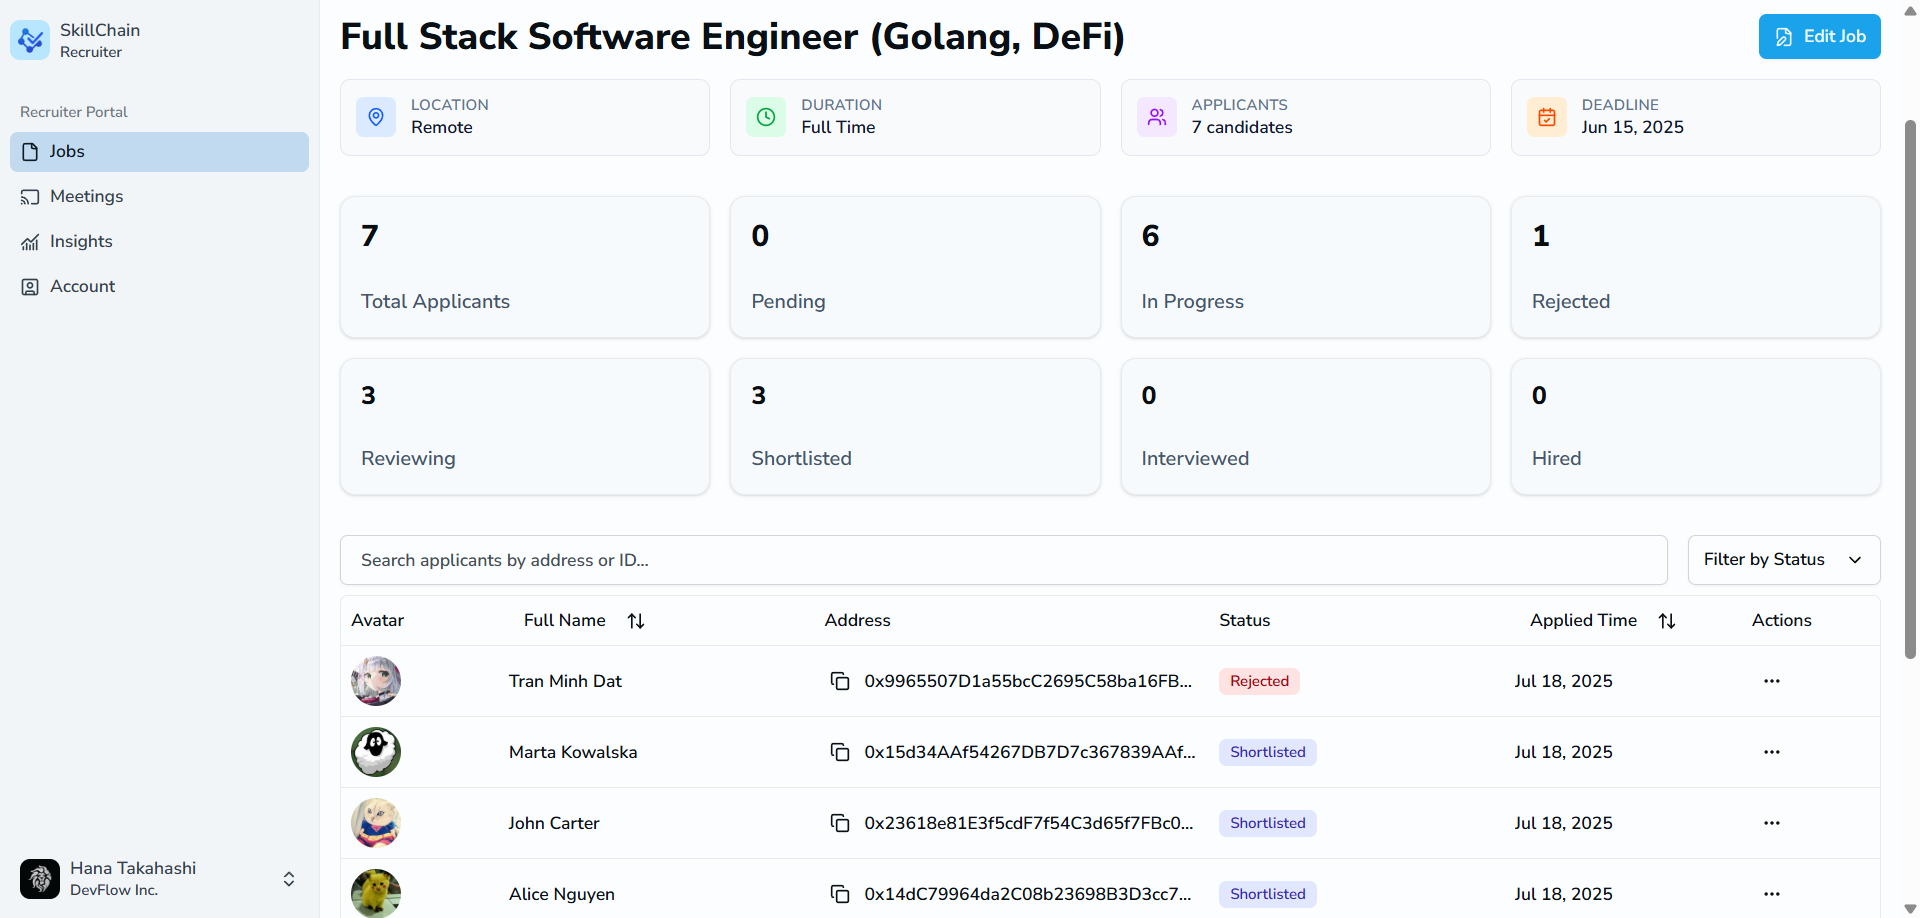
\includegraphics[width=0.99\textwidth, frame]{ui/job-applicants-list-page.png}
  \caption{Danh sách ứng viên ứng tuyển cho một bài đăng}
  \label{fig:job-applicants-list-page}
\end{figure}

Để xem chi tiết hồ sơ một ứng viên, nhà tuyển dụng nhấn ``View application'' tại mục ``Actions'' tương ứng trong danh sách.

\begin{figure}[H]
  \centering
  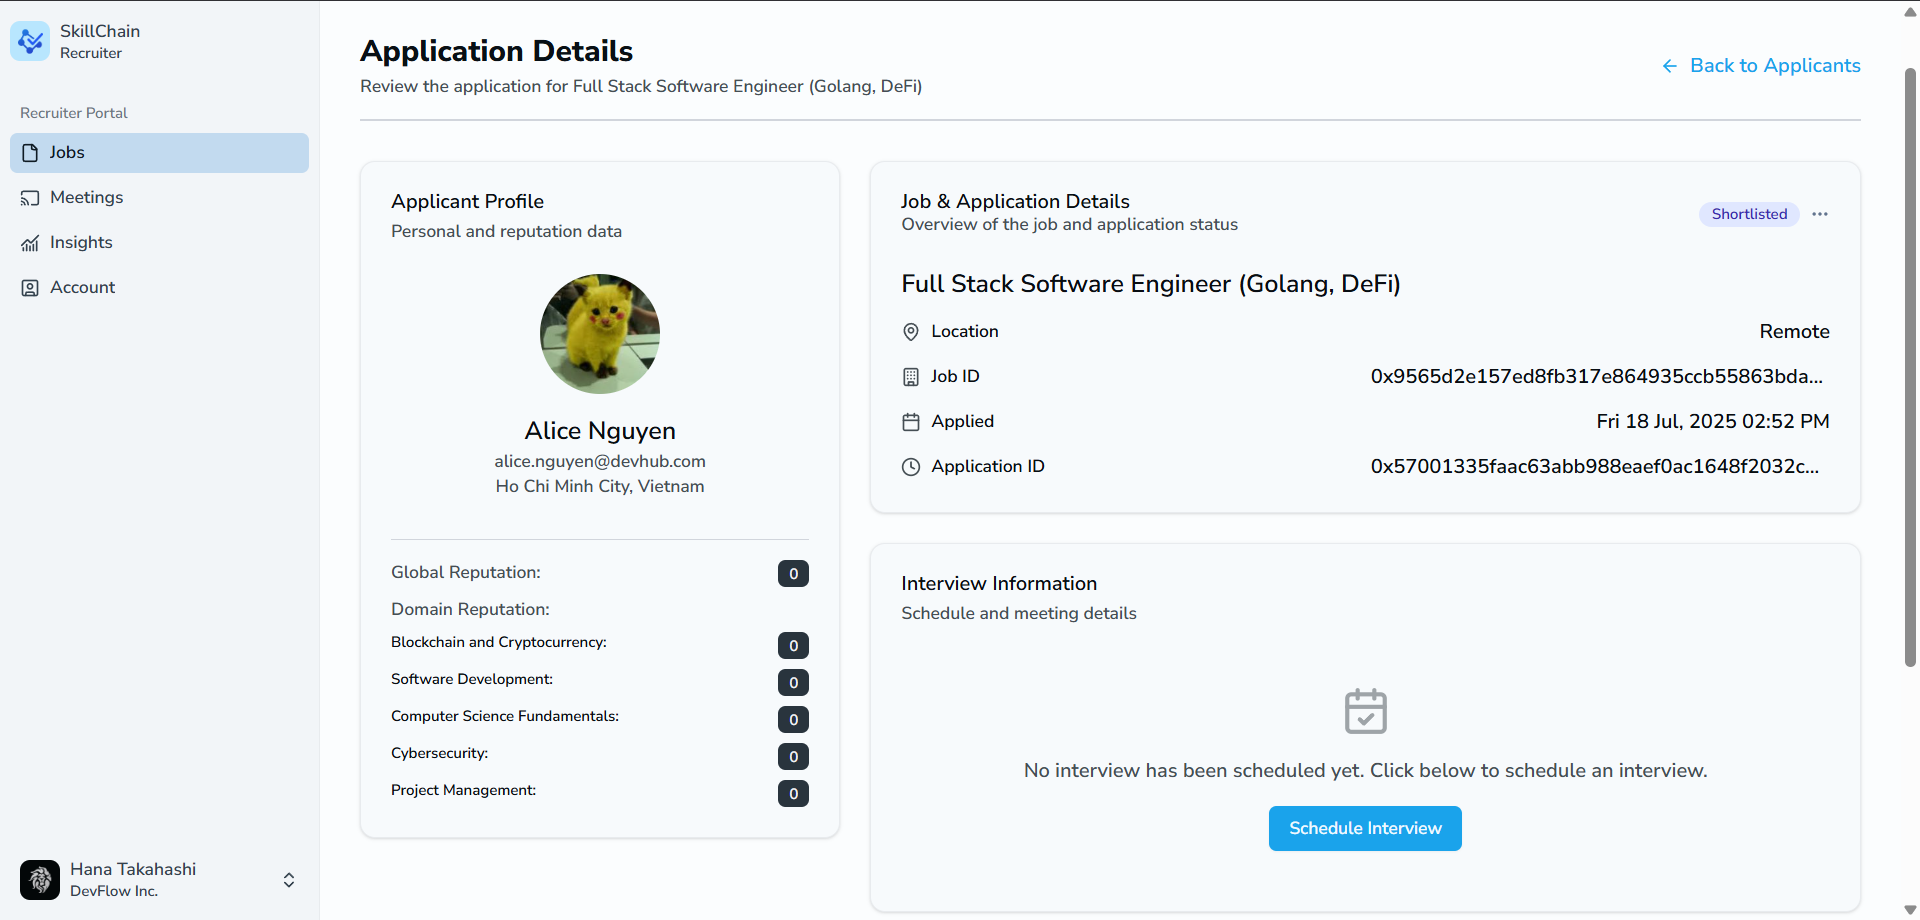
\includegraphics[width=0.99\textwidth, frame]{ui/job-applicant-detail-page.png}
  \caption{Trang chi tiết hồ sơ ứng viên}
  \label{fig:job-applicant-detail-page}
\end{figure}

\subsubsection{Chuyển đổi trạng thái ứng viên}

Tại trang chi tiết hồ sơ ứng viên, để thay đổi trạng thái (ví dụ: từ ``đã đánh giá'' sang ``được rút gọn''), nhà tuyển dụng nhấn biểu tượng ba chấm kế bên thông tin trạng thái trong phần ``Job \& Application Details'' và chọn trạng thái mong muốn.
Hành vi này cần được xác nhận giao dịch thông qua ví tiền điện tử.

\subsection{Quản lý lịch họp trực tuyến}

\subsubsection{Xem danh sách cuộc họp}

Để xem danh sách các cuộc họp đã được lên lịch, nhà tuyển dụng truy cập tab \textbf{Meetings}.  
Tại đây, hệ thống hiển thị danh sách các cuộc họp trực tuyến cùng với các thông tin như trạng thái, vị trí công việc, ứng viên liên quan và thời gian diễn ra.

\begin{figure}[H]
  \centering
  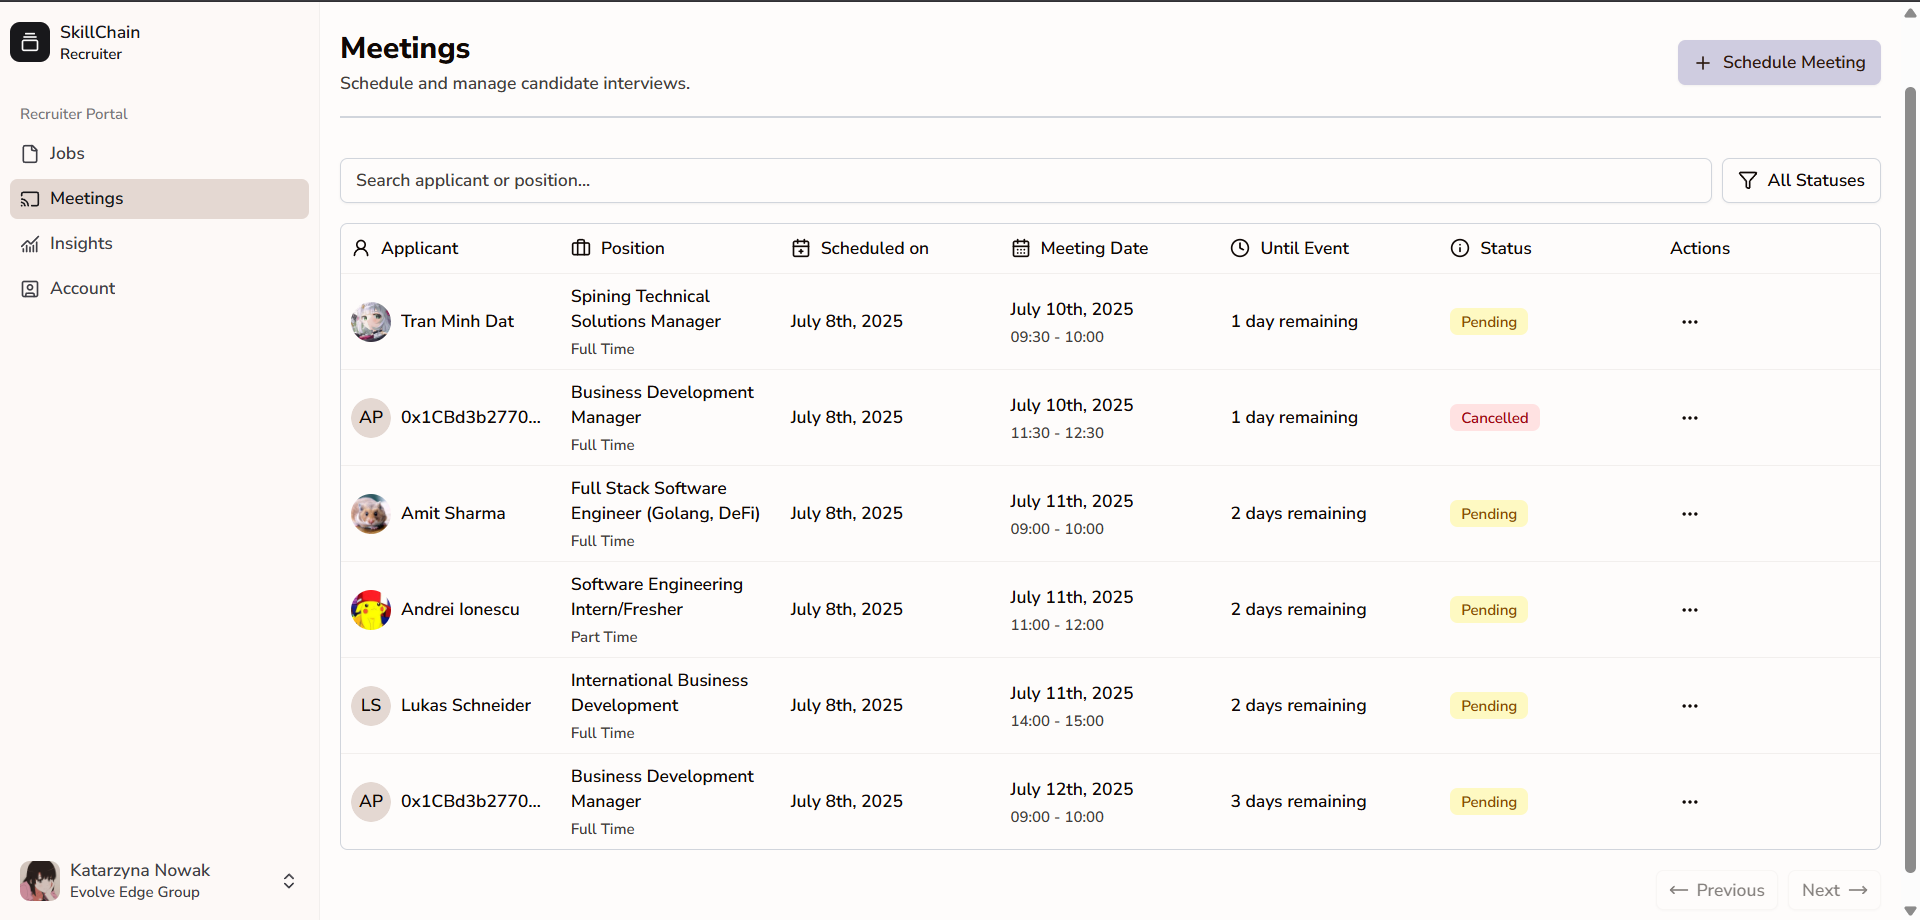
\includegraphics[width=0.99\textwidth, frame]{ui/meeting-list-page.png}
  \caption{Trang danh sách các cuộc họp trực tuyến}
  \label{fig:meeting-list-page}
\end{figure}

Để xem chi tiết một cuộc họp, nhà tuyển dụng nhấn ``View meeting'' tại mục ``Actions'' tương ứng.

\begin{figure}[H]
  \centering
  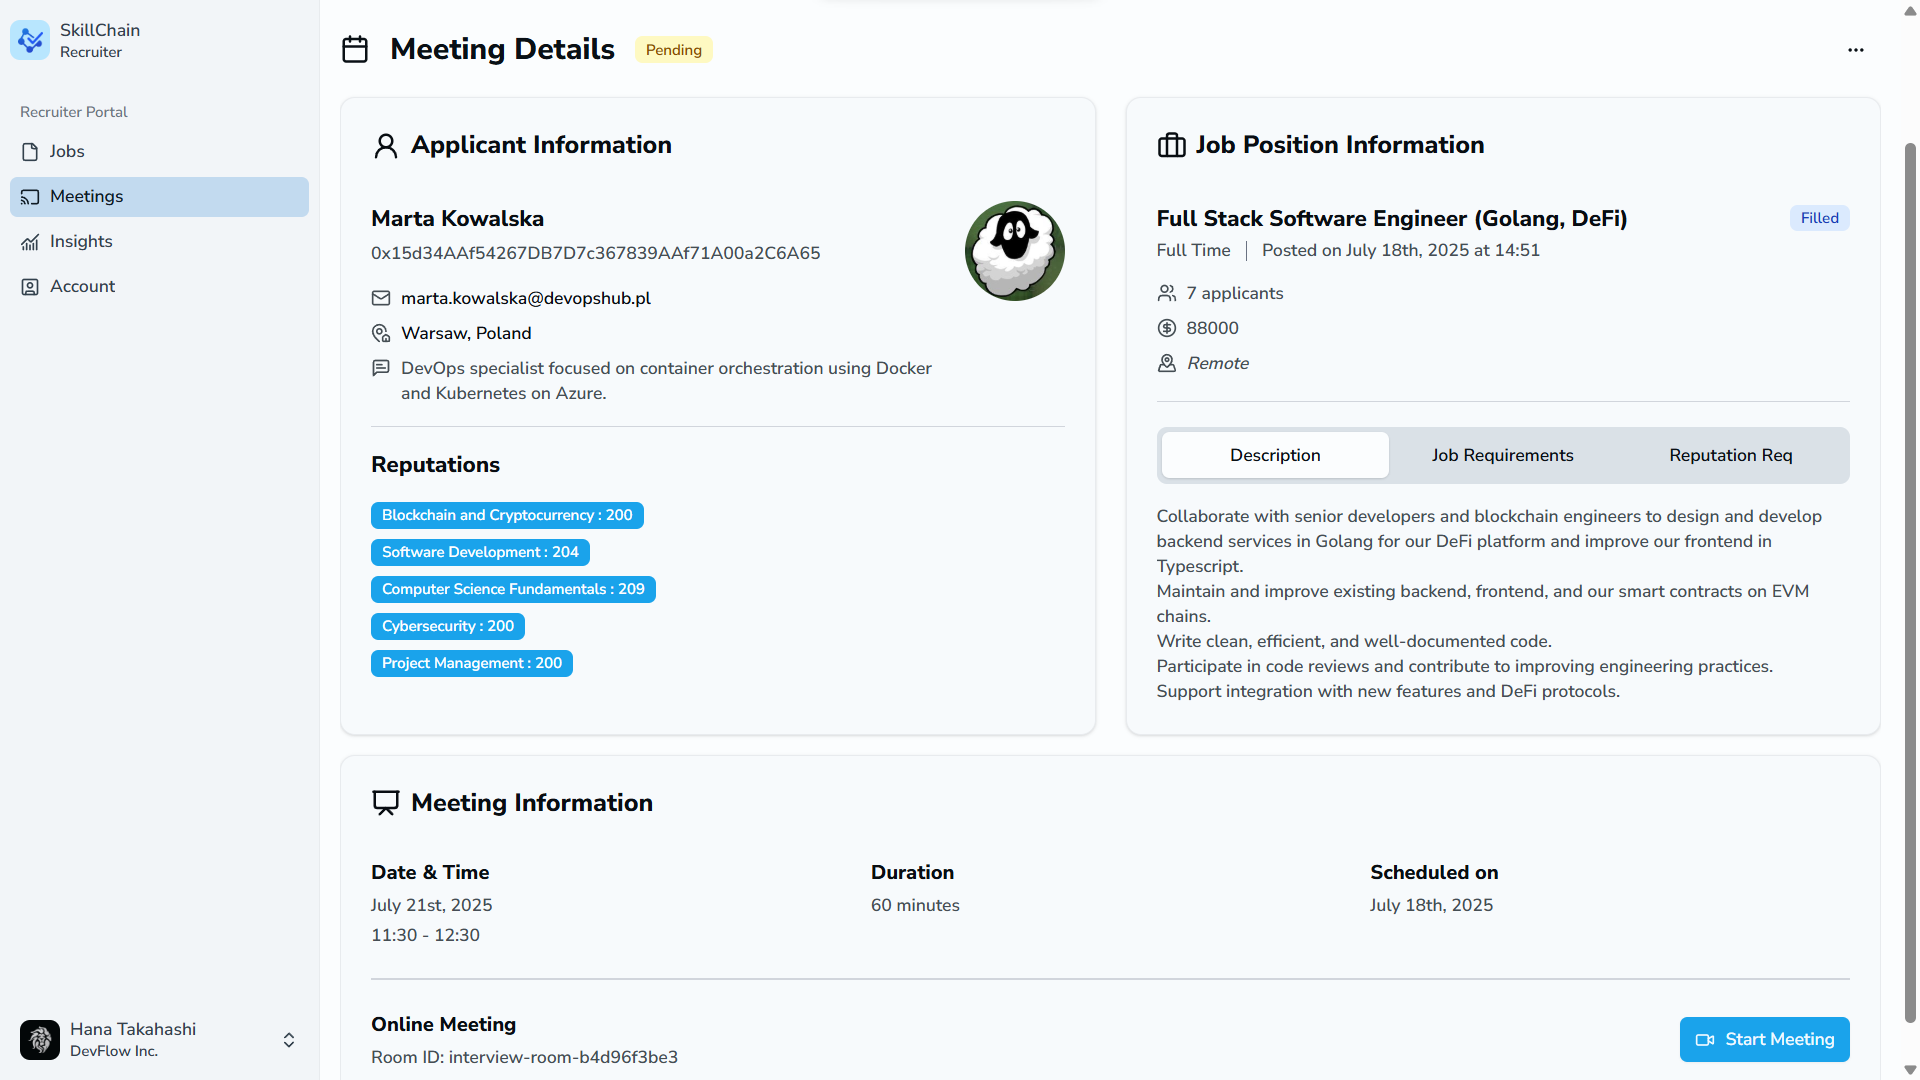
\includegraphics[width=0.99\textwidth, frame]{ui/meeting-detail-page.png}
  \caption{Trang chi tiết một cuộc họp trực tuyến}
  \label{fig:meeting-detail-page}
\end{figure}

Tại trang chi tiết cuộc họp, nhà tuyển dụng có thể đánh dấu trạng thái cuộc họp là \textit{Completed} (Đã hoàn thành) hoặc \textit{Cancelled} (Đã huỷ) bằng cách chọn biểu tượng ba chấm ở góc trên bên phải và thực hiện lựa chọn tương ứng.  
Hành động này yêu cầu xác nhận giao dịch qua ví điện tử.

\subsubsection{Lên lịch một cuộc họp mới}

Để lên lịch một cuộc họp mới, nhà tuyển dụng nhấn nút ``Schedule Meeting'' ở góc trên bên phải trang danh sách cuộc họp.

Tại biểu mẫu lên lịch, nhà tuyển dụng thực hiện các bước:
\begin{enumerate}
  \item Chọn vị trí công việc tương ứng.
  \item Chọn ứng viên thuộc \textbf{danh sách rút gọn} của vị trí đó.
  \item Chọn thời gian diễn ra cuộc họp.
  \item (Tuỳ chọn) Ghi chú gửi đến ứng viên.
\end{enumerate}

Sau khi hoàn tất, nhấn nút ``Schedule'' và xác nhận giao dịch qua ví điện tử để hoàn tất việc lên lịch.

\textbf{Lưu ý:} Nhà tuyển dụng không thể lên lịch một cuộc họp mới cho cùng một ứng viên nếu đã có cuộc họp đang chờ với ứng viên đó.

\begin{figure}[H]
  \centering
  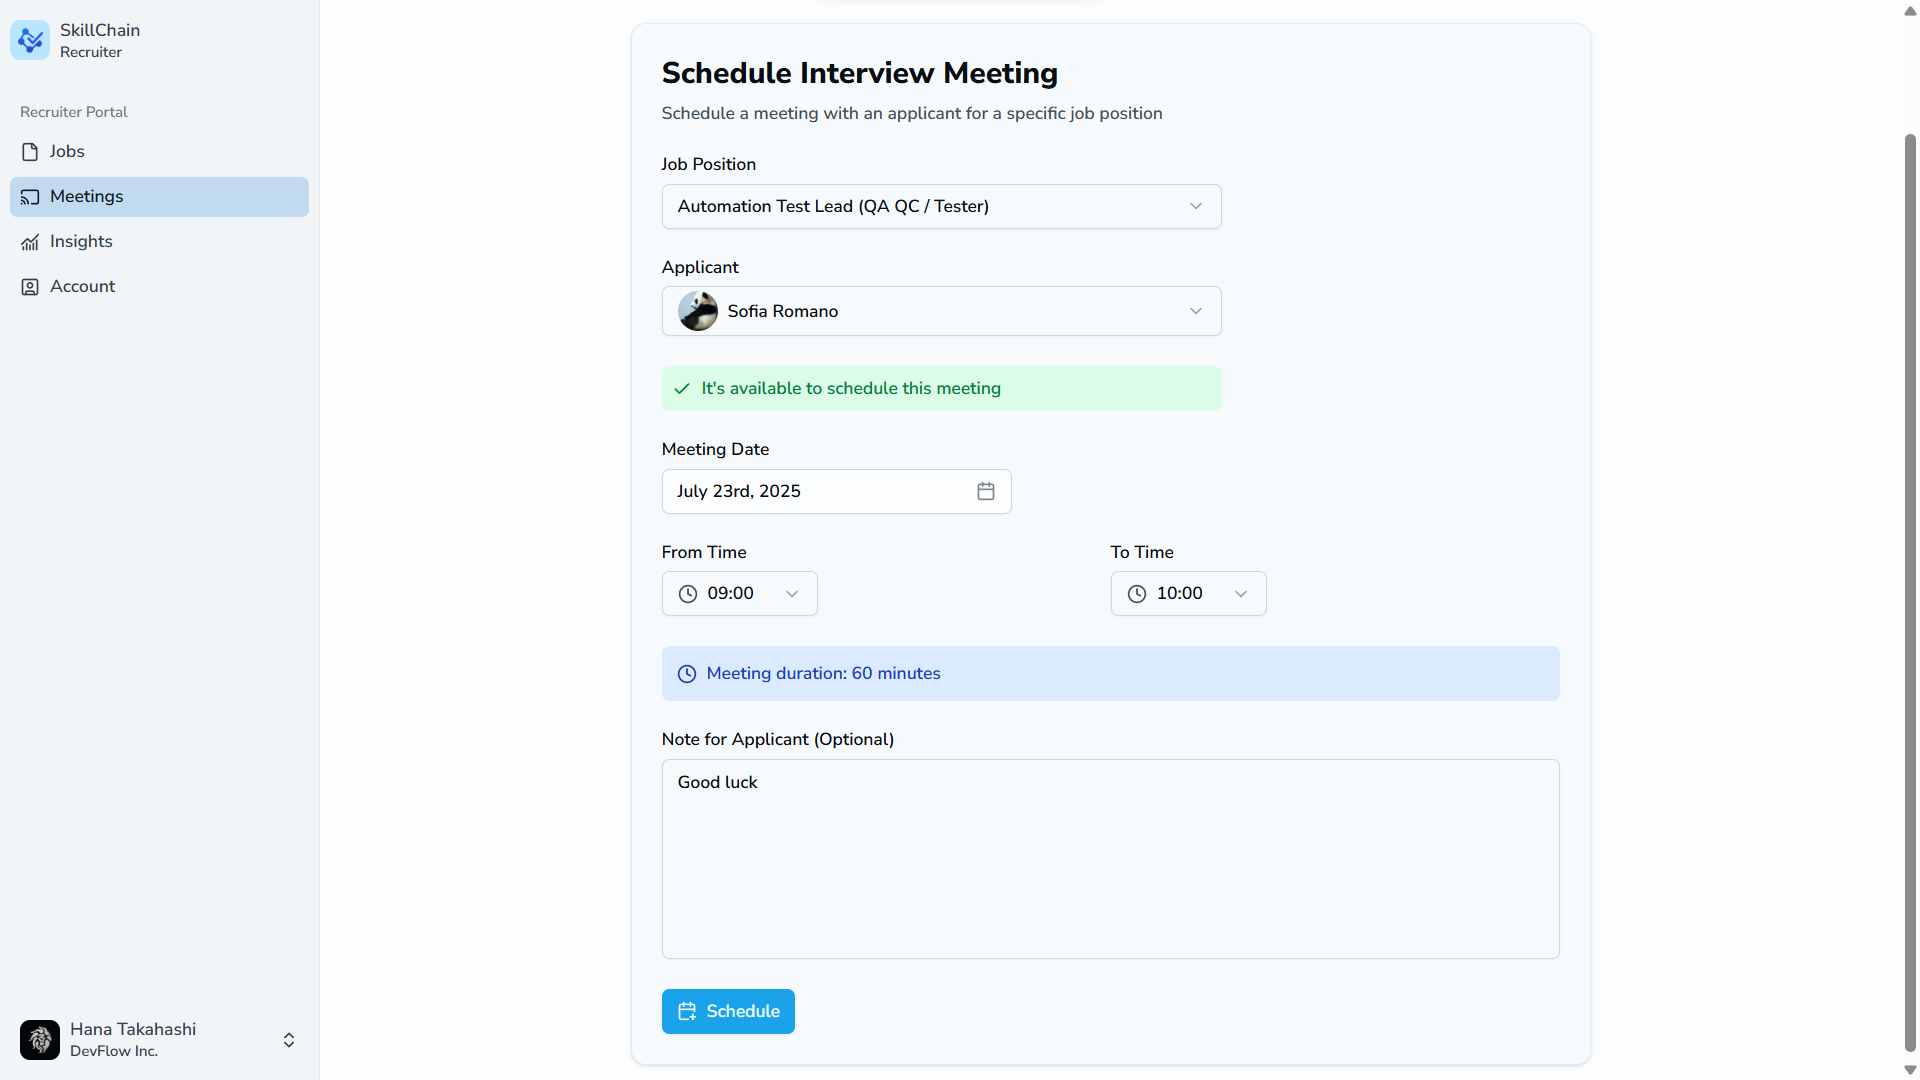
\includegraphics[width=0.99\textwidth, frame]{ui/schedule-meeting-form.png}
  \caption{Biểu mẫu lên lịch cuộc họp}
  \label{fig:schedule-meeting-form}
\end{figure}

\subsubsection{Đổi lịch một cuộc họp}

Đối với các cuộc họp ở trạng thái \textbf{đang chờ}, nhà tuyển dụng có thể thay đổi thời gian họp hoặc ghi chú bằng một trong hai cách:
\begin{itemize}
  \item Từ danh sách cuộc họp, chọn ``Reschedule'' tại mục ``Actions''.
  \item Từ trang chi tiết cuộc họp, nhấn ``Reschedule'' tại biểu tượng ba chấm ở góc trên bên phải.
\end{itemize}

\textbf{Lưu ý:} Không thể thay đổi vị trí công việc hoặc ứng viên đã được chọn.

\begin{figure}[H]
  \centering
  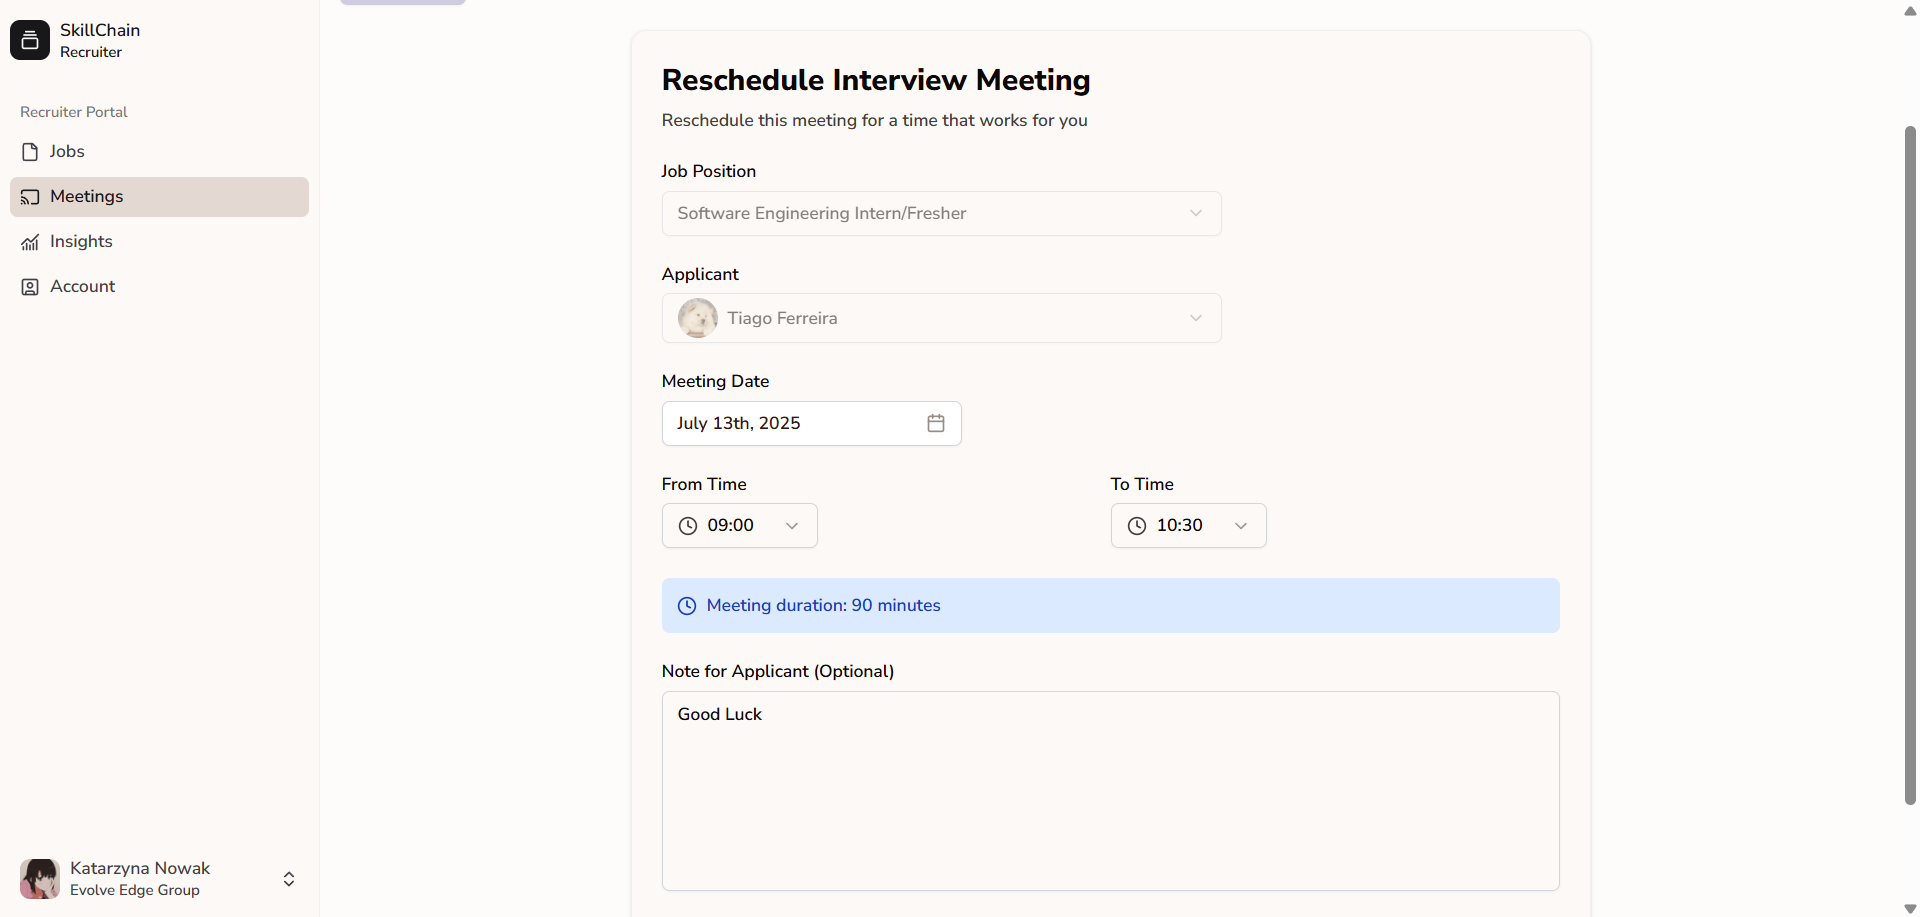
\includegraphics[width=0.99\textwidth, frame]{ui/reschedule-meeting-form.png}
  \caption{Biểu mẫu thay đổi lịch họp}
  \label{fig:reschedule-meeting-form}
\end{figure}

\subsubsection{Triển khai cuộc họp}

Khi đến thời điểm họp, tại trang chi tiết cuộc họp, nhà tuyển dụng nhấn nút ``Start Meeting'' để tạo và khởi chạy phòng họp trực tuyến.  
Hệ thống sẽ tạo liên kết tham gia và gửi đến ứng viên tương ứng.

\begin{figure}[H]
  \centering
  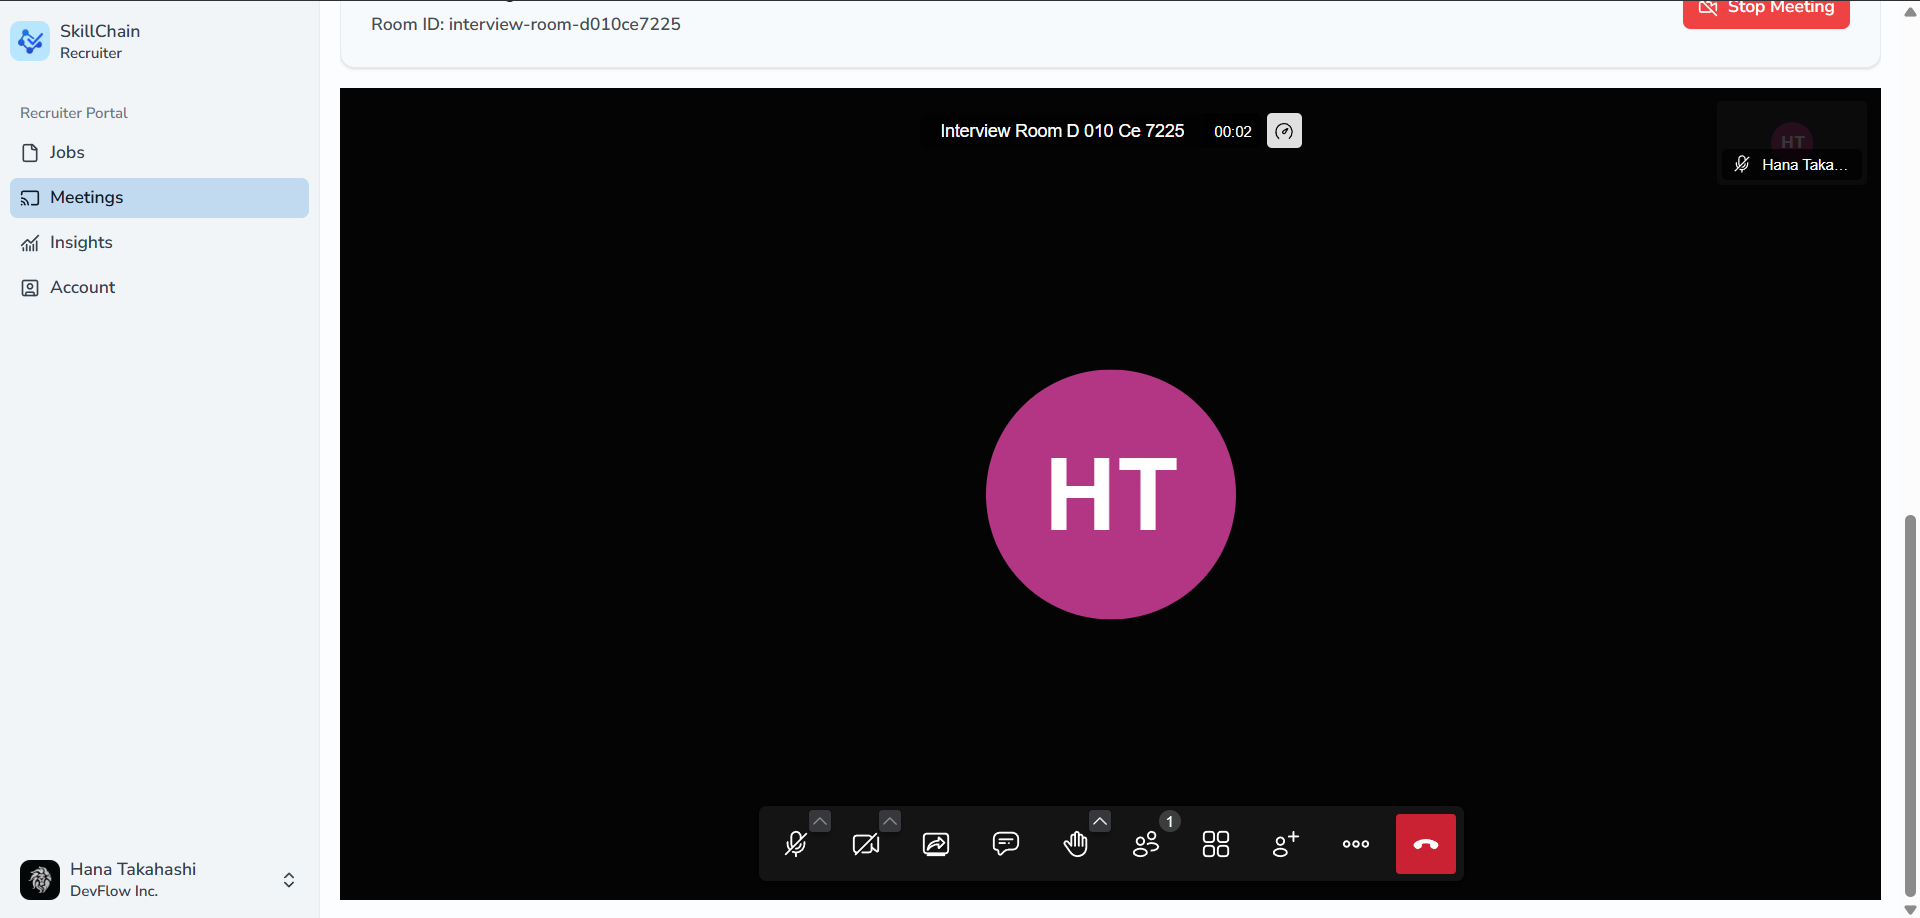
\includegraphics[width=0.99\textwidth, frame]{ui/meeting-hosting.png}
  \caption{Khởi chạy phòng họp trực tuyến}
  \label{fig:meeting-hosting}
\end{figure}

\subsection{Số liệu thống kê}

Để xem các số liệu thống kê liên quan đến quá trình tuyển dụng, nhà tuyển dụng truy cập tab \textbf{Insights}.  
Tại đây, hệ thống hiển thị các chỉ số tổng quan giúp đánh giá hiệu quả hoạt động tuyển dụng.
Bốn chỉ số mặc định được hiển thị gồm:
\begin{itemize}
  \item \textbf{Active Jobs}: Số lượng bài đăng tuyển dụng đang hoạt động.
  \item \textbf{Total Applicants}: Tổng số lượng ứng viên đã ứng tuyển.
  \item \textbf{Conversion Rate}: Tỷ lệ chuyển đổi từ ứng tuyển sang đã tuyển.
  \item \textbf{Pending Meetings}: Số lượng cuộc họp đang chờ diễn ra.
\end{itemize}

\begin{figure}[H]
  \centering
  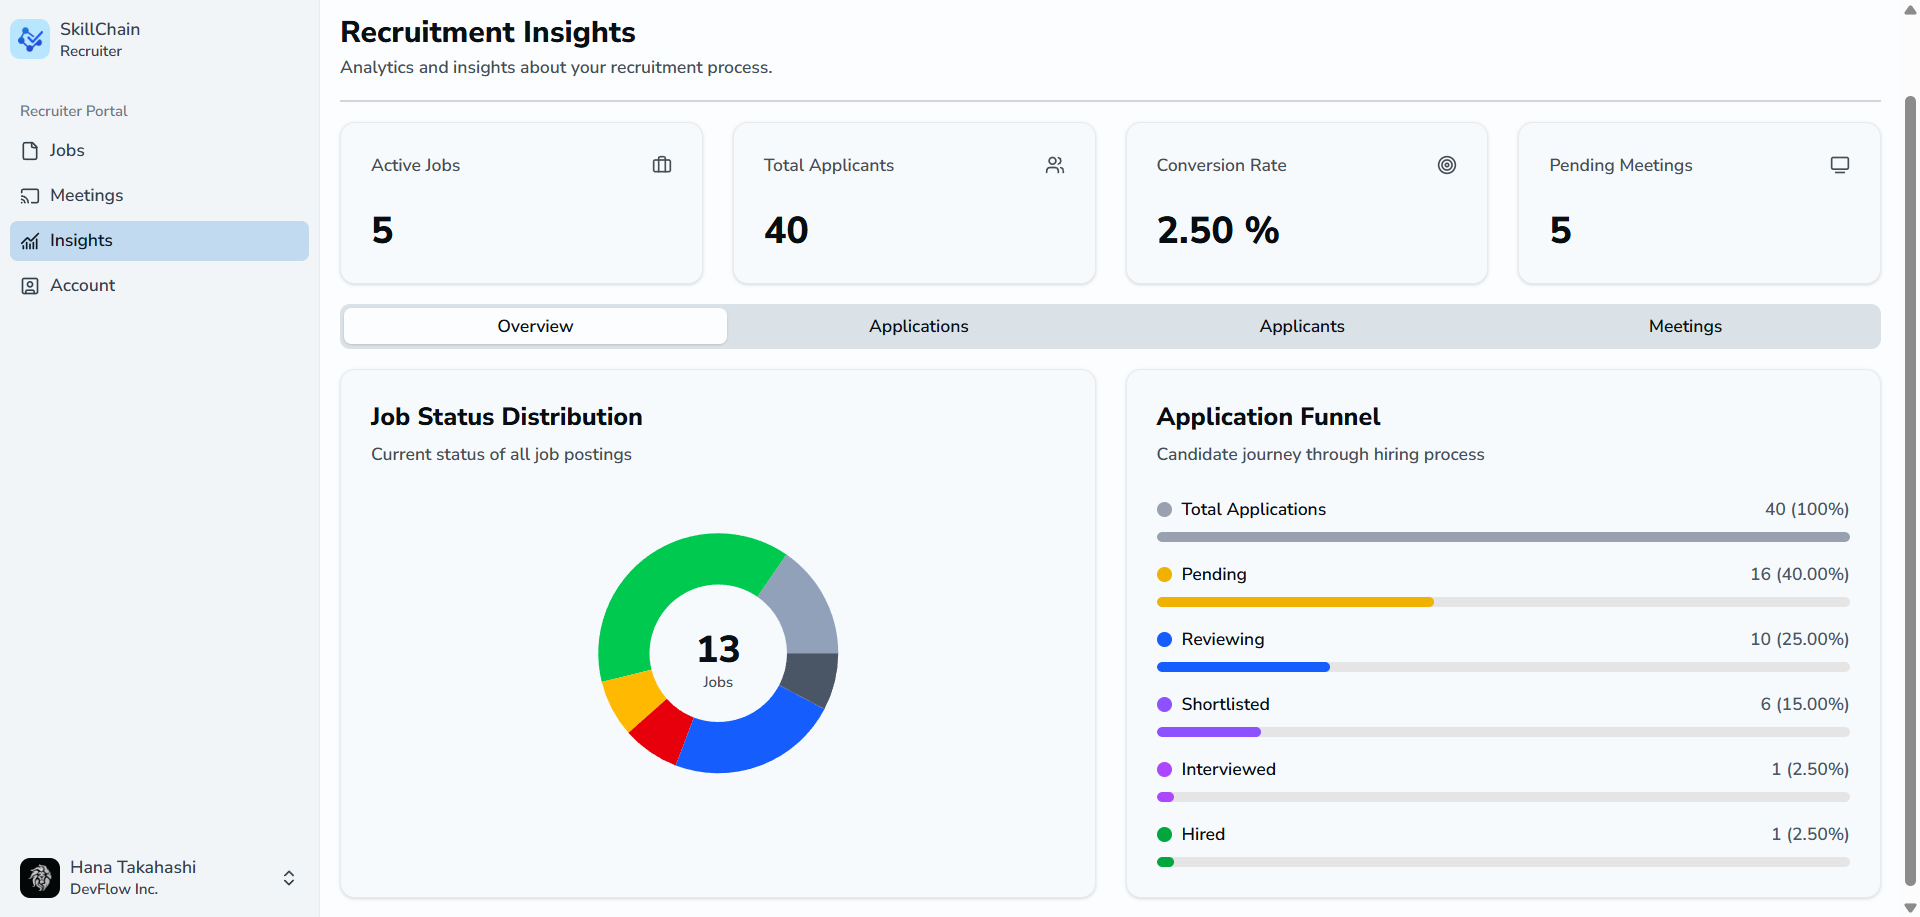
\includegraphics[width=0.99\textwidth, frame]{ui/recruiment-insight-page.png}
  \caption{Trang thống kê quá trình tuyển dụng}
  \label{fig:recruiment-insight-page}
\end{figure}

\subsubsection{Tab tổng quan (Overview)}

Tab \textbf{Overview} hiển thị hai biểu đồ trực quan:
\begin{itemize}
  \item \textbf{Job Status Distribution}: Biểu đồ tròn thể hiện số lượng các trạng thái bài đăng tuyển dụng (đang mở, đã đóng, nháp, v.v.).
  \item \textbf{Application Funnel}: Biểu đồ hình phễu mô tả tỷ lệ và số lượng ứng viên ở một số giai đoạn trong quy trình tuyển dụng.
\end{itemize}

\subsubsection{Tab ứng tuyển (Applications)}

Tab \textbf{Applications} hiển thị danh sách \textbf{Top 5 công việc có hiệu suất tốt nhất}, dựa trên:
\begin{itemize}
  \item Số lượng ứng viên ứng tuyển.
  \item Tỷ lệ chuyển đổi từ ứng viên sang đã tuyển dụng.
\end{itemize}

\begin{figure}[H]
  \centering
  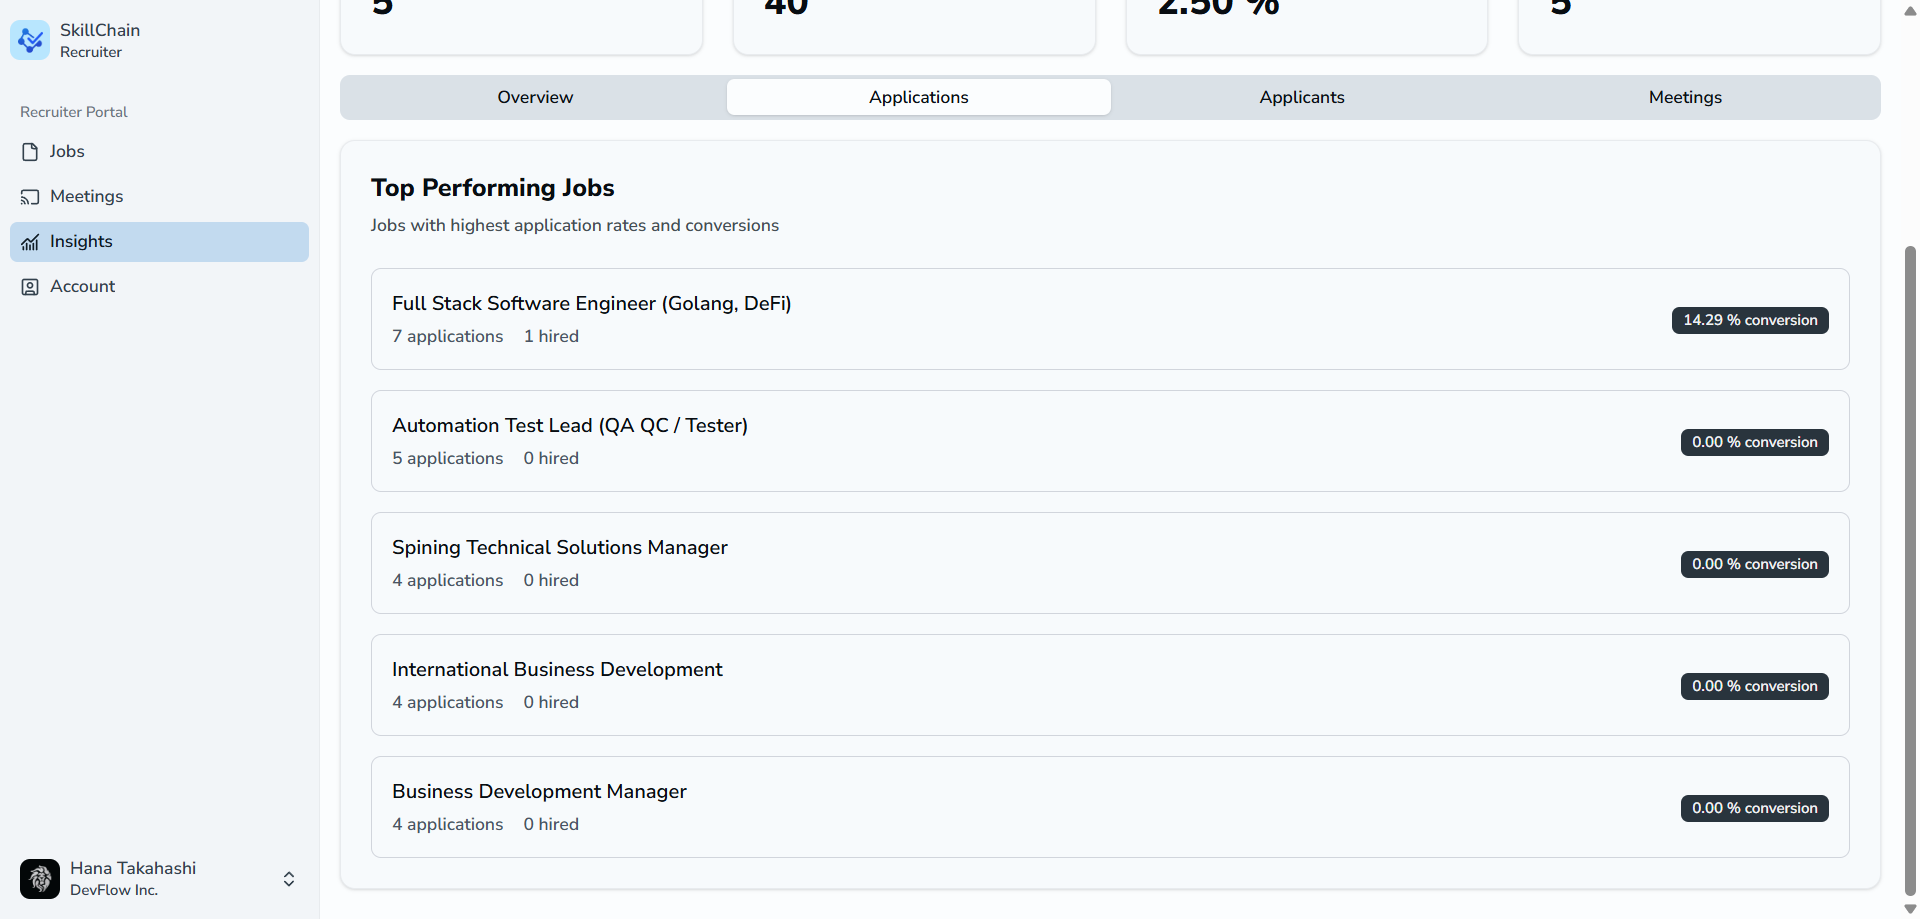
\includegraphics[width=0.99\textwidth, frame]{ui/top-performing-jobs.png}
  \caption{Năm công việc có hiệu suất tuyển dụng cao nhất}
  \label{fig:top-performing-jobs}
\end{figure}

\subsubsection{Tab ứng viên (Applicants)}

Tab \textbf{Applicants} hiển thị \textbf{Top 5 ứng viên tương tác nhiều nhất}, được đánh giá dựa trên số lượng bài đăng từ nhà tuyển dụng mà họ đã ứng tuyển.

\begin{figure}[H]
  \centering
  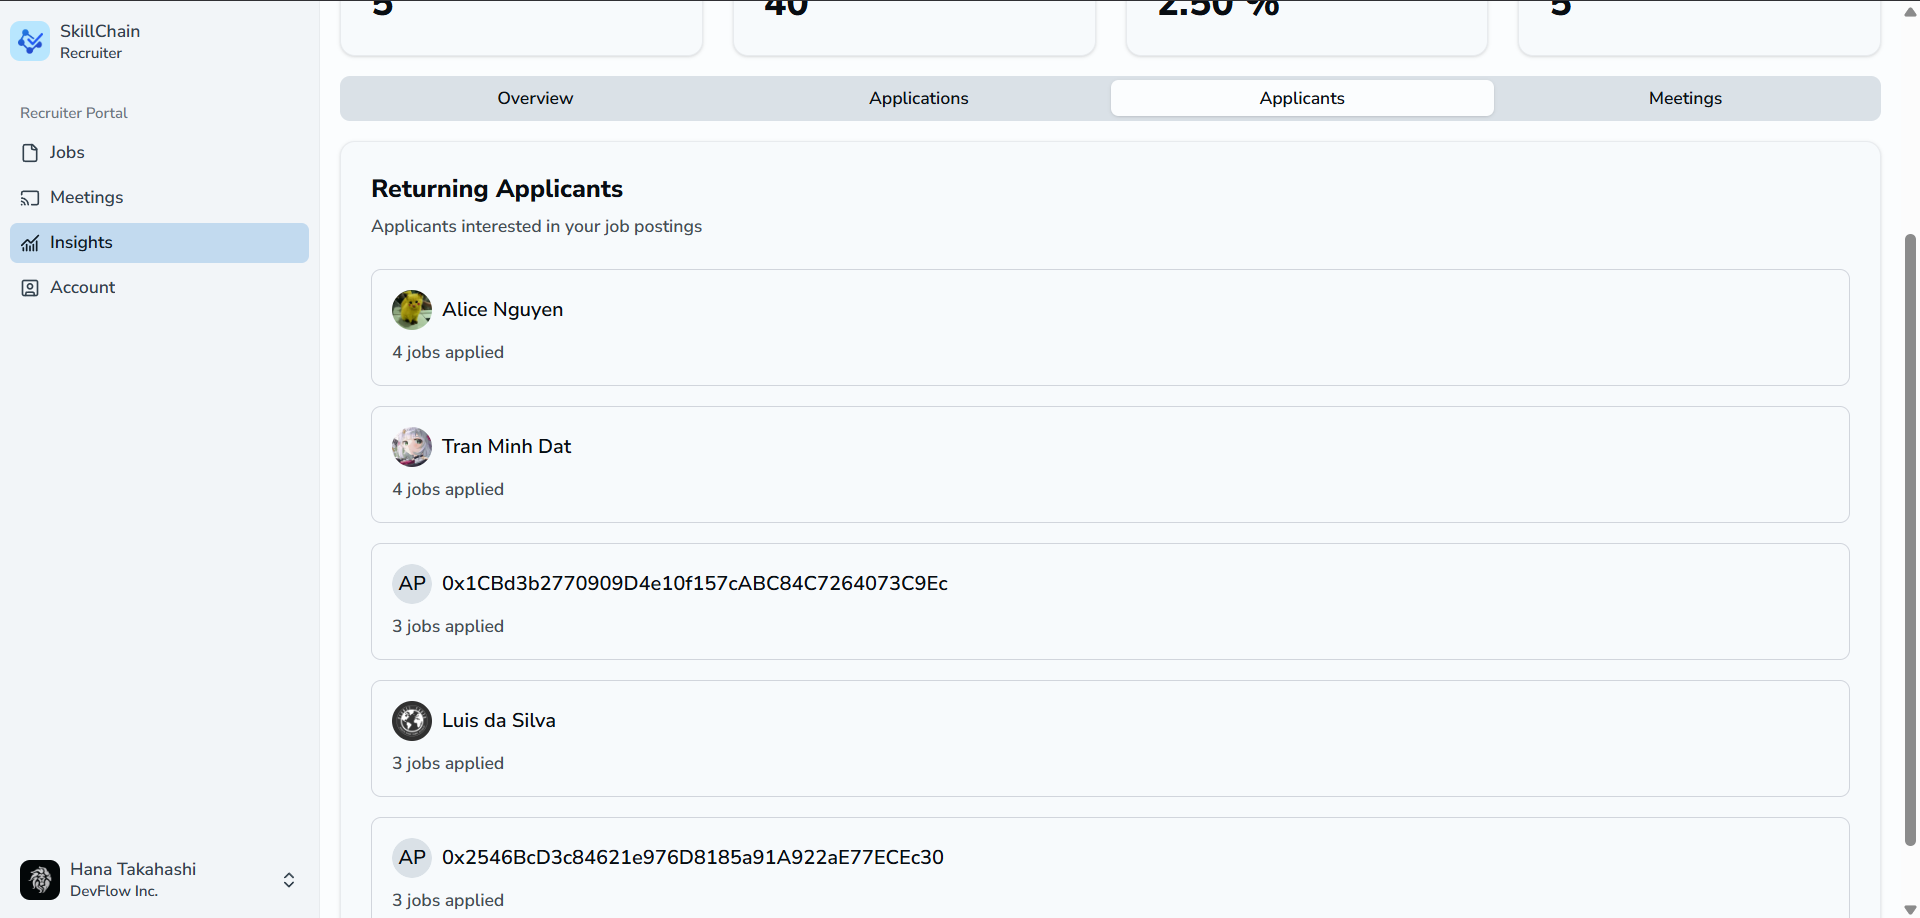
\includegraphics[width=0.99\textwidth, frame]{ui/top-returning-applicants.png}
  \caption{Năm ứng viên tương tác nhiều nhất với nhà tuyển dụng}
  \label{fig:top-returning-applicants}
\end{figure}

\subsubsection{Tab cuộc họp (Meetings)}

Tab \textbf{Meetings} cung cấp:
\begin{itemize}
  \item \textbf{Meeting Status Distribution}: Biểu đồ phân bố trạng thái các cuộc họp (đã hoàn thành, đang chờ, đã huỷ).
  \item \textbf{Upcoming Meetings}: Danh sách những cuộc họp sắp diễn ra, giúp nhà tuyển dụng chủ động chuẩn bị.
\end{itemize}

\begin{figure}[H]
  \centering
  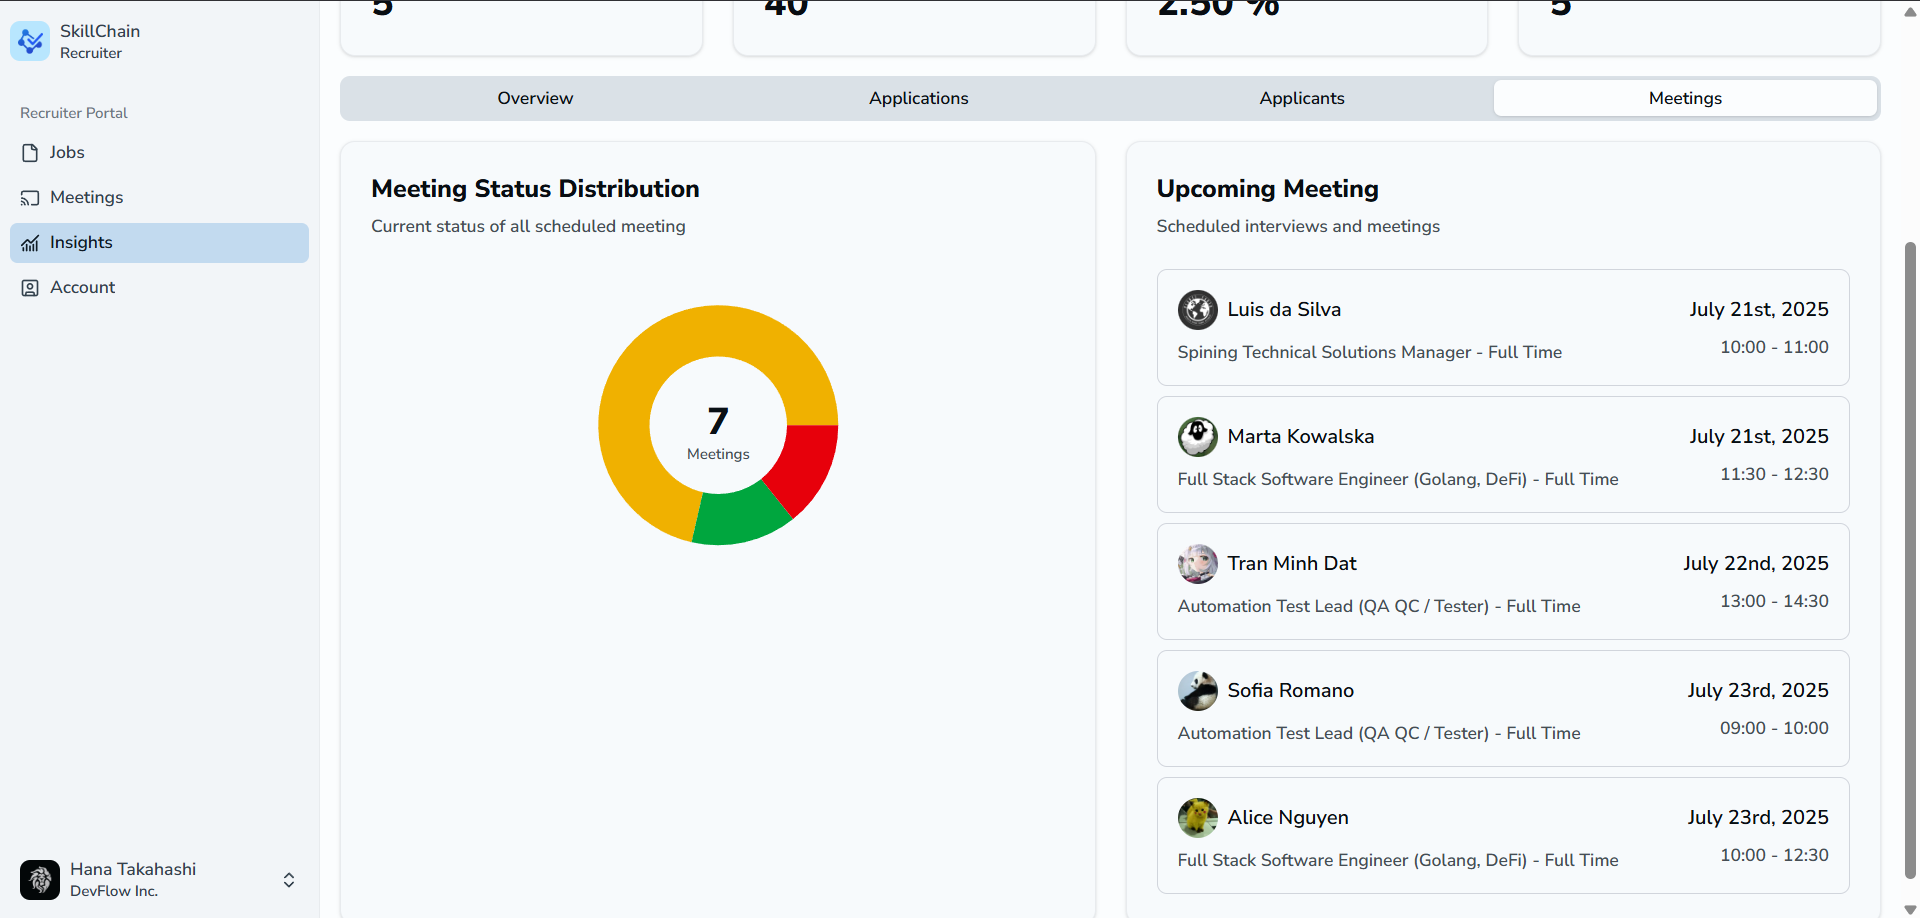
\includegraphics[width=0.99\textwidth, frame]{ui/insight-meetings-tab.png}
  \caption{Thống kê về các cuộc họp phỏng vấn}
  \label{fig:insight-meetings-tab}
\end{figure}

\subsection{Người dùng tham gia ứng tuyển}

\subsubsection{Xem danh sách công việc đang mở}

Để xem danh sách các công việc đang tuyển dụng, người dùng truy cập \textbf{Career} $\rightarrow$ \textbf{Available Jobs} trong không gian xây dựng uy tín.

\begin{figure}[H]
  \centering
  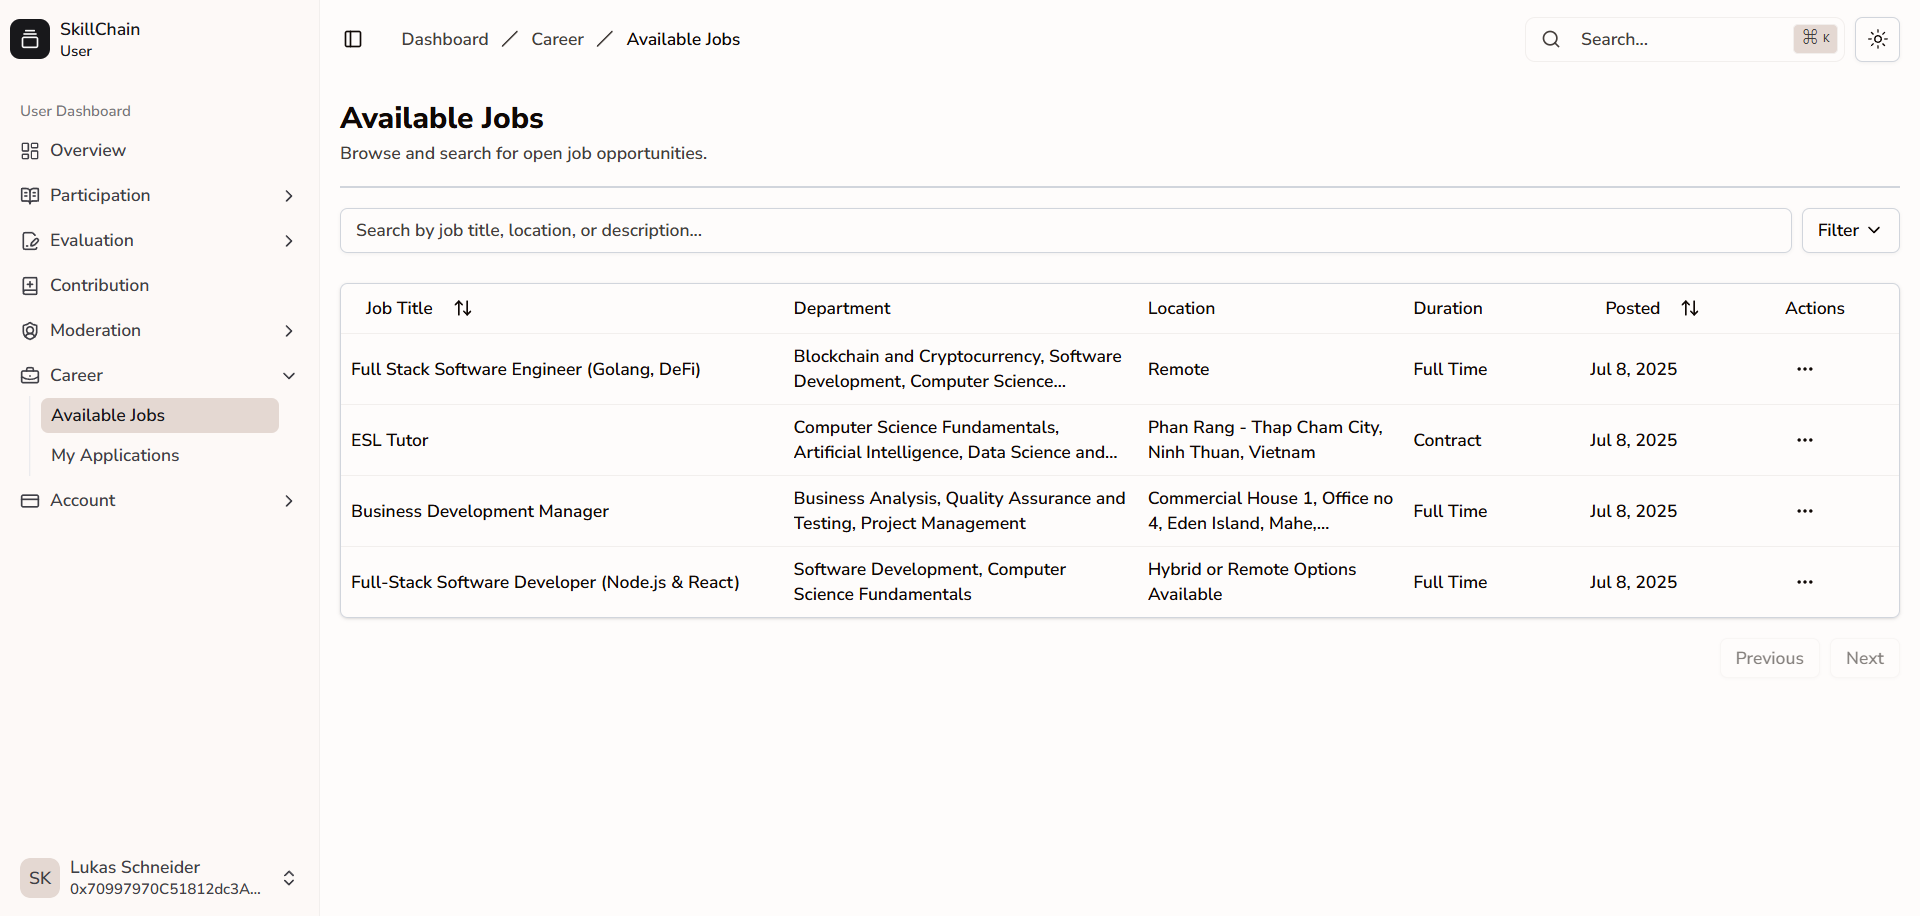
\includegraphics[width=0.99\textwidth, frame]{ui/available-jobs-page.png}
  \caption{Trang các công việc đang mở}
  \label{fig:available-jobs-page}
\end{figure}

Tại đây, người dùng có thể xem thông tin cơ bản của từng công việc như vị trí tuyển dụng, yêu cầu uy tín hay thời gian làm việc. 
Để xem chi tiết, nhấn nút ``View job'' tại mục ``Actions'' tương ứng.

\begin{figure}[H]
  \centering
  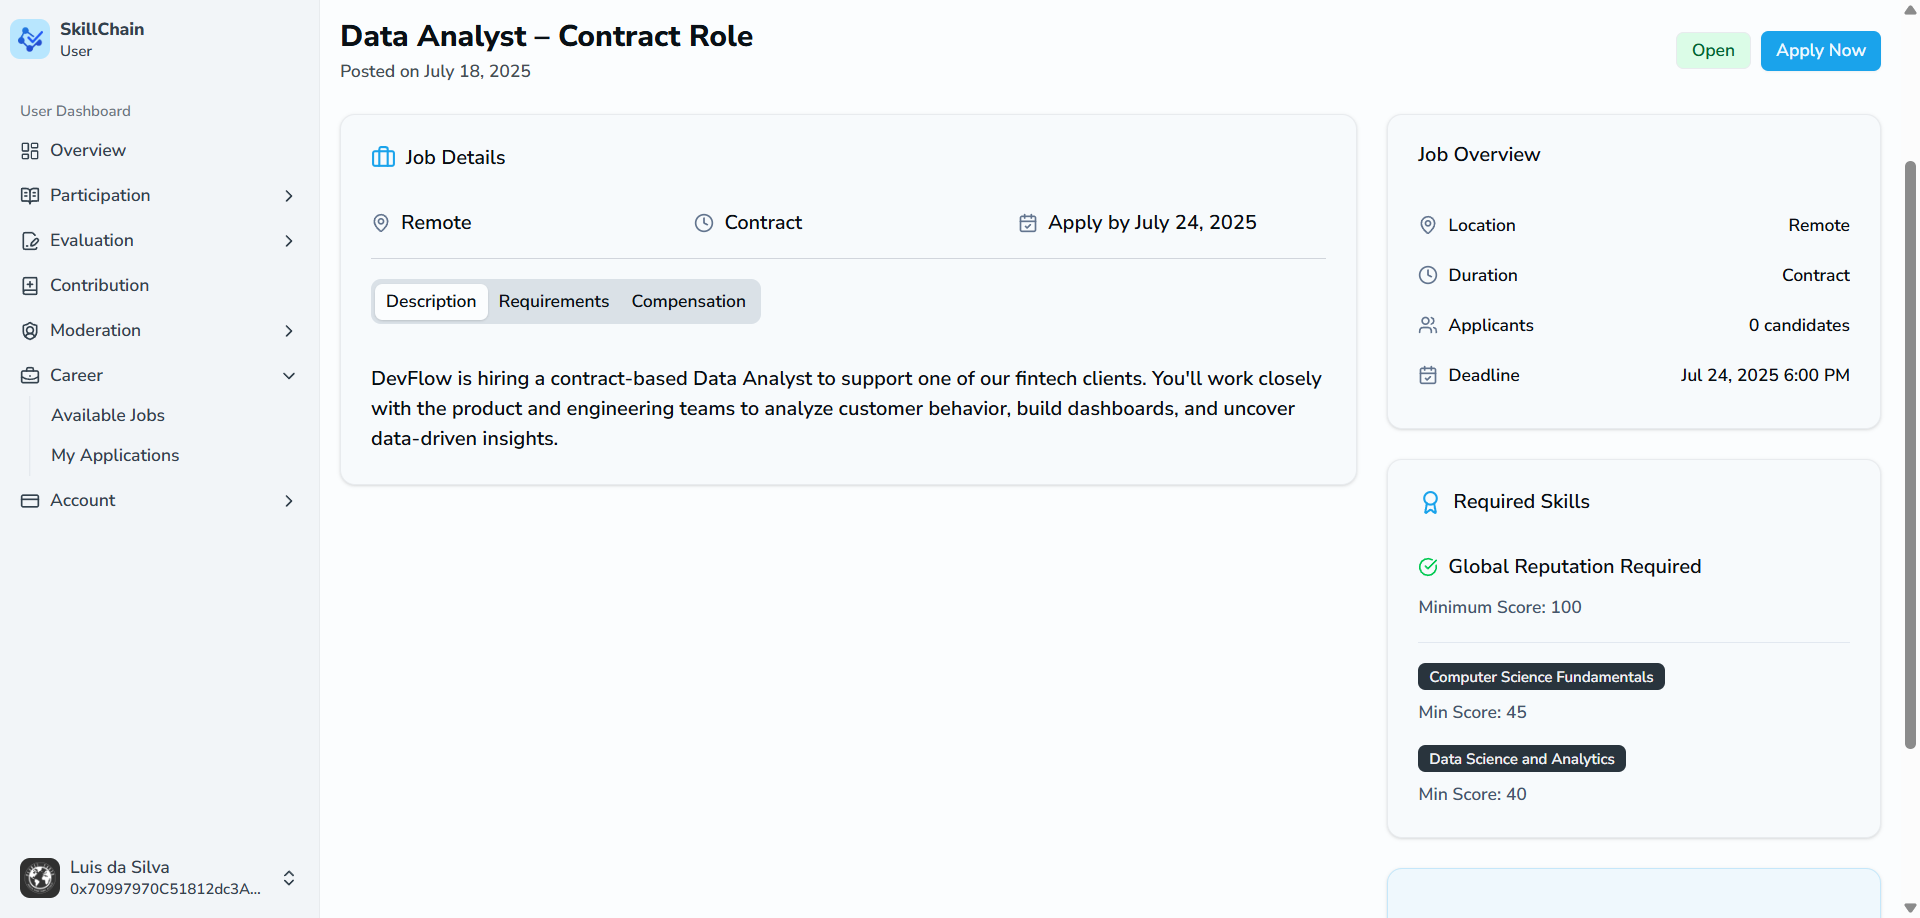
\includegraphics[width=0.99\textwidth, frame]{ui/available-job-detail-page.png}
  \caption{Trang chi tiết một công việc}
  \label{fig:available-job-detail-page}
\end{figure}

\subsubsection{Tham gia ứng tuyển}

Khi truy cập trang chi tiết công việc, hệ thống sẽ tự động kiểm tra mức độ uy tín của người dùng. Nếu không đáp ứng yêu cầu, hệ thống sẽ hiển thị thông báo và vô hiệu hóa nút ứng tuyển. 
Nếu đủ điều kiện, người dùng có thể nhấn nút ``Apply'' ở góc trên bên phải để nộp đơn ứng tuyển. Hành vi này yêu cầu xác nhận giao dịch thông qua ví tiền điện tử.

\subsubsection{Xem các công việc đã ứng tuyển}

Để theo dõi các công việc đã ứng tuyển, người dùng truy cập \textbf{Career} $\rightarrow$ \textbf{My Applications}. Tại đây, hệ thống hiển thị danh sách các công việc mà người dùng đã nộp đơn cùng với trạng thái tương ứng.

\begin{figure}[H]
  \centering
  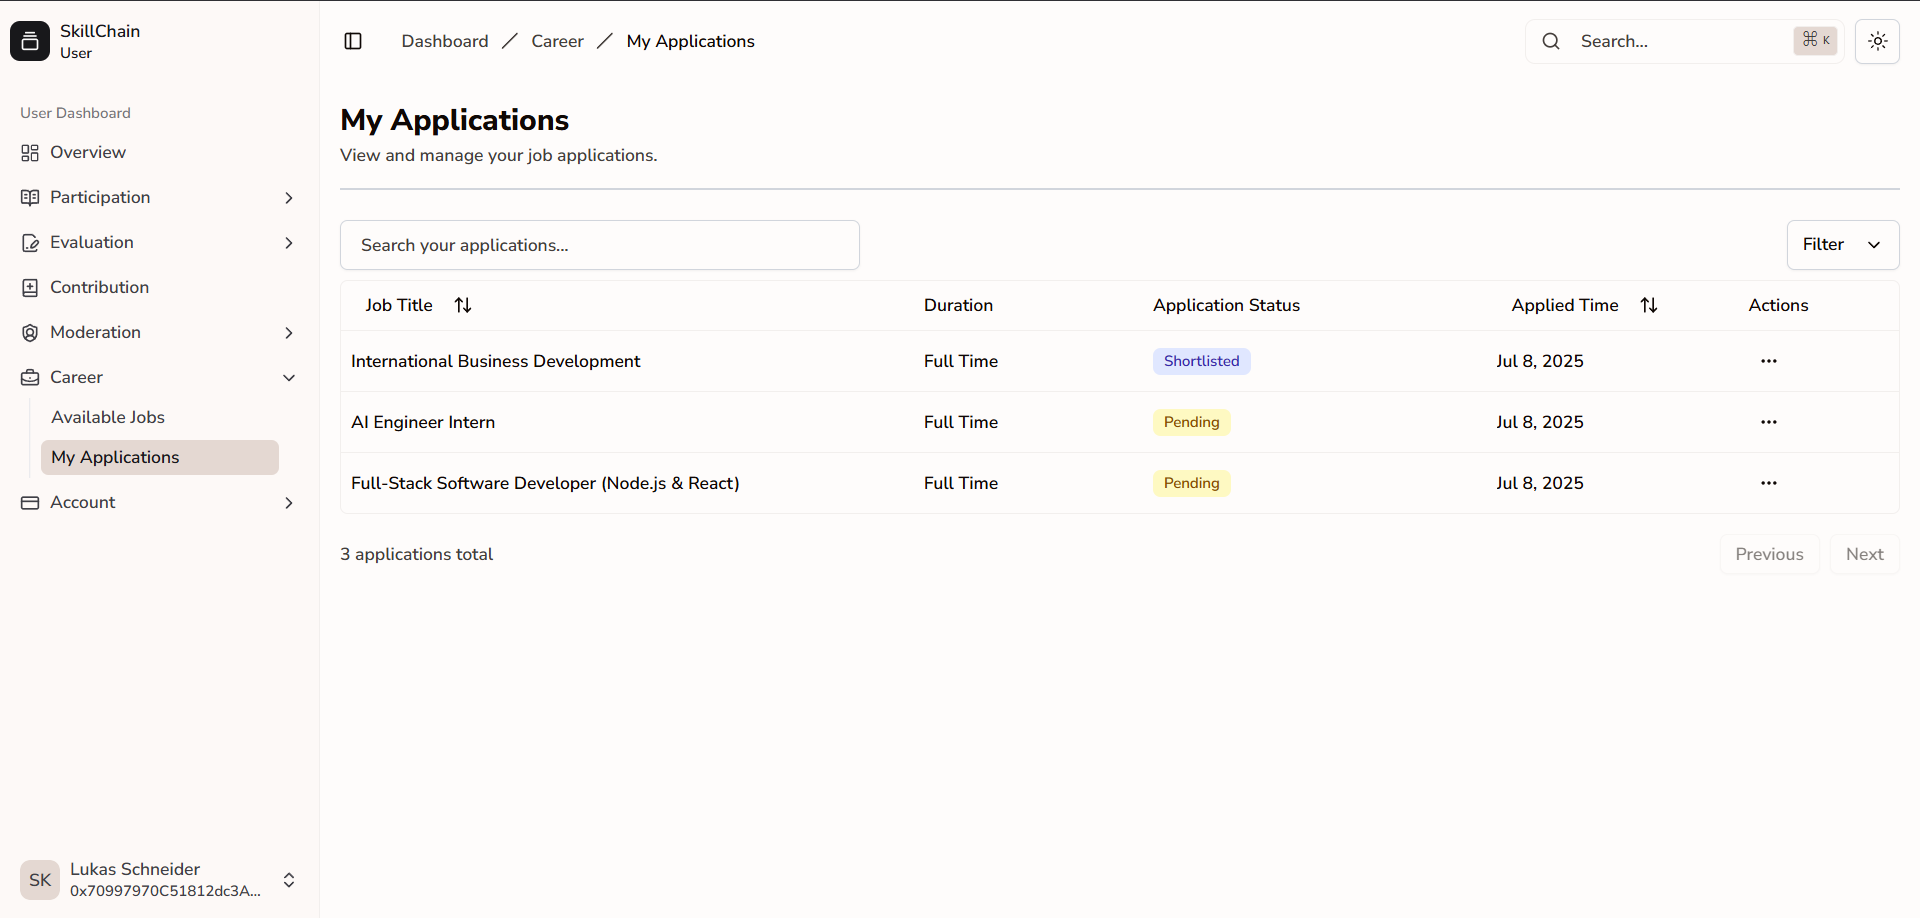
\includegraphics[width=0.99\textwidth, frame]{ui/my-applications-page.png}
  \caption{Trang công việc đã ứng tuyển}
  \label{fig:my-applications-page}
\end{figure}

Để xem thông tin chi tiết của một đơn ứng tuyển, nhấn ``View application'' tại nút ``Actions'' của công việc tương ứng. 
Trong trường hợp người dùng được đưa vào danh sách rút gọn, hệ thống sẽ hiển thị thêm thông tin lịch họp và liên kết tham gia phòng họp trực tuyến (nếu nhà tuyển dụng đã lên lịch).

\begin{figure}[H]
  \centering
  \includegraphics[width=0.99\textwidth, frame]{ui/my-application-detail-page.png}
  \caption{Trang chi tiết của một đơn ứng tuyển}
  \label{fig:my-application-detail-page}
\end{figure}

\subsubsection{Rút đơn ứng tuyển}

Nếu người dùng muốn hủy ứng tuyển, có thể nhấn nút ``Withdraw Application'' ở góc trên bên phải tại trang chi tiết ứng tuyển. Hành vi này yêu cầu xác nhận giao dịch thông qua ví tiền điện tử.
Người dùng sau đó sẽ không thể ứng tuyển lại cho vị trí này nữa.